\documentclass[a4paper,11pt]{report}
\usepackage[]{amsmath}
\usepackage[]{physics} % \bra, \ket etc
\usepackage{graphicx} %Pour les figures je crois
\usepackage{hyperref}
\usepackage[
    backend=biber, 
    natbib=true,
    style=numeric-comp,
    sorting=none, %Pour faire apparaitre les refs dans l'ordre
    hyperref=true
]{biblatex} %Imports biblatex package
\addbibresource{bib_thesis.bib} %Import the bibliography file

\usepackage{amssymb} %quelques symboles dont gtrsim /lesssim
\usepackage{subcaption} % package pour faire des subfigures
\usepackage{multirow} % package pour multirow/multicolumn
\usepackage{booktabs} % package pour top/mid/bottom rule
\usepackage{tcolorbox} % toujours plus de boites
\usepackage{xcolor} % Pour avoir des couleurs dans les équations

\DeclareUnicodeCharacter{0308}{HERE!HERE!} % je vais pas m'énerver, mais un peu quand meme

\title{}
\begin{document}
\begin{refsection}

\chapter{Introduction to Nitrogen-Vacancy centers and their common usage}
The aim of this first chapter is to introduce concepts related to Nitrogen-vacancy (NV) centers, to the diamond material, and to the dipole-dipole interaction which are necessary to explain the work presented in the later chapters.

In this introductory chapter, we will first cover the material aspects of NV centers by focusing on the creation process of synthetic diamonds and the required steps to create NV defects inside them. We will then cover the fundamentals of NV physics, including the NV center optical and spin properties, basic experiments with NV centers and the various relaxations times ($T_1$,$T_2$,$T_2^*$) which characterizes the NV center's spin. Finally we will present the dipole-dipole interaction between two spins and the concept of cross-relaxation.

\section{The NV center as a physical object}
\begin{figure}[h!]
\centering
\includegraphics[width=0.9\textwidth]{chapter 1/Figures/diamant_et_NV}
\caption{From the diamond to the NV center. a) Drawing of a bulk diamond. We consider a diamond to be ``bulk" if it is bigger than a few 100 $\mu$m. b) Drawing representing a fluorescence microscopy image of a diamond surface. The red fluorescent spots symbolize NV centers photoluminescence. c) Zoom-in on the crystalline structure of an NV center. Black balls represent carbon atoms}
\label{diamond+NV}
\end{figure}
The NV center is a particular defect in diamond. Before studying the NV centers properties, we must first discuss the diamond itself and answer these questions: How are diamond created, what kind of defects are there in diamond, and how to specifically create NV defects. The field of material science related to diamonds and NV centers is a rich and complex one, and this section will only introduce basic notions regarding these subjects.

Fig. \ref{diamond+NV} illustrates the various scales to consider in the study of NV centers. Starting with a bulk diamond, typically few mm wide, then zooming-in on the diamond surface with an optical microscope to find fluorescent spots corresponding to the photoluminescence of NV centers. Standard confocal microscopy is limited in its resolution to the $\sim \mu$m range, but if it was possible to zoom-in even further, we would see the atomic structure of a few \AA \ illustrated in the last panel. 
\subsection{Diamond material overview}
\begin{figure}[h!]
\centering
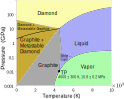
\includegraphics[width=0.6\textwidth]{chapter 1/Figures/phase_diagram_carbon_wiki}
\caption{Pressure-temperature phase diagram of elemental carbon. Credits: Wikimedia commons, adapted from \citep{bundy1989pressure, bundy1996pressure}.}
\label{carbon phase diagram}
\end{figure}

Diamond is a remarkable material in many aspects, it is famous for having the highest hardness and thermal conductivity of any natural material, and for its high optical refractive index and optical dispersion which makes it an extremely valuable crystal in jewelry.

Diamond is also famous for being extremely rare in nature, even though its only constituent, carbon, is one of the most abundant element on the Earth surface. The reason being that graphite, and not diamond, is the thermodynamically stable phase of carbon under ambient conditions.

Fig. \ref{carbon phase diagram} shows the PT phase diagram of elemental carbon. We can see that diamond becomes the thermodynamically stable phase only for pressure above a few GPa, $10^4$ times higher than atmospheric pressure. Even though diamond is unstable under ambient conditions, the extremely high energy activation needed to break the sp$^3$ bond between two carbon atoms means that the kinematics of the $C_{\rm diamond} \to C_{\rm graphite}$ transition is almost completely frozen. In many ways diamonds are more stable than graphite under ambient condition due to their relative chemical inertness.

Where the thermodynamic equilibrium really matters is for the crystallization process. The higher pressure needed to reach the diamond-stable region can only be found naturally deep under the earth crust, typically between 150 and 240 km below sea level \citep{tappert2011diamonds}, which explain their rarity. It also explains why, despite many previous attempts, diamonds were only synthetically produced in 1953 \citep{barnard2000diamond}, more than 50 years after the first synthetic sapphires. To this day, artificial diamond synthesis remains an active field of research \citep{shenderova2019synthesis, achard2020chemical}.

Diamonds, either natural or artificial, are used in the lab and in industry for their extreme sturdiness, with applications ranging from abrasive to diamond anvil cells \citep{jayaraman1983diamond}. More recently, diamonds have been the object of optics and electronics applications. For both of these fields however, the focus is no longer solely on the diamond but also on the defects hosted inside it.

\subsection{Point defects in diamond}
\begin{figure}[h!]
\centering
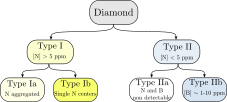
\includegraphics[width=0.9\textwidth]{chapter 1/Figures/Diamond_type}
\caption{Traditional classification of diamonds, based on \citep{tappert2011diamonds}}
\label{diamond type}
\end{figure}
Diamond in its intrinsic form is an insulator with a bandgap of $\sim 5.47\ \rm eV$ and is transparent from far infrared to deep UV. As any crystal however, diamond is prone to defects. We will focus here on point-like (0D) defects and omit structural defects such as dislocations, even though those too can affect the optical properties of the diamond \citep{collins2000colour}. 

Point-like defects can be constituted by the absence of a carbon atom (``vacancies"), an interstitial defect between two carbon atoms or the substitution of a carbon atom with another atom. These impurities result in unpaired electron or holes localized around the impurity site. This localization causes discrete energy levels for the holes or the electrons, some of which lie inside the diamond bandgap and impact the crystal optical and electrical properties. 

Defects with electronic transitions in the optical range are called ``colored centers" as they are responsible for the coloring of the gems.  Over 20 elements are known to form colored centers when introduced in diamond \citep{zaitsev2013optical, shenderova2019synthesis}, and each of these elemental atoms can form several defects. Nitrogen alone can form more than 50 different colored centers \citep{dobrinets2016hpht, ashfold2020nitrogen}.

Nitrogen, and to a lesser extant boron, are the most commonly found extrinsic elements in natural diamond. The traditional classification of diamond is presented in Fig. \ref{diamond type}. It is based on the N and B concentration, with a threshold of a few ppm (part per million) for each species as this was the smaller amount easily detectable through IR absorption. Type Ia diamonds contain clustered N defects such as the B-center (N$_4$V defect). In contrast, type Ib diamond mostly contains C-center which are single substitutional N$_s$ defects, also referred to as P1 centers in the spin community. Type IIb diamond contains boron impurities which give them a blueish-grey color, and type IIa diamond contains no detectable impurities via IR absorption \citep{ashfold2020nitrogen}.

Nitrogen-vacancy centers are a rare occurrence in both natural diamonds and untreated synthetic diamonds, but we will see later that the much more common N$_s$ defects can be converted in NV centers. When working with NV centers, the starting crystal is therefore often a type Ib diamond if one wants to work with ensemble, or a type IIa diamond if one wants to work with single NV centers \footnote{In order to isolate single NV in a confocal optical spot, the concentration needs to be [NV] $<$ 1 ppb.}.

The boron defects are mainly studied in the context of p-doped diamond semi-conductor: a concentration of [B] $\approx 1000\ \rm ppm$ is needed to achieve a significant overlap between the impurity sites, which turns the diamond into a semi-metal \citep{macpherson2015practical}. Other defects of interest, generally not present naturally but introduced voluntarily, include P and S defects to create n-doped diamond \citep{das2022diamond} (still an active field of research), as well as group IV-vacancy defects (SiV, GeV, SnV, PbV) for quantum optics application \citep{bradac2019quantum}. 

The NV center however remains by far the most studied defect in diamond due to its unique spin properties which will be detailed below.

\subsection{Creation of synthetic diamond for optics and electronics applications}
\begin{figure}[h!]
\centering
\includegraphics[width=\textwidth]{chapter 1/Figures/HPHT_and_CVD}
\caption{Schematics of HPHT (a) and CVD (b) growth process as detailed in main text}
\label{HPHT and CVD}
\end{figure}

Almost all diamonds used in optics or electronics experiments today are synthetic, due to the higher control of the growth process required for these applications. There are two main competing technologies for the growth of large ($\mu \rm{m} \sim \rm{mm}$) single crystal diamonds: High pressure high temperature growth (HPHT) and chemical vapor deposition growth (CVD). Both of these processes have their own specificities which are detailed below.

\subsubsection{HPHT growth}

HPHT was the first commercially viable process for synthetic diamonds, starting from the 1950s \citep{barnard2000diamond, bundy1955man}. The basic idea of HPHT synthesis is to reconstruct an environment where diamond is the thermodynamically stable phase of carbon, similarly to the growth process of natural diamond below the earth surface. 

Fig. \ref{HPHT and CVD}-a) illustrates the apparatus of HPHT synthesis: a carbon source (graphite) and a solvent metal composed of transition metals (Fe, NI, Co typically \citep{bundy1963direct}) are put under $5 \sim 6$ GPa pressure in a press and heated to temperatures $\geq 1300\ ^\circ$C. A diamond crystal seed is put in the metal melt and a temperature gradient insures that the carbon migrates from the graphite to the diamond.

The first synthesis of HPHT diamonds were all of type Ib due to unwanted nitrogen pollution in the metal melt. The first HPHT type IIa diamonds were produced in the late 90s by adding other elements to the metal bath (Ti, Al, Zr) which would react preferentially with nitrogen and prevent its incorporation in the diamond \citep{burns1999growth, sumiya2002growth}.

\subsubsection{CVD growth}

Diamond growth by CVD also started in the 50s, but the first reasonable growth rates were only achieved in the 80s \citep{matsumoto1982growth, matsumoto1982vapor, kamo1983diamond}. Unlike HPHT, CVD operates in a regime where diamond is not the thermodynamically stable phase. It relies therefore heavily on catalysts to stabilize the diamond phase versus the graphite one. 

The main catalyst used is atomic hydrogen because it etches the $C-C$ sp$^2$ bonds (graphite) faster than it does sp$^3$ bonds (diamond) \citep{gracio2010diamond}. In modern CVD growth, hydrogen is by far the most abundant element in the gas phase: the precursor gases used for the growth are typically CH$_4$ and H$_2$ in proportions of $1-5\%$ and $95-99\%$ respectively \citep{achard2020chemical}.

Fig. \ref{HPHT and CVD}-b) illustrates the apparatus of a microwave plasma reactor: it consists in a modified vacuum chamber which acts as a microwave resonator. The microwave creates a plasma ball from the the precursor gases with a temperature $T_{\rm plasma} \geq 3000 ^\circ$C \citep{ashfold2020nitrogen}, enough to dissociate the $H_2$ gas in atomic hydrogen \citep{balmer2009chemical}. The plasma acts as the carbon source for the diamond growing on top of the substrate, and as the catalyst to favor the diamond phase. The substrate is kept at a temperature $700 \sim 1100\ ^\circ$C during the growth.

Other sources can be used to create the high temperature required for atomic hydrogen, such as a tungsten hot filament \citep{haubner1993diamond}, electrical discharge (arcjet) \citep{luque1998excited} or even an oxygen-acetylene combustion flame \citep{bachmann1991towards}.

If the CVD reactor is well made, the main sources of extrinsic impurities in the diamond comes from the source gasses \citep{balmer2009chemical}. The commercial availability of source gases containing less than $\sim$ ppm impurities made possible the growth of  high purity type IIa CVD diamonds \citep{kasu2003high, twitchen2004high, tallaire2006characterisation}.

\medskip
Both HPHT and CVD processes can produce diamonds of high quality for quantum optics or electronics application, each with their own pros and cons. HPHT offers better scalability for thick crystals ($\sim \rm mm$) and allows the incorporation of heavy atoms (Ge \citep{palyanov2015germanium} , Sn \citep{ekimov2019effect}) which can be hard to incorporate from a gas phase. CVD on the other hand allows more versatility in the control of the impurities introduced in the crystal, including an isotopic control on both the impurities and the carbon itself. A particular advantage of CVD growth is the possibility of $\delta$-doping where a specific defect is grown only within a thin layer of the crystal, as low as 5 nm \citep{ohno2012engineering, ishikawa2012optical, ohashi2013negatively}.

\subsection{Optimizing NV center formation}
\begin{figure}[h!]
\centering
\includegraphics[width=\textwidth]{chapter 1/Figures/formtion_NV_2}
\caption{Illustration of the formation of NV centers. Black dots represents carbon atoms and green dots nitrogen atoms}
\label{formation NV}
\end{figure}

NV centers are a relatively rare impurity in untreated diamonds. In CVD diamond for instance, the proportion of nitrogen atoms forming an NV center in an untreated crystal is at best of $2-3 \%$ \citep{hartland2014study} and oftentimes much lower. While this ratio can be enough  to work with single NV centers, applications such as sensing that require dense ensemble need a higher conversion rate. We will discuss here the usual techniques employed to improve the formation of NV centers.

Fig. \ref{formation NV} illustrates the steps needed to maximize the number of NV centers in the crystal while keeping a relatively high crystalline purity.

The first step to create NV centers is to get individual substitutional N atoms in the crystal ($N_s$, C-centers or P1 centers depending on the literature). This can be achieved either \textit{in situ} by introducing (voluntarily or not) nitrogen in the crystal during the growth process \citep{tallaire2006characterisation, lobaev2017influence}, or \textit{ex situ} by implanting N$^+$ ions with ion implantation techniques \citep{meijer2005generation, smith2019colour}. Because this present work focuses on dense NV ensembles, we will consider the simplest case where the starting crystal is a type-Ib diamond due to the presence of nitrogen during the growth. A starting concentration [N$_s$]= $10 \sim 300$ ppm is typical for type Ib HPHT diamonds \citep{achard2020chemical}.

The second step is to create monovacancies in the crystal lattice. This step might be optional for crystals which already contain a large number of monovacancies, but CVD crystals in particular can have less vacancies that they have substitutional nitrogen atoms \citep{mainwood1999point}. The general technique to create monovacancy is to bombard the sample with high energy particle in order to knock out carbon atoms from the crystal. Several high energy particle have been used to create vacancies, such as protons, electrons, ions, neutrons and even gamma rays \citep{davies1976optical, ashbaugh1988gemstone, kleinsasser2016high}. The most common irradiation source for for bulk diamond however is electron irradiation (e-beam) \citep{acosta2009diamonds}, thanks to their relatively frequent availability (compared to neutrons or gamma rays) and their ability to deeply penetrate the crystal.

The final step is to migrate the vacancies next to the nitrogen atoms. The activation energy required to move vacancy is of $\sim 2.3\ \rm eV$ which corresponds to temperatures of $600\sim 700 ^\circ$C \citep{davies1992vacancy, newton2002recombination}. The most common method to move the vacancies is therefore to anneal the crystal at a temperature $800 \sim 1200 ^\circ$C for a few hours \citep{botsoa2011optimal}. When the vacancy is next to a nitrogen atom, it will only become mobile again for temperatures of $1400 \sim 1500 ^\circ$C \citep{zaitsev2013optical, pinto2012diffusion} which explains why the annealing process favors NV creation.

The final N$_s$ to NV conversion rate can be as high as $\sim 50 \%$ \citep{grezes2015storage, hartland2014study}, although this ratio tend to decrease for higher [N$_s$] concentrations. Most sample studied in this manuscript had a concentration $[\rm NV]= 1-10\ \rm ppm$ (see [REF] samples)

\subsection{Controlling the NV center charge state}

The charge state of the NV center is of crucial importance for NV applications. Only the negatively charged NV$^-$ center shows the specific spin properties that will be detailed below, but the NV center can exist under three charge states in the diamond: NV$^-$, NV$^0$ and NV$^+$. The presence of NV$^+$ is usually marginal \citep{hauf2014addressing, pfender2017protecting} and we will focus here solely on the NV$^-$ and NV$^0$ charge state.

The charge state of the NV centers depends not only on the growth process of the crystal, but also on the experiment performed with the sample. In particular, illumination in the optical range can promote electrons in the conduction band or holes in the valence band and modify the charge state of the NV center.

On the material side, the crystal has to remain electrically neutral which means that at least as many charge donors need to be present as there are NV$^-$ centers. For nitrogen-rich samples, the donors are mostly N$^+$ centers, which imposes a limit on the maximum conversion rate of N to NV in order to keep a high [NV$^-$]/[NV$^0$] ratio. The possibility to introduce other donors, such as phosphorus, has been studied \citep{doi2016pure} but remains impractical so far \citep{barry2020sensitivity}.

On the experimental side, it has been shown that the ionization of NV$^-$ to NV$^0$ and the reverse process depend on the intensity and wavelength of the laser used for illumination \citep{aslam2013photo}. It was found that the optimal wavelength to preserve the NV$^-$ charge state was  $510-540\ \rm nm$. The most common wavelength used with NV centers is 532 nm (green) due to the historical importance of Nd:YAG lasers. On the other hand, it is possible to semi-permanently ionize the NV$^-$ into NV$^0$ when using a red excitation, which has been used to create optical memories \citep{dhomkar2016long}.

For samples in high excess of [N$_s$] such as type Ib HPHT diamonds, the question of the charge state of the NV center is of relatively low importance as the NV$^-$ state is the predominant one. For sample with a lower [N$_s$] content and a higher [NV]/[N$_s$] ratio however, one must be more careful with the optical intensity and wavelength used as the concentration of NV$^0$ can reach up to 50\% of the total NV concentration \citep{grezes2015storage}

\section{The NV$^-$ center optical and spin properties}

This section focuses on the NV$^-$ center properties both as an optical defect (colored center) and as a spin defect, and compare them to other solid state systems. It also covers the interplay between the spin and the optical levels, a property almost unique to the NV$^-$ center which is the basis for optical polarization and readout of the NV$^-$ spin state.

\subsection{NV center molecular orbitals}

\begin{figure}[h!]
\centering
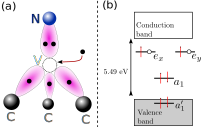
\includegraphics[width=0.8\textwidth]{chapter 1/Figures/NV_electrons}
\caption{(a) Representation of the nitrogen and carbon orbitals surrounding the vacancy of an NV center. Each black dot represents an electron. A sixth electron is required to form the negatively charged NV$^-$ state. (b) Molecular orbitals of the NV center predicted from the the $C_{3v}$ symmetry of the defect. The electron occupation of the NV$^-$ ground state is represented by red arrows.}
\label{NV electrons}
\end{figure}

We will first cover the molecular aspect of the NV defect in diamond and the energy levels of the defect predicted from group theory and ab initio computations.

Fig. \ref{NV electrons}-a) illustrates the $sp^3$ orbitals of the carbons and nitrogen atoms neighboring the vacancy, as well as the 5 electrons occupying dangling bonds from these atoms and a sixth electron captured to form the negatively charged NV$^-$ state. 

Fig. \ref{NV electrons}-b) shows the predicted molecular orbitals of the NV centers, initially computed as linear combination of the $sp^3$ orbitals respecting the $C_{3v}$ symmetry of the defect \citep{loubser1978electron}. This model has since been confirmed by ab initio computation and experimental observations \citep{doherty2013nitrogen}. In particular ab initio computations have shown that the molecular orbitals of the NV center are mostly localized on the nearest neighbors of the vacancy \citep{gali2008ab}. Ab initio computation has also determined that the $a'_1$ level lies in the valence band and is thus often ignored.

The electron occupations shown in Fig. \ref{NV electrons}-b) corresponds to the electronic ground state of the NV$^-$ charge state.

In the remaining part of this manuscript, we will only consider the negatively charged NV$^-$ state, unless specified otherwise. We will therefore omit the ``$-$" and simply refer to the negatively charged state as ``NV".
\subsection{Optical properties of the NV center}
\begin{figure}[h!]
\centering
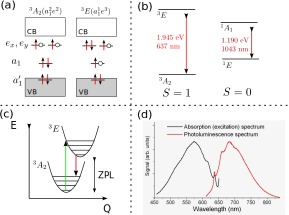
\includegraphics[width=1\textwidth]{chapter 1/Figures/NV_optical}
\caption{Optical properties of the NV center. (a) Electron occupation of the molecular orbitals for the electronic ground state $^3A_2$ and the first excited state $^3E$. (b) Diagram of the main optical transition between the two spin triplet states and of the IR transition between the two singlet sates. The value of the transition corresponds to the zero phonon line (ZPL) and are taken from \citep{doherty2013nitrogen}. (c) Representation of the vibronic structure for the $^3A_2$ and $3^E$ states under the Franck-Condon approximation. The graph axes are the energy of the states E and configuration coordinate q. The green and red arrow represents non-resonant (Stokes) absorption and emission. (d) Emission and absorption spectrum of the NV center main transition at 300 K, from PL and PLE measurements respectively. Credits: Wikimedia commons}
\label{NV optical}
\end{figure}

Because the NV center has discrete electronic transitions inside the diamond band gap, it fluoresces: it can absorb light from $450-650$ nm and re-emits light in the $600-800$ nm band.

Fig. \ref{NV optical} explains the origin of the NV center optical properties. Fig. \ref{NV optical}-a) illustrates the electronic ground state $^3A_2$ and first excited state $^3E$, where 1 electron from the $a_1$ molecular orbital is promoted to the $e$ level. Both of these electron occupations have two unpaired electrons, meaning that they can exist either either in a spin triplet state ($S=1$) or a spin singlet state ($S=0$) \footnote{The two singlet states $^1E$ and $^1A_1$ represented in Fig. \ref{NV optical}-b) are both of configuration $a_1^2e^2$ where the two $e$ electrons are either in a the same $e$ orbital, or in an antisymmetric superposition of the two $e$ orbitals \citep{doherty2011negatively}.}. 

Fig. \ref{NV optical}-b) shows the zero phonon line (ZPL) for the main transition of the triplet ($^3A_2$ and $^3E$) and singlet ($^1E$ and $^1A_1$) states. It should be noted that due to an inter system crossing between the $^1E$ and $^3A_2$ levels, excitation or absorption of the singlet transition is only possible with a conjoint excitation of the triplet states. By default, we refer to the NV center photoluminescence (PL) as the emission between the two triplet states.

Fig. \ref{NV optical}-c) illustrates the vibronic structure of the $^3A_2$ and $^3E$ states under the Franck-Condon approximation \citep{gali2011time}. The emission and absorption of light associated with the triplet transition can be accompanied by the emission or absorption of an optical phonon. Because the lifetime of the optical phonons is very short, the absorption or emission of light almost always start from the fundamental state of the $^3A_2$ and $^3E$ level, which explains why the absorption of light can only be done for energies above the ZPL, and the emission for energies below the ZPL (Stokes process).

Finally Fig. \ref{NV optical}-d) shows the absorption and emission spectrum of NV centers at 300 K. A weak zero-phonon-line is visible at 637 nm, with large phonon sidebands in emission and absorption.

\medskip
Compared to similar solid state photon sources (other color centers, quantum dots, dye molecules...), the NV center offer several advantages. First, they are very bright thanks to the $\sim 11\ \rm ns$ lifetime of the excited state and quantum efficiency of $0.7-0.8$ \citep{schirhagl2014nitrogen}. With proper nanophotonics engineering (solid immersion lenses or diamond waveguide) the PL collected from a single NV center can reach a few $10^6$ photons/s \citep{schroder2016quantum}.  Secondly, the NV center is also extremely photostable under green excitation, and does not show any photobleaching \citep{brouri2000photon}. Finally, the diamond itself is resistant to heat and chemical attacks, and presents low toxicity for biologic systems \citep{fu2007characterization}. There are however drawbacks in using NV centers for photonics applications, the main one being that $\leq 4\%$ of the photons emitted by the NV centers are in the ZPL (low Debye Waller factor), even at cryogenic temperature \citep{johnson2015tunable}. This limits the potential of NV centers for quantum photonic devices \citep{bradac2019quantum}.

\subsection{Spin properties of the NV center electronic ground state}
\begin{figure}[h!]
\centering
\includegraphics[width=1\textwidth]{chapter 1/Figures/spin_fine_hyperfine}
\caption{Representation of the fine and hyper-fine structure of the $^3A_2$ state for a $^{14}N$ nucleus and $^{12}C$ nuclei.}
\label{NV spin}
\end{figure}

We will only focus here on the spin structure of the electronic ground state $^3A_2$, as the lifetime of the other states is too short to make effective spin qubits. All the numerical values in this section were found in \citep{smeltzer2009robust, doherty2013nitrogen} and the references within.

The spin structure in the ground state consists in an electronic spin $S=1$ coupled to the nuclear spin of the nearby nuclei. Carbon's most common isotope is $^{12}C$ at 98.9 \% natural abundance. $^{12}C$ has a a nuclear spin $I=0$ and therefore does not contribute to the hyper-fine structure. Nitrogen's most common isotope however is $^{14}N$ at 99.6 \% natural abundance which has a nuclear spin $I=1$ and does create a hyper-fine splitting. We will only cover here the most likely configuration for an NV center which is a $^{14}N$ nucleus and $^{12}C$ nuclei as closest neighbors. 

The spin system considered is then an electronic spin $S=1$ coupled to a nuclear spin $I=1$ with a Hilbert space of dimension $(2S+1)(2I+1)=9$. The spin Hamiltonian of the system can be written:
\begin{equation}
\mathcal{H}=\mathcal{H}_e + \mathcal{H}_n + \mathbf{S}\cdot \bar{\bar{A}}\cdot \mathbf{I},
\end{equation}
where $\mathcal{H}_e$ is the purely electronic spin Hamiltonian, $\mathcal{H}_n$ the purely nuclear spin Hamiltonian, $\mathbf{S}$ the electronic spin operator, $\mathbf{I}$ the nuclear spin operator and $\bar{\bar{A}}$ the hyper fine tensor.
\subsubsection{Electronic spin Hamiltonian}
The electronic spin $\mathcal{H}_e$ can be written:
\begin{equation}
\label{eq. spin elec}
\mathcal{H}_e=D S_z^2 + \gamma_e \mathbf{S} \cdot \mathbf{B} + \mathcal{H}_{elec}(\mathbf{E})+ \mathcal{H}_{strain}(\mathbf{\bar{\bar{\varepsilon}}}).
\end{equation}

The term $D S_z^2$ corresponds to the fine structure of the electronic spin. It originates from the dipole-dipole coupling between the two unpaired electrons of the defect. Due to the strong anisotropy of the molecular orbitals of the defect, the fine structure term imposes the quantization axis $\mathbf{z}$ (via the $S_z$ operator) where $\mathbf{z}$ is the direction of the N$-$V axis in the diamond. $D$ is called the zero field splitting (ZFS) factor and its value is $D\approx 2.87\ \rm GHz$ at 300 K.

$\gamma_e \mathbf{S} \cdot \mathbf{B}$ is the Zeeman splitting of the spin, where $\gamma_e \approx 2.8\ \rm MHz/G$ is the gyromagnetic ratio of the electronic spin (almost equal to that of a free electron in the case of the NV center).

$\mathcal{H}_{elec}$ and $\mathcal{H}_{strain}$ are the dependency of the Hamiltonian on the electric field and crystal strain and will be discussed in further details in chapter 4.

\subsubsection{Nuclear spin Hamiltonian and hyperfine coupling}
The nuclear spin $\mathcal{H}_n$ can be written:
\begin{equation}
\mathcal{H}_e=Q I_z^2 + \gamma_n \mathbf{I} \cdot \mathbf{B},
\end{equation}

where $Q=-4.945\ \rm MHz$ is the nucleus electric quadrupole moment and $\gamma_n=0.308\ \rm kHz/G$ is the nuclear gyromagnetic ratio.

Finally the hyper-fine tensor can be written diagonally:
\begin{equation}
\bar{\bar{A}} = \begin{pmatrix}
A_{xx} & 0 & 0 \\
0 & A_{yy} & 0 \\
0 & 0 & A_{zz}
\end{pmatrix},
\end{equation}
where $A_{zz}=-2.162\ \rm MHz$ and $A_{xx}=A_{yy}=-2.62\ \rm MHz$. The $z$ direction in the electronic spin Hamiltonian, the nuclear spin Hamiltonian and the hyper-fine tensor awlays refer to the direction of the N$-$V axis.

Fig. \ref{NV spin} illustrates the fine and hyper-fine structure of the NV center without any external fields.

For most intent and purposes, the hyper-fine structure of the NV center can simply be thought of as an energy offset, and is thus often ignored. The electric and strain dependencies of the electronic Hamiltonian are also often ignored as they are of second order compared to the magnetic field dependency. This leads to the simpler spin Hamiltonian:

\begin{align}
\label{NV spin Hamiltonian basic}
\mathcal{H}&=D S_z^2 + \gamma_e \mathbf{S} \cdot \mathbf{B} \\
&=\begin{pmatrix}
D-\gamma_e B_z & \frac{\gamma_e (B_x+iB_y)}{\sqrt{2}} & 0 \\
\frac{\gamma_e (B_x-iB_y)}{\sqrt{2}} & 0 & \frac{\gamma_e (B_x+iB_y)}{\sqrt{2}} \\
0 & \frac{\gamma_e (B_x-iB_y)}{\sqrt{2}} & D+\gamma_e B_z
\end{pmatrix}
\end{align}

\bigskip
The NV center's spin usage as a qubit is prevalent in quantum communication \citep{wehner2018quantum}, quantum computing \citep{de2021materials} and quantum sensing \citep{degen2017quantum}. Part of the reason for this wide usage are the overall long relaxation times (lifetime $T_1$ and coherence time $T_2$) of the order of a few ms at room temperature \citep{balasubramanian2009ultralong}, as well as the ability to address individual nuclear spins with even longer relaxation times \citep{awschalom2018quantum}. However the main advantage of the NV center spin compared to other solid state spin qubits is its ability to be polarized and read-out optically thanks to the properties detailed in the following section.


\subsection{Spin and optical levels intersystem crossing}
\label{sec ISC}
\begin{figure}[h!]
\centering
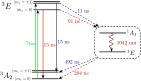
\includegraphics[width=0.8\textwidth]{chapter 1/Figures/ISC}
\caption{Inter system crossing of the NV center. Blue arrows symbolize decay channels to and from the $\ket{m_s=\pm 1}$ states and red arrows the decay channels to and from the $\ket{m_s=0}$ states. Green arrows symbolize the optical excitation induced by the laser. The times indicated correspond to the inverse of the decay rates found in \citep{gupta2016efficient}.}
\label{ISC}
\end{figure}

The optical excitation and radiative decay between the $^3A_2$ and $^3E$ levels preserve the spin projection $m_s$ \citep{robledo2011spin}. There is however a non-radiative decay path which involves in inter-system crossing with the singlet states $^1A_1$ and $^1E$ that depends on the the triplet states spin projection.

Fig. \ref{ISC} summarizes the possible decay channels from the $^3E$ states. We assume that the electrons are initially excited from the $^3A_2$ states via a green laser with a rate $\gamma_{\rm las}$. The $^3E$ states can then either decay radiatevely and emit a 600$-$800 nm photon, or undergo an intersystem crossing and decay through the singlet states. We consider the decay channel through the singlet state as non-radiative due to the strong non radiative channels competing with the IR radiative transition (quantum efficiency $\leq 10^{-3}$ for the singlet transition \citep{rogers2008infrared, ma2010excited, acosta2010optical}).

The rates $\gamma$ of the various decay processes, represented in Fig. \ref{ISC} by the time constant $\tau=1/\gamma$, strongly depends on the spin projection $m_s$: the likeliness to undergo a non-radiative decay is $\sim 4$ times\footnote{$\frac{15+91}{15+11}\approx 4$} more likely when starting from the $\ket{\pm 1}$ states than when starting from the $\ket{0}$ state. Similarly, the singlet state is $\sim 2.4$ times\footnote{$\frac{492}{204} \approx 2.4$} more likely to decay in the $\ket{0}$ state than in the $\ket{\pm 1}$ states.

These spin selective intersystem crossings mean that an optical pumping scheme in the $\ket{m_s=0}$ spin state takes place under constant green excitation. At optical saturation, the polarization of the $\ket{0}$ state can reach $70-90\ \%$ \citep{gupta2016efficient}, which is equivalent to a thermal polarization (for B=0) with a spin temperature of $\approx 65\ \rm mK$ \footnote{\begin{equation*}
T=\frac{h D}{k_B \ln (\frac{1-P}{2P})} \approx 65\ \rm mK,
\end{equation*}
where $D$ is th ZFS factor described in eq. (\ref{eq. spin elec}) and $P\approx 0.8$ is the spin polarization defined as the population in the $\ket{0}$ state.} while the diamond itself can remain at room temperature.

Another effect of the intersystem crossing is the ability to optically readout the spin state of the NV center: since the $\ket{0}$ state is more likely to undergo a radiative decay than the $\ket{\pm 1}$ states, the expected photoluminescence (PL) is higher when starting from the $\ket{0}$ state than a $\ket{\pm 1}$ state. While the $\ket{+1}$ and $\ket{-1}$ states cannot be a priori distinguished, a direct excitation of the $\ket{+1} \to \ket{0}$ or $\ket{-1} \to \ket{0}$ transition with a resonant microwave can unambiguously reveal the initial spin state.

It should be noted that the decay rates indicated in Fig. \ref{ISC} cannot be directly measured. They have to be inferred from the PL dynamics at short times after illumination. Different experiments and different models have thus lead to different decay rates \citep{duarte2021effect}. 


\section{Basic operations with NV centers}

This section introduces two elementary operations with NV centers that are Rabi oscillations and optically detected magnetic resonance (ODMR).

Rabi oscillations is the basis for any kind of coherent qubit manipulation while ODMR is used to find the transition frequencies of the NV centers, as well as being a basic magnetometry protocol.

This section also covers the experimental setup used for these two operations and for many other NV experiments, as well as the concept of longitudinal and transverse magnetic field with regard to the NV principal axis.

\subsection{Experimental setup}
\begin{figure}[h!]
\centering
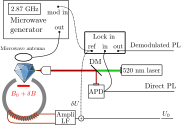
\includegraphics[width=0.8\textwidth]{chapter 1/Figures/shema_exp}
\caption{Confocal microscopy setup detailed in main text}
\label{setup}
\end{figure}
The three most common experimental degrees of freedom to consider for NV experiments are: the optical illumination, the microwave field and the external magnetic field. Other parameters such as the crystal temperature, the electric field or the crystal stress can also be controlled for specific applications.

Fig. \ref{setup} shows a multi-purpose experimental setup which offers a control over these three degree of freedoms. Unless specified otherwise, this is the experimental setup that was used to perform all the measurements shown in this manuscript. 

The setup consists of a confocal microscope where the excitation from a green laser (Thorlabs CPS532, 532 nm, 5 mW) is focused on a sample containing NV centers with a microscope objective (NA $\sim$ 0.5). The NV PL is then collected by the same objective and isolated from the back-scattered laser light with a dichroic mirror (DM) and additional filters (532 nm notch filter and 645 nm longpass filter to filter out the NV$^0$ PL). The PL is collected on an avalanche photodiode (Thorlabs APD410A or Perkin Elmer SPCM-AQRH-15) whose signal is sent to the acquisition card (NI X-series).

The laser beam goes through an acousto-optic modulator (AOM, AA opto-electronic) controlled externally to create arbitrary light pulses (resolution $\sim$ ns). The microwave field is generated by a Rhode \& Shwarz SMB 100A generator and emitted with a home-made loop antenna positioned at $<$ 1 mm of the sample. A microwave switch (Mini-circuits ZASWA-2-50DRA+) is used to create microwave pulses (resolution $\sim$ 10 ns). The control pulses for the AOM and the microwave switch are generated either by the NI X-series card (resolution $\sim$ 1 $\mu$s), or by a pulseblaster ESR-PRO (resolution $\sim$ 10 ns). The microwave field can be amplified with a Mini-circuits ZHL-5W-422+ amplifier to achieve higher Rabi frequencies. 

Finally the magnetic field is generated either with a permanent magnet (up to $\sim$ 200 mT) or with a homemade electromagnet (up to $\sim$ 30 mT) alimented via a low freqency amplifier (Leybold power function generator 522663). Both the permanent magnet and the electromagnet can be  attached to a rotation stage for precise alignment.
\subsection{Rabi Oscillations}
\begin{figure}[h!]
\centering
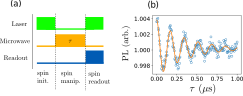
\includegraphics[width=\textwidth]{chapter 1/Figures/Rabi}
\caption{Rabi oscillations. (a) pulse sequence used to measure Rabi oscillations. (b) Experimental data on sample CVD-pink (cf samples [REF]).}
\label{Rabi}
\end{figure}

The general technique for experiments involving NV spins proceeds as follow: 
\begin{itemize}
\item First the spins are polarized. This is done with a green laser pulse ($1-100$ $\mu$s depending on the laser intensity) which polarizes the spins in the $\ket{m_s=0}$ state at $\sim$ 80 \%.
\item  Then the spins are manipulated. This process often involves a microwave field resonant with one of the spin transitions.
\item Finally the spins are read out. The simplest spin readout for NV centers consists in looking at the PL right after the laser is turned on: if the spin was in the $\ket{m_s=0}$ state, the initial PL will be high, whereas if the spin was in a $\ket{m_s=\pm 1}$ state, the initial PL will be low. For longer exposure time, the spins end up re-polarized in the $\ket{m_s=0}$ state and no information can be gained on the initial spin state anymore. The optimal readout time is of the same order as the spin polarization time ($1-100$ $\mu$s).
\end{itemize}

Fig. \ref{Rabi}-a) shows the pulse sequence used to observe Rabi oscillations with NV centers. In this case, the spins manipulation simply consists in a microwave pulse of variable duration $\tau$. The microwave frequency or the magnetic field needs to be adjusted so that at least one NV spin transition (either $\ket{0} \to \ket{+1}$ or $\ket{0} \to \ket{-1}$) is resonant with the microwave field. 

Fig. \ref{Rabi}-b) shows the result of such an experiment on a spin ensemble. The PL signal oscillations correspond to the oscillations of the spin population between the bright $\ket{0}$ state and the dark $\ket{-1}$ state. For long microwave pulses ($>$ 1 $\mu$s typically), the spins reach a steady state with  $\sim$ 50 \% population in both the $\ket{0}$ and $\ket{-1}$ states.


\subsection{Optically detected magnetic resonance}
\begin{figure}[h!]
\centering
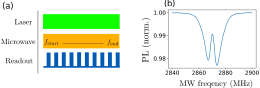
\includegraphics[width=\textwidth]{chapter 1/Figures/ODMR_basique}
\caption{ODMR protocol. (a) Pulse sequence used for CW ODMR: the microwave is kept on during the whole sequence while the frequency is scanned from $f_{\rm start}$ to $f_{\rm end}$. (b) ODMR spectrum with no magnetic field on sample ADM-15-4.}
\label{ODMR basique}
\end{figure}

Optically detected magnetic resonance (ODMR) is the most commonly employed magnetometry protocol with NV centers due to its simplicity and the fact that it does not require prior calibration.

The protocol for continuous wave (CW) ODMR is presented in Fig. \ref{ODMR basique}. In this simple protocol, the microwave is always turned on while the frequency spans a predefined interval $[f_{\rm start}, f_{\rm end}]$. The PL is recorded as the microwave is being swept, with a typical acquisition time for each PL sample $> 1\ \rm ms$. The sweeping frequency must be slow enough so that the PL can reach a steady state with the microwave field for each sample acquisition. 

As we saw in the last section, the steady state of the NV center spin with a resonant microwave field is a statistical mixture of 50 \% $\ket{0}$ and 50 \% $\ket{\pm 1}$ \footnote{We are assuming here that the Rabi frequency is greater than the laser polarizing rate, which is often the case in practice}. If the microwave field is not resonant with a spin transition however, the steady state is predominantly $\ket{0}$ due to the spin polarization caused by the laser. The NV PL will therefore be lowered when the scanning microwave field becomes resonant with one of the NV spin transitions. 

Fig. \ref{ODMR basique}-b) shows an example of ODMR spectrum on an NV ensemble with no external magnetic field. The reason for the two bumps instead of a single one centered on $D=2870\ \rm MHz$ is the splitting of the $\ket{+1}$ and $\ket{-1}$ levels occasioned by the strain and local electric field, which will be further discussed in chapter 4.

\subsubsection{ODMR with lock-in detection}
\begin{figure}[h!]
\centering
\includegraphics[width=\textwidth]{chapter 1/Figures/ODMR_lockin}
\caption{ODMR protocol with lock-in detection. (a) Simplified confocal microscope setup with a lock-in amplifier (LIA) modulating the mircowave and demodulating the PL. (b) Demodulated ODMR spectrum with no magnetic field on sample ADM-15-4.}
\label{ODMR lockin}
\end{figure}


Because the ODMR protocol delivers a continuous signal (the PL) as a function of a periodic excitation (the microwave field), it is well suited to amplitude or frequency modulation and lock-in detection. 

The principle of lock-in detection will not be covered here, the key idea is that lock-in detection allows to translate the signal spectrally in a region less prone to noise. In this case, the ODMR signal is a DC measurement and is therefore prone to slow freqency noises such as thermal or mechanical drifts and laser amplitude fluctuations. The microwave field can thus be modulated (in amplitude, frequency or phase) at a frequency fast enough to mitigate the low freqency noises, but slow enough compared to the NV photodynamics. 

Fig. \ref{ODMR lockin}-a) shows the ODMR lock-in setup, and Fig. \ref{ODMR lockin}-b) shows an example of ODMR spectrum with microwave amplitude modulation. All the lock-in spectra shown in this manuscript were produced with 100 \% amplitude modulation at a frequency $f_{\rm mod} \sim 1\ \rm kHz$.

\subsection{ODMR with NV ensemble: longitudinal and transverse magnetic field}

\begin{figure}[h!]
\centering
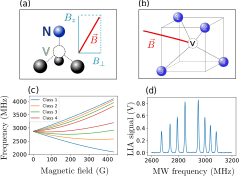
\includegraphics[width=\textwidth]{chapter 1/Figures/ODMR_8_classes}
\caption{(a) Geometry of the NV center and definition of $B_z$ and $B_\perp$. (b) Representation of the 4 possibles orientations (``classes") of the N$-$V axis, corresponding to the 4 $\langle 111 \rangle$ directions of the diamond cubic cell. (c) Simulation of the evolution of the transition frequencies for each class of NV centers as a function of the amplitude of the applied magnetic field ($\textbf{B}$ orientation chosen arbitrarily). (d) ODMR spectrum on sample ADM-150-1 for a magnetic field of $\sim 90\ \rm G$.}
\label{ODMR 8 classes}
\end{figure}

We mentioned previously that the NV spin Hamiltonian (eq. (\ref{NV spin Hamiltonian basic})) was anisotropic due to the fine structure term $D S_z^2$ where $z$ is the direction of the N$-$V axis in the crystal. The magnetic field is thus often decomposed between the longitudinal magnetic field $B_z$ and the transverse magnetic field $B_\perp=\sqrt{B_x^2+B_y^2}$ (see Fig. \ref{ODMR 8 classes}-a). 

For weak magnetic fields ($\gamma |\textbf{B}| \ll D$), the energy of each of the three spin Hamiltonian eigenstates $\ket{0}$, $\ket{+1}$ and $\ket{-1}$\footnote{The notation of $\ket{0}$, $\ket{\pm 1}$ to designate the spin Hamiltonian eigenstates is slightly abusive as $S_z$ does not commute with $\mathcal{H}$ when $B_\perp \neq 0$. The true eigenstates however remain close to $\ket{0}$, $\ket{\pm 1}$ as long as $\gamma_e B_z > \frac{(\gamma_e B_\perp)^2}{D}$.} can be approximated in a perturtbative approach to: %cf AN.py
\begin{align}
\nu_0&= -\frac{(\gamma_e B_\perp)^2}{D} \\
\nu_{-1} &= D - \gamma_e B_z + \frac{(\gamma_e B_\perp)^2}{2D} \\
\nu_{+1} &= D + \gamma_e B_z + \frac{(\gamma_e B_\perp)^2}{2D}
\end{align}

Fig. \ref{ODMR 8 classes}-b) represent the 4 possible orientation of the N$-$V axis in a diamond single crystal. We refer to these orientations as ``classes" since NV centers belonging to the same class will perceive the same transverse and longitudinal magnetic field, and thus will have the same spin Hamiltonian. For large NV ensembles (a confocal spot can contain more than $10^9$ NV centers in dense ensemble), we can consider that each class is equally represented \footnote{It is possible to create NV centers with a preferential orientation \citep{lesik2014perfect} but this requires specific conditions during the growth process of the diamond} and that each class is responsible for two lines in the ODMR spectrum (one for the $\ket{0} \to \ket{-1}$ transition and one for the $\ket{0} \to \ket{+1}$ transition). 

Fig. \ref{ODMR 8 classes}-c) shows a simulation of the evolution of the transition frequencies $\nu_{+1} - \nu_{0}$ and $\nu_{-1} - \nu_{0}$ for all 4 classes as a function of the magnetic field amplitude, with the magnetic field orientation fixed in an arbitrary direction. Fig. \ref{ODMR 8 classes}-d) shows an ODMR spectrum with NV ensembles. 8 lines are visible corresponding to the two transitions of the 4 classes. Based on the position of these 8 lines, it is possible to determine the projection of the magnetic field on each of the 4 N$-$V axes, and thus to reconstruct the full 3D magnetic field with respect to the diamond crystalline axes.

We should also note that the state mixing caused by the transverse magnetic field deteriorates the polarization scheme detailed in Sec. \ref{sec ISC}. For strong transverse magnetic fields ($\gamma_e B_\perp \sim D$), the optical polarization is almost completely quenched, which prevents any kind of coherent NV manipulation \citep{tetienne2012magnetic}.

\section{Dynamics of the NV center spin}

This section focuses on the dynamics of the NV spin, and more specifically on its various relaxation times. Relaxation times are important properties of spin qubits as they often are the limiting factor for quantum information or quantum sensing applications \citep{de2021materials, degen2017quantum}.

The relaxation times are generally decomposed between the longitudinal relaxation time $T_1$ which corresponds to the characteristic time of the return to thermal equilibrium for the populations (diagonal elements of the density matrix), and the transverse relaxation time $T_2$\footnote{We follow here the NMR nomenclature} which corresponds to the relaxation of the spin state coherences (non diagonal elements of the density matrix).

The transverse relaxation time, also called coherence time or dephasing time, is often further decomposed between the inhomogeneous dephasing time $T_2^*$ and the homogeneous dephasing time $T_2$. The $T_2^*$ time includes inhomogeneous dephasing processes such as the inhomogeneity in space (when multiple qubits are probed) and time of the external fields. The $T_2$ time corresponds to the coherence time where some of these inhomogeneities have been corrected, for instance with a Hanh echo sequence \citep{hahn1950spin} or a dynamical decoupling scheme \citep{naydenov2011dynamical}. While $T_2^*$ is an intrinsic property of the sample studied, $T_2$ depends on the rephasing scheme used. More careful nomenclatures will label the $T_2$ times as $T_{2,\rm echo}$ or $T_{2,\rm DD}$ \citep{de2021materials} for instance. The relaxation times are ordered as follows:
\begin{equation}
T_2^* < T_2 < 2 T_1.
\end{equation}

The relaxation times of NV centers depend mainly on their environment, and can vary by several order of magnitude depending on the sample used. The following paragraphs will cover the measurement processes of the different relaxation times and the typical values for the samples used in this manuscript.

\subsection{NV spin $T_1$}
\label{sec T1 NV}
\subsubsection{Measurement protocol}
\begin{figure}[h!]
\centering
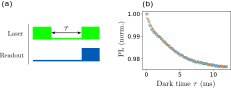
\includegraphics[width=\textwidth]{chapter 1/Figures/T1_basique}
\caption{Basic $T_1$ measurement scheme. (a) Pulse seqeunce used. (b) Experimental data obtained on sample CVD-pink for low laser intensity. The orange line corresponds to an exponential fit with time constant $\tau=4.0\ \rm ms$.}
\label{T1 basique}
\end{figure}


$T_1$ is the simplest relaxation time to measure because the spin populations are directly correlated to the NV centers PL. Fig. \ref{T1 basique} shows the pulse sequence used and an experimental result of the $T_1$ sequence. The spin lifetime $T_1$ is one of the only spin property that can be measured without a resonant microwave.

The sequence shown in Fig.\ref{T1 basique} can be improved by implementing a common mode rejection technique described in Fig. \ref{T1 soustraction}-a). This protocol works as follow: first, a basic $T_1$ sequence is recorded, which we will denote $S_1$. Then the sequence is repeated with an additional $\pi$-pulse on one the NV transitions right before the readout. This $\pi$-pulse will project the remaining $\ket{0}$ population difference into a $\ket{\pm 1}$ state. The second readout is labeled $S_2$, and the final spin state readout is $S_1 -S_2$ which rejects every contribution to the PL outside of the spin relaxation. 



Fig. \ref{T1 soustraction}-b) shows the experimental result of the $S_1$ and $S_2$ sequences on the same sample that was used in Fig. \ref{T1 basique}. The difference between the $S_1$ data in Fig. \ref{T1 soustraction}-b) and the the data in Fig. \ref{T1 basique}-b) comes from the laser intensity used. In Fig. \ref{T1 soustraction}, the laser intensity was high enough ($> 1\ \rm{mW}$) that photoionization between NV$^-$ and NV$^0$ becomes significant. Furthermore, for dense ensemble, a charge recombination mechanism operates even in the dark \citep{giri2018coupled, giri2019selective} (most likely due to charge tunneling between impurities \citep{choi2017depolarization}) . On the other hand, the laser intensity used in Fig. \ref{T1 basique} was small enough ($< 10\ \mu \rm{W}$) that the charge state state photodynamics contribution was negligible compared to the spin depolarization.

Fig. \ref{T1 soustraction}-c) Shows the subtraction of the $S_1$ and $S_2$ signal. Despite the complex shape of the initial $S_1$ and $S_2$ signals, $S_1-S_2$ is nicely fitted with an exponential decay similar to the results found in Fig. \ref{T1 basique}.

\begin{figure}[h!]
\centering
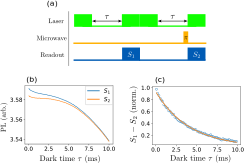
\includegraphics[width=\textwidth]{chapter 1/Figures/T1_protocole_soustraction}
\caption{Common mode rejection $T_1$ measurement scheme. (a) Pulse seqeunce used. (b) PL signals $S_1$ and $S_2$ obtained on sample CVD-pink with a high laser intensity. (c) Subtraction $S_1-S_2$ versus dark time $\tau$. The experimental data is fitted with an exponential decay of time constant $\tau=4.1\ \rm ms$.}
\label{T1 soustraction}
\end{figure}

The photodynamics of the NV charge state is a complex subject which is still actively researched \citep{craik2020microwave, gorrini2021long}. The common mode rejection scheme described  here is often employed with dense ensemble of NV centers \citep{jarmola2012temperature, mrozek2015longitudinal, choi2017depolarization} as it allows to completely bypass the charge dynamics.

\subsubsection{Physical origin and typical values}

We distinguish three different origin for the the $T_1$ relaxation process:
\begin{itemize}
\item \textbf{Spin-phonon relaxation:} the spin states are weakly coupled to the crystal phonon bath through spin-spin and spin-orbit interactions \citep{norambuena2018spin}, which can result in a phonon-induced spin relaxation. The dominant relaxation mechanism depends on the  temperature regime, with the two-photon Raman process believed to be dominant at room temperature \citep{takahashi2008quenching, jarmola2012temperature} while the dominant process as at cryogenic temperature ($4\sim100$ K) is believed to be a two phonons Orbach process \citep{redman1991spin, norambuena2018spin}. The spin-phonon relaxation time strongly depends on the crystal lattice temperature, with relaxtion times of the order $T_1 \sim 5\ \rm ms$ at room temperature, and up to 8 hours at for mili-K temperatures \citep{astner2018solid}.

\item \textbf{Electric and magnetic field noises:} both electric and magnetic fields can directly excite the $\ket{0} \to \ket{\pm 1}$ spin transition \citep{udvarhelyi2018spin}. As a result, magnetic and electric field noise can reduce the spin $T_1$ if their spectrum overlap with the NV transitions. This is particularly important for near surface spins because of the strong noise caused by electronic defects on the surface \citep{sangtawesin2019origins}. The $T_1$ of near surface NV center can be as low as $\sim 10\ \mu$s, but the surface effects are only effective at very short range (within $\sim 10\ \rm nm$ of the surface).

\item \textbf{Resonant dipolar interaction with other paramagnetic impurities:} Dipolar interaction betwen two spins will be detailed more thoroughly in the following section. Dipole-dipole interaction between NV centers and surrounding spins is responsible for both transverse and longitudinal spin relaxation, with the added condition of energy matching (resonance) for longitudinal relaxation. The $T_1$ time associated with dipole-dipole interaction strongly depends on the spin concentration and can be as low as $\sim 25 \mu$s \citep{hall2016detection}.
\end{itemize}

All the measurements shown in this manuscript were performed at room temperature. The spin-phonon interaction thus creates a baseline value for the NV $T_1$ time at $\sim 5\ \rm ms$. Every sample studied were at least a few $\mu$m thick and we will therefore neglect the surface noise contribution in our analyses. The dipole-dipole induced relaxation however is of crucial importance for the next chapters, where it will be further detailed. $T_1$ times between $0.1 \sim 1\ \rm ms$ were routinely observed for samples with high NV concentration.

\subsection{NV spin $T_2^*$}
\subsubsection{Measurement protocol}
\begin{figure}[h!]
\centering
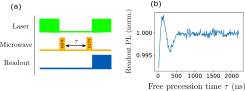
\includegraphics[width=\textwidth]{chapter 1/Figures/Ramsey}
\caption{Ramsey interferometry protocol. (a) Pulse seqeunce used. (b) Experimental data obtained on sample CVD-pink.} %The orange line corresponds to an Gaussian fit with time constant $\tau=400 \pm 100\ \rm ns$.}
\label{Ramsey}
\end{figure}

The $T_2^*$ time is the characteristic time for the loss of quantum coherence of a freely evolving system. It is generally defined as the decay time of of a Ramsey interferometry measurement \citep{barry2020sensitivity}.

Fig. \ref{Ramsey} shows the Ramsey pulse sequence and an  example obtained on a spin ensemble. The microwave frequency is detuned by $\sim 300\ \rm kHz$ compared to the spin central Larmor frequency which causes oscillations in the signal. $T_2^*$ is the decay time of the envelope of the Ramsey fringes. Unfortunately, it is hard to correctly fit the envelope of a signal with so few fringes. Increasing the number of fringes with our current microwave and optical setup might prove hard, as further microwave detuning would decrease the signal contrast, and would be ultimately limited by the microwave pulses resolution.

Ramsey sequences are generally harder to perform on NV ensemble than they are on single NV for two main reasons. The first one is that the $T_2^*$ times tend to be longer for single NV centers as they do not suffer from spatial inhomogeneity, and because the samples used for single NV experiments generally contains less impurities than those used for NV ensemble. The second one is the inhomogeneous microwave power which leads to a variation of the Rabi frequencies among the spins \citep{barry2016optical, zhou2020quantum} and lowers the fringe contrast.

An alternative measurement of $T_2^*$ can be performed by looking at the linewidth of an ODMR spectrum. Indeed, ideally the ODMR spectrum should be the Fourier transform of the Ramsey signal (also called free induction decay in NMR literature). In practice however, both methods suffer from experimental noises and imperfections, with Ramsey-type methods being more sensitive to microwave inhomogeneities \citep{barry2020sensitivity} while ODMR is prone to laser and microwave power broadening \citep{dreau2011avoiding}. 

The method chosen to extract $T_2^*$ values in this manuscript was ODMR with low microwave power ($\Omega_{\rm Rabi} \ll 1/T_2^*$) and low laser intensity (compared to the the NV optical saturation).

\subsubsection{Physical origin}

\begin{figure}[h!]
\centering
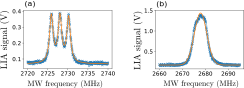
\includegraphics[width=\textwidth]{chapter 1/Figures/ODMR_1_classes}
\caption{ODMR spectra on a single NV class. (a) Experimental data on sample CVD-pink, fitted with three Lorentzians with HWHM $530$ kHz ($T_2^*=300\ \rm ns$). (b) Experimental data on sample Sumi-2, fitted with a single Gaussian with HWHM $3.2$ MHz ($T_2^*=83 ns$).}
\label{ODMR 1 classe}
\end{figure}

For most samples, the leading cause of inhomogeneous dephasing is the temporal and spatial variations of magnetic fields caused by the paramagnetic impurities in the crystal \citep{barry2020sensitivity}. The nature of these different paramagnetic impurities will be further discussed in the section dedicated to dark spins in diamond in chapter 2. We will simply mention here that for sample with high NV density ([NV] $\geq$ ppm), $T_2^*$ is mostly limited by the electronic spins of nitrogen impurities \citep{bauch2018ultralong}.

Fig. \ref{ODMR 1 classe} shows ODMR spectra of a single NV class on two distinct samples (see [REF]). The first sample is a CVD sample with a total substitutional nitrogen  concentration $[N_s] \approx 26\ \rm ppm$, while the second is a type-Ib HPHT sample with a likely nitrogen concentration $[N_s] \geq 100\ \rm ppm$. We can clearly see a higher linewidth, corresponding to a smaller $T_2^*$ value on the sample with higher nitrogen concentration. In particular, we can notice the hyperfine structure of the $^{14}$N nuclei on the CVD sample, whereas it is hidden by the inhomogeneous broadening on the HPHT sample.

Fig. \ref{ODMR 1 classe} illustrates another difficulty of $T_2^*$ measurement which is to find the correct fitting formula. While the spectral profile of single NV centers is expected to be Gaussian, the spectral profile of an ensemble of NV centers  is expected to be Lorentzian \citep{dobrovitski2008decoherence, hall2014analytic}. For Fig. \ref{ODMR 1 classe}-a), it was indeed found that Lorentzians fitted the data better than Gaussians. For Fig. \ref{ODMR 1 classe}-b) however, a Gaussian was found to be a better fit than a Lorentzian, although this could be in part due to the unresolved hyperfine structure.

\subsection{NV spin $T_2$}
\begin{figure}[h!]
\centering
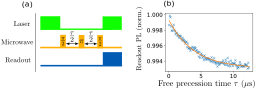
\includegraphics[width=\textwidth]{chapter 1/Figures/Echo}
\caption{Spin-echo protocol. (a) Pulse seqeunce used. (b) Experimental data obtained on sample CVD-pink, fitted with an exponential decay of time $3.9\ \rm{\mu s}$.} 
\label{Echo}
\end{figure}
\subsubsection{Measurement protocol}
As precised earlier, the exact $T_2$ definition depends on the rephasing scheme used. We will focus here on the simplest known rephasing process which is the spin-echo or Hahn-echo sequence.

Fig. \ref{Echo} shows the pulse sequence used and an example on the same sample than the Ramsey measurement. The pulse sequence differs from the Ramsey one by adding a a $\pi$-pulse in the middle of the free precession time. This additional $\pi$-pulse causes static or slowly varying dephasing to be rephased \citep{hahn1950spin}. 

This protocol extends the coherence time on this particular sample from $T_2^* \approx 300\ \rm ns$ to $T_2 \approx 4\ \rm{\mu s}$, an increase by more than a factor of 10. Improvement by a factor of $10 \sim 100$ or typical for NV ensembles \citep{barry2020sensitivity}. This value could likely be extended even further by using a more complex dynamical decoupling scheme from the CPMG or XY sequence families \citep{naydenov2011dynamical, bar2012suppression}.

\subsubsection{Physical origin}
The origin of the relaxation time $T_2$ are fluctuating noises which are too fast to be efficiently rephased by the sequence. The origin of these noises is generally attributed to the flipping of spins in the vicinity of the NV center (either through spin-lattice or spin-spin mechanisms) \citep{hall2014analytic}. For samples with high nitrogen concentration, it has been measured that the $T_2$ time  was directly correlated to the nitrogen concentration, with the same scaling than the $T_2^*$ time \citep{bauch2019decoherence}.

\section{Dipole-dipole interaction between two electronic spins}

\begin{figure}[h!]
\centering
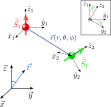
\includegraphics[width=0.4\textwidth]{chapter 1/Figures/shema_dipole_dipole}
\caption{Geometric representation of two interacting spins. ($\mathbf{x}_1,\mathbf{y}_1,\mathbf{z}_1$) and ($\mathbf{x}_2,\mathbf{y}_2,\mathbf{z}_2$) represent Cartesian coordinate systems in the spin frames of reference, where $\mathbf{z}_i$ is the axis of quantization of spin $i$.} 
\label{dipole-dipole}
\end{figure}

This final introductory section will focus on the dipole-dipole interaction between two electronic spins, which is the main form of spin-spin interaction and plays a key part in the properties of dense spin ensemble. 

We will consider the general situation represented in Fig. \ref{dipole-dipole}: two spins separated by a distance $r$ with their own coordinate systems ($\mathbf{x}_1,\mathbf{y}_1,\mathbf{z}_1$) and ($\mathbf{x}_2,\mathbf{y}_2,\mathbf{z}_2$). The coordinate system is chosen so that each spin operator can be written:

\begin{equation}
\hat{\mathbf{S}}_i=\hat{S}_x \mathbf{x}_i + \hat{S}_y \mathbf{y}_i + \hat{S}_z \mathbf{z}_i
\end{equation}

where the spin operators $\hat S_{\{x,y,z\} }$ have their usual definitions in term of Pauli matrices. In particular, this means that the spin axis of quantization of each spin is $z_i$, which classically corresponds to the magnetization direction of the dipole. This axis can be defined either by the magnetic field, or by crystal field anisotropies, as is often the case for solid state spins with $S\geq 1$ (including the NV center).

\subsection{Magnetic dipole-dipole Hamiltonian}

Classically, the dipole-dipole interaction between two magnetic moments $\mathbf{m}_1$ and $\mathbf{m}_2$ can be derived by computing the static magnetic field generated by one dipole at the position of the second dipole \cite[p.~188]{jackson1999classical}:

\begin{align}
U&=-\mathbf{m}_1 \cdot \mathbf{B}(\mathbf{r}) \nonumber \\
&=-\frac{\mu_0}{4 \pi}\left[ \frac{3 (\mathbf{m}_1\cdot\mathbf{u})(\mathbf{m}_2\cdot\mathbf{u}) - \mathbf{m}_1\cdot\mathbf{m}_2}{r^3}+\frac{8\pi}{3}\mathbf{m}_1\cdot\mathbf{m}_2\,\delta(r)\right], \label{eq. dipole classique}
\end{align}

where $\mathbf{r}=r \mathbf{u}$ is the relative position of the two dipoles (see Fig. \ref{dipole-dipole}). 

The quantum analog of the dipole-dipole interaction between spins simply replaces the magnetic moments $\mathbf{m}_i$ in eq. (\ref{eq. dipole classique}) with $\hbar \gamma_i \hat{\mathbf{S}}_i$, where $\gamma_i$ is the gryromagnetic ratio and $\hat{\mathbf{S}}_i$ the spin vector operator for spin $i$:

\begin{equation}
\mathcal{H}_{\rm dd}=\frac{\mu_0 \gamma_1 \gamma_2 \hbar^2}{4 \pi}\left[ \frac{3 (\hat{\mathbf{S}}_1\cdot\mathbf{u})(\hat{\mathbf{S}}_2\cdot\mathbf{u}) - \hat{\mathbf{S}}_1\cdot\hat{\mathbf{S}}_2}{r^3}+\frac{8\pi}{3}\hat{\mathbf{S}}_1\cdot\hat{\mathbf{S}}_2\,\delta(r)\right].
\end{equation}

The $\delta(r)$ term represents the Fermi contact energy. This term plays an important role when there is an overlap of the spin particle wavefunctions, such as the hyperfine coupling between the NV$^-$ electron spin and $^{14}$N \cite{doherty2012theory} or  $^{13}$C \cite{smeltzer201113c} nuclear spins.

The focus of this manuscript is on the interaction between electronic spins which are separated by several atomic sites (density impurities in the $\sim$ ppm range). We will therefore assume that there is negligible overlap between the electronic wavefunctions and omit the Fermi contact term. This leads the simplified dipole-dipole Hamiltonian:

\begin{equation}
\mathcal{H}_{\rm dd}= \frac{J_0}{r^3}\left[ 3 (\hat{\mathbf{S}}_1\cdot\mathbf{u})(\hat{\mathbf{S}}_2\cdot\mathbf{u}) - \hat{\mathbf{S}}_1\cdot\hat{\mathbf{S}}_2] \right],
\end{equation}

where $J_0=\frac{\mu_0 \gamma_1 \gamma_2 \hbar^2}{4 \pi}$.

For two electronic spins with $g$-factors $\approx -2$\footnote{Most spin defects in diamond, including the NV center have a g-factor $\approx -2$ similarly to free electrons.}, 
\begin{equation*}
\frac{J_0}{h} \approx 51.8\ \rm{MHz}\cdot \rm{nm}^3.
\end{equation*}

\subsection{Decomposition of the dipole-dipole Hamiltonian}

\begin{figure}[h!]
\centering
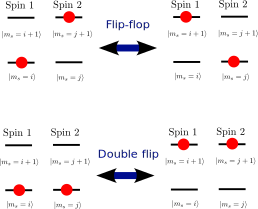
\includegraphics[width=.7\textwidth]{chapter 1/Figures/flip-flop_double-flip}
\caption{Representation of the two energy transfer mechanisms: flip-flop and double flips} 
\label{flip flop double flip}
\end{figure}

In the weak coupling approximation, the dipole-dipole Hamiltonian between two spins can be decomposed between diagonal terms which are responsible for energy shifts of the individual spin levels, and the off-diagonal terms which are responsible for energy transfers between the two spins.

In what follows, we will assume that both spins have the same quantization axis in order to simplify the Hamiltonian decomposition. A more general case is detailed in [REF].

Following the notation introduced in Fig. \ref{dipole-dipole}, we will then assume that $$(\mathbf{x}_1,\mathbf{y}_1,\mathbf{z}_1) = (\mathbf{x}_2,\mathbf{y}_2,\mathbf{z}_2) = (\mathbf{x},\mathbf{y},\mathbf{z}).$$ We will denote $\mathbf{u}=u_x \mathbf{x} + u_y \mathbf{y} + u_z \mathbf{z}$ the decomposition of the unitary vector $\mathbf{u}$ in this basis. The dipole-dipole Hamiltonian can then be written:
\begin{equation}
\mathcal{H}_{\rm dd}=\frac{J_0}{r^3}\left[ (3 u_x^2-1) S_x^1 S_x^2 + (3 u_y^2-1) S_y^1 S_y^2 + (3 u_z^2-1) S_z^1 S_z^2 \right],
\end{equation}
where $S_{\{x,y,z\} }^i$ are the spin operators acting on spin $i$. The $S_z^1 S_z^2$ term is the only diagonal term and corresponds to energy shifts while the $S_x^1 S_x^2$ and $S_y^1 S_y^2$ terms are responsible for energy transfer. To make the transfer mechanism more apparent, we will rewrite $S_x^i$ as $\frac{1}{2}(S_+^i+S_-^i)$ and $S_y^i$ as $\frac{1}{2i}(S_+^i-S_-^i)$:
\begin{align}
\mathcal{H}_{\rm dd}&=\frac{J_0}{r^3}\bigg{[} \frac{1}{4}(3 u_x^2 + 3 u_y^2 -2)(S_+^1 S_-^2 + S_-^1 S_+^2) \nonumber \\
&\quad + \frac{1}{4}(3 u_x^2 - 3 u_y^2)(S_+^1 S_+^2 + S_-^1 S_-^2) \nonumber \\
&\quad +(3 u_z^2-1) S_z^1 S_z^2 \bigg{]} \nonumber \\
\medskip
&= \Omega_{\rm ff} (S_+^1 S_-^2 + S_-^1 S_+^2) + \Omega_{\rm df} (S_+^1 S_+^2 + S_-^1 S_-^2) + \Omega_{\rm shift} S_z^1 S_z^2. \label{eq. ff df}
\end{align}

We have introduced in eq. (\ref{eq. ff df}) the three relevant matrix elements $\Omega_{\rm ff}$, $\Omega_{\rm df}$, and $\Omega_{\rm shift}$ which correspond respectively to flip-flops, double flips and energy shifts. Flip-flops and double flips (sometimes referred as flip-flips) are represented in Fig. \ref{flip flop double flip}. Flip flops correspond to energy transfer between two spins for which the sum of the spin angular momentum is conserved ($\Delta (m_s^1+m_s^2)=0$), while double flips correspond to energy transfer for which the spin angular momentum is not conserved ($\Delta (m_s^1+m_s^2)=\pm 2$)\footnote{In order to preserve the total angular momentum, double flips transfer angular moment to the crystal, which is a form of Einstein de Haas effect \citep{einstein1915experimental} }. In both cases however, the energy between the initial and final states needs to be preserved for the transfer to be efficient. 

It should be noted that on average, each matrix element is of the same order of magnitude: $\Omega_{\rm ff} \sim \Omega_{\rm df} \sim \Omega_{\rm shift} \sim \frac{J_0}{r^3}$. 

\subsection{Cross-relaxations with NV centers}

\begin{figure}[h]
\centering
\includegraphics[width=0.9\textwidth]{chapter 1/Figures/Shema_CR}
\caption{Illustration of cross-relaxations between an NV center and an unpolarized spin. Red dots represent the population in each states, and the arrows the various population transfer mechanisms}
\label{CR_shema}
\end{figure}

Cross-relaxation (CR) is the transfer of polarization from one spin to another (or more generally from one family of spins to another family). This process can occur through either flip-flops or double flips, as long as the resonance condition between the two spins is met. 

On of the condition for cross-relaxation is to have a difference in polarization between the two spins species considered. The NV center is therefore a good candidate to observe cross-relaxations as it can be optically polarized while most other spin species are not. 

Fig. \ref{CR_shema} illustrates CR between a polarized NV center and an unpolarized second spin. When the two considered spin transitions become resonant, in this case by tuning the magnetic field, polarization from the NV center will be transferred to the second spin, making the NV center less polarized and the second spin more polarized than when they are out of resonance. 

For a single NV center coupled to spin 2, assuming that spin 2 always remains depolarized\footnote{This is the case in practice if the spin 2 bath is much bigger than the NV bath and effectively acts as a thermostat, or if the lifetime of spin 2 is much smaller than that of the NV center.} and that the coupling strength between the two spins is smaller than their respective dephasing time $T_2^*$ (weak coupling regime), the modification in the NV relaxation rate $\Gamma_1=\frac{1}{T_1}$ caused by the cross-relaxation with spin 2 can be analytically computed \citep{hall2016detection}:
\begin{equation}
\delta \Gamma_1=\frac{\Omega^2}{\Gamma_2^*} \frac{(\Gamma_2^*)^2}{(\delta \nu)^2+(\Gamma_2^*)^2},
\label{delta gamma 1}
\end{equation}
where $\Gamma_2^*=\frac{1}{T_2^*(\rm NV)}+\frac{1}{T_2^*(\rm Spin 2)}$ is the joint dephasing rate of the NV center and the second spin, $\delta \nu$ is the detuning in energy (expressed in frequency) between the initial and final states and $\Omega=\Omega_{\rm ff}$ or $\Omega_{\rm df}$ is the dipole-dipole matrix element corresponding to the flip-flop or double-flip process considered. 

Eq. (\ref{delta gamma 1}) is the basis for every cross-relaxation detection performed in this manuscript. Because the NV center lifetime can be measured optically, as detailed in Sec. \ref{sec T1 NV}, cross-relaxation between NV-centers and other spin species can be measured optically. Measuring the cross-relaxation depolarization can then be used to gain information on the second spin or on the dipole-dipole interaction mechanisms, as will be explained in the following chapters.

\section{Conclusion}

We have covered in this introductory chapter every concepts needed to understand the results presented in the next chapters. We have seen the main steps in the creation of artificial diamonds and NV centers, we have covered the optical and spin properties of the NV center as well as the ways to measure them, and we have introduced the notion of dipole-dipole coupling and cross-relaxation between two spins.

The focus of chapter 2 will be on the cross-relaxation between NV centers and other spin impurities in CVD-grown diamond, while the focus of chapter 3 and 4 will be on the cross-relaxation between NV centers and other NV centers, as well as their potential application in magnetometry.
\printbibliography
\end{refsection}
 \begin{refsection}

\chapter{Detection of dark spins via cross-relaxations}
In this chapter, we will see how the interplay between the optical and spin properties of the NV centers can be transferred to other spins in the crystal by coupling them to NV centers. More specifically, I will discuss the first optical detection of two spin species, VH$^-$ and War1, in a CVD diamond by the mean of cross-relaxations with NV centers.
\section{Flip-Flops, double flips and cross-relaxation}
\label{Sec_CR}

\subsection{Resonant interaction : flip-flops and double flips}

The dominant form of interaction between two distant spins is the magnetic dipole-dipole interaction. For two spins with with vector spin Hamiltonian $\hat{\mathbf{S}}_1$ and $\hat{\mathbf{S}}_2$, separated by a distance $\mathbf{r}=r\mathbf{u}$, the dipole-dipole interaction Hamiltonian reads (see Appendix A) :
\begin{equation}
\mathcal{H}_{dd}=\frac{J_0}{r^3}\left[ \hat{\mathbf{S}}_1\cdot\hat{\mathbf{S}}_2 - 3 (\hat{\mathbf{S}}_1\cdot\mathbf{u})(\hat{\mathbf{S}}_2\cdot\mathbf{u})\right],
\end{equation}
where $J_0= \frac{\mu_0\gamma_1\gamma_2 \hbar^2}{4\pi}$. For two electronic spins with $g-$factors close to 2 (which is the case for the NV center and most spin defect in diamond), the numerical value of $J_0$ is $(2\pi)\,52\ \rm{MHz}\cdot\rm{nm}^3$.

Flip-flop, in the context of dipole-dipole interaction, is the mechanism which exchanges a quantum of spin between two spins. For an initial state of two spins $\ket{m_s^1=i;m_s^2=j}$, a flip-flop process will result in a final state $\ket{i+1;j-1}$ or $\ket{i-1;j+1}$. The effective rate of this process depends on the matrix element $\mel{i;j}{\mathcal{H}_{dd}}{i\pm 1;j \mp 1}$, as well as the resonance condition between the initial and final state. We should note that for two identical spins, the flip-flop process $\ket{i;i\pm 1}\bra{i\pm 1,i}$ is always resonant.

Another mechanism authorized by the dipole-dipole Hamiltonian is the double-flip, either up or down, which couple the states $\ket{i;j}$ and $\ket{i-1;j-1}$ or $\ket{i+1;j+1}$. For a single spin species in a strong magnetic field, the lift of the various spin levels by the Zeeman effect means that no double-flip process can be resonant. However with weak magnetic field or when two different spin species are present, double flip process can be as important as flip-flops since the matrix elements $\mel{i;j}{\mathcal{H}_{dd}}{i\pm 1;j \pm 1}$ are typically of the same order of magnitude as the flip-flop ones.

\subsection{Cross-relaxations}

\begin{figure}[h]
\centering
\includegraphics[width=0.9\textwidth]{chapter 2/Figures/Shema_CR}
\caption{Illustration of cross-relaxations between an NV center and an unpolarized spin. Red dots represent the population in each states, and the arrows the various population transfer mechanisms}
\label{CR_shema}
\end{figure}

Cross-relaxation (CR) is the transfer of polarization from one spin to another (or more generally from one family of spins to another family). This process con occur either through flip-flops, or through double flips, as long as the resonance condition between the two spins is met. 

Fig. \ref{CR_shema} illustrates CR between a polarized NV center and an unpolarized second spin. When the two considered spin transitions become resonant, in this case by tuning the magnetic field, polarization from the NV center will be transferred to the second spin, making the NV center less polarized and the second spin more polarized than when they are out of resonance. 

The reason why CR tend to depolarize the NV center simply comes from a rate equation : since the initial NV population is higher in the $\ket{0}$ state than in the $\ket{-1}$ state, the flip-flop (or double flip) process that makes the NV center go to $\ket{-1}$ (symbolized by the two red arrows in Fig. \ref{CR_shema}) is more likely than the reverse flip-flop. If we only focus on the NV center, cross-relaxation is simply another thermalization process due to the coupling of the NV center to its environment.

For a single NV center coupled to spin 2, assuming that spin 2 is initially depolarized and that the coupling strength between the two spins is smaller than their respective dephasing time $T_2^*$, we can compute the modification in the NV relaxation rate $\Gamma_1=\frac{1}{T_1}$ caused by spin 2 as \citep{hall2016detection}:
\begin{equation}
\delta \Gamma_1=\frac{\Omega^2}{\Gamma_2^*} \frac{(\Gamma_2^*)^2}{(\delta \nu)^2+(\Gamma_2^*)^2},
\label{delta gamma 1}
\end{equation}
where $\Omega=\frac{\mel{i;j}{\mathcal{H}_{\rm dd}}{j;i}}{\hbar}$ is the matrix element of the dipole-dipole Hamiltonian that couples the initial and final states, $\Gamma_2^*=\frac{1}{T_2^*(\rm NV)}+\frac{1}{T_2^*(\rm Spin 2)}$ is the joint dephasing rate of the NV center and the second spin, and $\delta \nu$ is the detuning between the central frequencies of the NV center and spin 2.
\section{The dark spins in diamond}

We refer by dark spins to spin defects which do not interact with light, which in the case of diamond defects consist of almost every known spin defect bar the NV center and the more recently found ST1 center \citep{lee2013readout, john2017bright}.

\subsection{P1 centers and $^{13}$C}
By far the most common spin defects in NV-rich diamond, outside of NV centers, are the substitutional nitrogen centers N$^0_S$ known as the P1 centers, which have an electronic spin $1/2$ and a nuclear spin 1, and the $^{13}$C $1/2$ nuclear spin which is present at 1.1\% in natural abundance carbon, the remaining carbon atoms being almost exclusively the spinless $^{12}$C isotope. 

In NV-rich diamonds, these two impurities are the main causes of the inhomogeneous dephasing rate $\Gamma_2^*=1/T_2^*$ of the NV centers ensemble \citep{barry2020sensitivity}. The dephasing comes from the distribution of dipole-dipole coupling from each NV centers to its neighboring spin defects, which varies in space and time. 

The dephasing rate caused by a given impurity is directly proportional to the diagonal dipole-dipole matrix elements \citep{bauch2020decoherence}: 
\begin{equation}
\Gamma_2^*(\rm P1) \propto \Omega_{\rm NV-P1}=\frac{1}{\hbar}\sqrt{\sum_j \abs{\mel{NV=i;P1=j}{\mathcal{H}_{\rm dd}}{NV=i;P1=j}}^2}.
\label{Gamma2 P1}
\end{equation}
Since the dipole-dipole coupling rate scales as $1/r^3$, and the distance $r$ between each spin scales as the inverse cubic root of the concentration,  it is expected that the dephasing rate associated with a particular impurity scales linearly with the concentration of the impurity: $\Gamma_2^*(\rm P1) \propto [P1]$. In the case of P1 centers, this was verified experimentally by \citep{bauch2020decoherence} who found a value of $\Gamma_2^*(\rm P1)= (2 \pi) 16\ \rm kHz/ppm$. The typical concentrations of P1 center go from [REF] for high purity CVD diamond, up to 500 ppm for type 1B HPHT or natural diamonds.

$^{13}$C is much more abundant than P1 center ($\sim$ 10 000 ppm at natural abundance) but being a nuclear spin, it has a gyromagnetic ratio $\approx 2.8\cdot 10^3$ times smaller than that of the P1. This results in a contribution to $\Gamma_2^* \sim 10^3$ times smaller per impurity. It was found experimentally that the broadening caused by $^{13}$C is $\Gamma_2^*(^{13}\rm C ) \approx (2 \pi) 16\ \rm Hz/ppm$ \citep{van1997dependences, barry2020sensitivity}. For natural abundance diamond, this means that $\Gamma_2^*(^{13}\rm C ) \approx (2 \pi) 160\ \rm kHz$.

\subsection{Other spin defects, VH$^-$, War1}
\label{other defects}
Other spin defects are also commonly found in diamond containing NV centers, such as charged vacancy or vacancy clusters \citep{hounsome2006origin}, other nitrogen related defects \citep{newton2007epr}, transition metals \citep{isoya1990fourier}, and especially for CVD grown diamond, hydrogen related defects \citep{hartland2014study}, since the CVD plasma contains up to 95 \% hydrogen.

Of particular interest in this chapter are two defects: the VH$^-$ defect \citep{glover2003hydrogen, glover2004hydrogen} and the War1 defect \citep{cruddace2007magnetic}. 

The VH$^-$ defect, prior to our observations, had only been observed \textit{via} electron paramagnetic resonance (EPR) in CVD grown diamond. It is formed by a vacancy with a hydrogen atom bonded to one of the four dangling carbon bond, with an extra electron trapped in the vacancy. This defect has a similar electronic structure to the NV$^-$ which results in an electronic spin-1 with a similar zero field splitting parameter (see Table \ref{table VH et War1}). Although the presence of hydrogen in this defect was confirmed by isotopic study, it has been debated whether this defect was VH$^-$ or V$_2$H$^-$ due to a conflict with \textit{ab initio} calculations \citep{shaw2005importance}. The defect is therefore sometimes referred as V$_n$H$^-$. In this manuscript I will employ the original name VH$^-$.

The War1 defect, named after the University of Warwick where it was first observed in a CVD diamond \citep{cruddace2007magnetic}, is another spin-1 defect whose chemical structure remains unknown. No hyperfine structure could be discerned in the relatively broad EPR line, and the use of deuterium instead of $^1$H did not change the shape of the line.

\subsection{EPR spectroscopy}
Electron paramagnetic resonance (EPR), the electronic equivalent to NMR, is the the most common way to detect electronic spins in solids and liquids. The principle of its detection is the absorption or reflection of a microwave field resonant with a spin transition.

EPR generally relies on the thermal polarization of the spins to observe an absorption. In order to increase the polarization, an important magnetic field is applied (typ. 0.35 T or 3500 G) and a microwave cavity (typ. 9500 MHz) is used to improve the coupling of the spins to the field.

At room temperature, the thermal polarization of a transition at 9500 MHz is $\sim 0.002$. This low value, compared to $\sim 0.8$ for the NV centers, explains in part why EPR is way less sensitive than NV ODMR. The current noise floor for EPR is typically of $\sim 10^{11}$ spins for electronic spins in diamond \citep{mitchell2013x}.

\section{NV center relaxometry}

\subsection{Principle of NV center Relaxometry}
Detection \textit{via} cross-relaxation	with NV centers fall under the more general technique of NV relaxometry, where we are effectively measuring a modification in the NV center spin lifetime $T_1$. Relaxometry with NV centers has been used not only to measure resonant cross-relaxation with dark spins \citep{van1989cross, holliday1989optical, epstein2005anisotropic, armstrong2010nv,   hall2016detection, wickenbrock2016microwave,  wood2016wide,  alfasi2019detection, lazda2021cross}, but also to probe the magnetic noise in the diamond environment coming from spins \citep{steinert2013magnetic}, ions\citep{tetienne2013spin}, free radicals \citep{nie2021quantum}, magnetic domains \citep{finco2021imaging}...

There can be several advantages to use relaxometry protocols, which measures a change in the NV $T_1$, over the more common magnetometry protocols that rely on a change in the NV $T_2$ or $T_2^*$: the first and most obvious one is that relaxometry does not need to use an external microwave field. This however comes at the cost of a greater precision needed on the external magnetic field. Relaxometry also allows AC-magnetic field sensing in the GHz regime \citep{wang2022picotesla, alsid2022solid}, while traditional microwave-based AC-megnetometry is limited to tens of MHz. Finally, relaxometry measurement can be more sensitive than the T2-based one in some instances \citep{steinert2013magnetic}, which comes from the fact that changes in NV $T_1$ times are easier to detect than changes in $T_2$ or $T_2^*$ since $T_1$ is much longer than $T_2$ or $T_2^*$.

\subsection{PL and single$-\tau$ relaxometry protocols}
\begin{figure}[h]
\centering
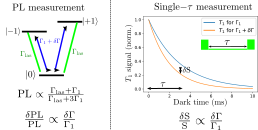
\includegraphics[width=0.9\textwidth]{chapter 2/Figures/relaxo_pulsed_continuous}
\caption{Representation of the two relaxometry protocol. Left : representation of the three level system of the NV center with the polarization rate $\Gamma_{\rm las}$ and spin decay rates $\Gamma_1=1/T_1$ and the perturbation $\delta \Gamma$. Right: simulation of a $T_1$ measurement for $1/\Gamma_1=3\ \rm ms$ and $1/(\Gamma_1+\delta \Gamma)=2\ \rm ms$. $\delta \rm S$ represents the maximum difference in signal between the two curves for a dark time $\tau$.}
\label{T1 vs PL}
\end{figure}

There are two ways to measure a change in the spin $T_1$, as represented on Fig. \ref{T1 vs PL}. The first and most basic method simply consist in monitoring the PL of the NV centers : since the PL is proportional to the population in the $\ket{0}$ state, which itself results from an equilibrium between the polarization rate $\Gamma_{\rm las}$ and the spin decay rate $\Gamma_1=1/T_1$. A change in $\Gamma_1$ will therefore conduct to a new equilibrium with a different PL. 

The second method is a pulsed sequence referred as single$-\tau$ measurement, used for example in \citep{pelliccione2014two, schmid2015relaxometry, tetienne2016scanning}. It simply consists in a $T_1$ measurement sequence (as seen in chapter 1) where you first polarize the spins in the $\ket{0}$ state with a laser pulse and read out the spin state with a second laser pulse after a dark time $\tau$. In this case however, instead of scanning the time $\tau$, you fix its value to maximize the sensitivity in a change of $T_1$ (typically $\tau \approx T_1$). 

It is argued in \citep{finco2021imaging} that both methods result in similar signal to noise ratio: in the first case you need to adjust $\Gamma_{\rm las} \sim \Gamma_1$ to maximize the PL contrast, meaning that the laser power used is very far from the saturation limit (typically $\Gamma_1 \approx 10^3\ \rm s^{-1}$ and $\Gamma_{\rm sat} = 5\cdot10^6\ \rm s^{-1}$\citep{dreau2011avoiding}), while the second method needs to wait a time $\tau \sim T_1$ between each measurement, which result in a similar PL count and shot noise limit in both case.

On a technical level, the PL-based method is easier to implement since it does not require the use of a pulsed laser, and uses an overall smaller laser power, however it is more sensitive to drifts and changes in the optical setup. Most of the relaxometry measurement in this manuscript were performed using a PL-based detection.

\subsection{Comparison with DEER protocol}

\begin{figure}[h]
\centering
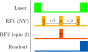
\includegraphics[width=0.5\textwidth]{chapter 2/Figures/DEER}
\caption{Pulse sequence of the DEER protocol}
\label{DEER}
\end{figure}

Outside of cross-relaxations, another protocol exists to address dark spin resonance with NV centers, based on a modification of the NV $T_2$ time \citep{serbyn2014interferometric}. This protocol called double electron-electron resonance (DEER) is depicted on Fig. \ref{DEER}. The pulse sequence consist in a spin-echo sequence on the NV center, as described in chapter 1, with a simultaneous $\pi-$pulse on the probed dark spins during the rephasing pulse on the NV centers. This additional pulse means that the static (or slowly variable) contribution of the probed spins to the $T_2^*$ of the NV center wont be rephased. The newly measured $T_2$ time should therefore be slightly shorter:

\begin{equation}
\frac{1}{T_2^{\rm DEER}}=\frac{1}{T_2^{\rm echo}} + \delta \Gamma_2^*,
\end{equation}

where $\delta \Gamma_2^*$ is the contribution of the dark spin to the $T_2^*$ of the NV center.

By scanning the frequency of the second microwave (RF2) and monitoring the $T_2$ time of the NV centers, one can therefore find dark spin resonance without having to bring them to resonance with NV centers, which can be useful when the dark spin resonance is very far detuned from the NV one.

While both cross-relaxation and DEER measure the dipole-dipole coupling of dark spins to an NV center, there are several differences between the two protocols:

Frist, the two protocols do not measure the same elements of the dipole-dipole Hamiltonian: CR measures the off-diagonal elements $\Omega_{\rm CR}=\mel{i,j}{\mathcal{H}_{\rm dd}}{j,i}/\hbar$ which are responsible for the flip-flops or double flips, while DEER measures the diagonal elements $\Omega_{\rm DEER}=\mel{i,j}{\mathcal{H}_{\rm dd}}{i,j}/\hbar$ which are responsible for the pure dephasing. These terms however are on average of the same amplitude, and when averaging over an ensemble we can consider $\Omega_{\rm CR} \sim \Omega_{\rm DEER}$

Second and more importantly, the scaling is not the same in both cases : CR measures a change in the NV decay rate $\Gamma_1=1/T_1$ which is proportional to $\Omega_{\rm CR}^2$, as given by eq. \ref{delta gamma 1}, while DEER measures a change in $\Gamma_2=1/T_2$ which is proportional to $\Omega_{\rm DEER}$, as given by eq. \ref{Gamma2 P1}. This means that the signal of CR scales quadratically with the impurity concentration, while the DEER signal scales linearly with it. CR is therefore more suited to probe concentrated impurities, when the average distance between the NV and the probed spin is small.

\section{Choice of the magnetic field orientation}

Since relaxometry does not rely on a microwave field, the only parameter left to tune is the external magnetic field, which is often scanned with an electromagnet. Due to the strong NV anisotropy however, the direction along which $\mathbf{B}$ is scanned plays a crucial role in the ability to detect dark spins.

\subsection{The [100] and [111] magnetic field orientations}
\label{sec simu}

\begin{figure}[h]
\centering
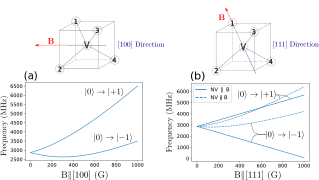
\includegraphics[width=0.9\textwidth]{chapter 2/Figures/121_vs_22_NV}
\caption{Simulated transition frequencies of the $\ket{0} \to {-1}$ and $\ket{0} \to {+1}$ transitions for the 4 classes of NV centers as a function of the magnetic field. a) When the magnetic field is along the diamond [100] crystalline axis, b) along the [111] axis. A representation of the 4 classes of NV centers, labeled 1 to 4, and the orientation of the magnetic field in both cases is put on top}
\label{121 vs 22 NV}
\end{figure}

Fig. \ref{121 vs 22 NV} shows the two main choices of scanning orientation : either $\mathbf{B} \parallel [100]$ or 
$\mathbf{B} \parallel [111]$ where [100] and [111] refer to the diamond crystalline axes as defined in chapter 1. When $\mathbf{B} \parallel [100]$, all four classes (the different possible NV orientations represented at the top of the figure) are equivalent, whereas for $\mathbf{B} \parallel [111]$, one class is perfectly aligned with the magnetic field while the three others are equivalently unaligned. 

These changes in the field orientation result in massive changes in the NV behavior, manly due to the transverse magnetic field: Fig. \ref{121 vs 22 NV}-a) shows the transition frequency between the $\ket{0}$ and $\ket{\pm 1}$ states of the ground state spin Hamiltonian (REF chapter 1) - or to be more precise the transitions between the ground state of the spin Hamiltonian and the two excited states - for any of the four classes of NV centers when $\mathbf{B} \parallel [100]$. Notably, there is no transitions frequencies below 2500 MHz. 

On the other hand, Fig. \ref{121 vs 22 NV}-b) shows the transition frequencies when $\mathbf{B} \parallel [111]$, for both the class aligned and the three class misaligned. The three classes behave similarly than the four classes in the $[100]$ case, but the one class aligned with the magnetic field can get its $\ket{0}\to\ket{-1}$ transition arbitrarily small, as long as the magnetic field is perfectly aligned with the NV axis.

\subsection{CR condition between NV$^-$ and P1}

\begin{figure}[h]
\centering
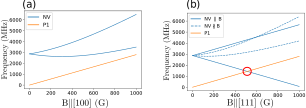
\includegraphics[width=0.9\textwidth]{chapter 2/Figures/121_vs_22_P1}
\caption{Simulation of the transition frequencies of NV$^-$ centers and P1 centers (without the hyperfine interactions) for a magnetic field a) along the [100] axis and b) along the [111] axis}
\label{121 vs 22 P1}
\end{figure}

P1 centers, the most abundant electronic spin in the diamonds commonly used, have a $1/2$ electronic spin. They do have a small magnetic field anisotropy coming from the hyper-fine coupling to the nitrogen nucleus ($\sim 100\ \rm MHz$), but this dependency on the field orientation is small compared to the NV center's zero field splitting $D=2870\ \rm MHz$. We can therefore, to the first order, neglect the hyper-fine coupling and consider P1 centers as ideal, isotropic, spin $1/2$.

Fig. \ref{121 vs 22 P1} shows the transition frequencies for the NV center and such a spin $1/2$, as a function of a magnetic field parallel to [100] or [111]. When $\mathbf{B} \parallel [100]$, there will never be a co-resonance between the NV and P1 transitions, meaning that no NV-P1 cross-relaxation can be observed when B is scanned in this direction. When $\mathbf{B} \parallel [111]$ however, the P1 $\ket{-1/2} \to \ket{+1/2}$ transition matches in energy the $\ket{0}\to\ket{-1}$ NV transition for B=512 G. This means that when B reaches $\approx 512\ \rm G$, some of the polarization of the NV centers will be transferred to the P1 centers, which will result in a drop in the NV PL. 

\subsection{CR condition between NV$^-$ and VH$^-$}

\begin{figure}[h]
\centering
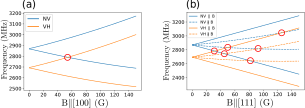
\includegraphics[width=0.9\textwidth]{chapter 2/Figures/121_vs_22_VH}
\caption{Simulation of the transition frequencies of NV$^-$ centers and VH$^-$ centers for a magnetic field a) along the [100] axis and b) along the [111] axis}
\label{121 vs 22 VH}
\end{figure}

VH$^-$, a much less abundant electronic spin than P1 center, has an electronic spin 1, with a spin Hamiltoninan very similar to that of the NV center. In particular it has the same symmetries being also a $C_{3v}$ defect, with a slightly smaller ZFS at $D_{VH} \approx 2700\ \rm MHz$ compared to $D_{NV}=2870\ \rm MHz$. 

Fig. \ref{121 vs 22 VH} shows the transition frequencies for the NV$^-$ and VH$^-$ ground state spin. Contrary to the P1 case, there is a co-resonance when $\mathbf{B} \parallel [100]$ for $B\approx 55\ \rm G$. When $\mathbf{B} \parallel [111]$, there are 6 co-resonance conditions between 30 and 130 G. A scan along the [111] in this case means that the peak signal will be $\sim 6$ times weaker than in the [100] case, and spread over multiple lines which might overlap between themselves or with other existing PL features.

The War1 spin mentioned previously is also an electronic spin 1 with (pseudo)-$C_{3v}$ symmetry and $D_{War1} \approx 2470\ \rm MHz$. This result in a similar behavior than VH$^-$ when it comes to the CR condition with NV centers.

\subsection{CR condition between NV$^-$ and and $^{13}$C-NV$^-$}

\begin{figure}[h]
\centering
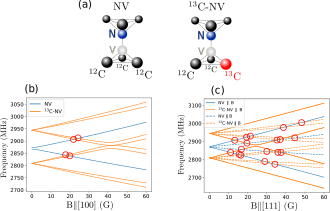
\includegraphics[width=1\textwidth]{chapter 2/Figures/121_vs_22_13CNV}
\caption{a) Representation of the $^{13}$C-NV complex (right) compared to a ``normal" NV center (left) b) and c) simulation of the transition frequencies of NV$^-$ centers and $^{13}$C-NV$^-$ complex for a magnetic field b) along the [100] axis and c) along the [111] axis}
\label{121 vs 22 13C-NV}
\end{figure}

I refer by $^{13}$C-NV$^-$ to a complex formed by an NV center where one of the three carbon atoms neighboring the vacancy is a $^{13}$C isotope. Such a complex is illustrated in Fig. \ref{121 vs 22 13C-NV}-a).

The $^{13}$C-NV$^-$ complex still behaves as a ``normal" NV center, except that its transition lines are shifted by the hyper-fin coupling. In particular its electronic spin is still polarized in the $\ket{0}$ state and the $\ket{0}$ state is still brighter than the $\ket{\pm 1}$ states. This is confirmed by the presence of sideband in ODMR spectra around the main NV lines \citep{simanovskaia2013sidebands}.

Since both NV$^-$ and $^{13}$C-NV$^-$ are \textit{a priori} equally polarized, then following the argument in \ref{Sec_CR} there should be no CR between the two spin families. The reason why those transitions are still in some case visible, as will be shown below, and why in fact any NV-NV co-resonance gives a visible CR signal will be the object of the next chapter.

The transitions of the $^{13}$C-NV$^-$ complex are given by diagonalizing the full spin Hamiltonian:
\begin{equation*}
\mathcal{H}=\mathcal{H}_{NV}+\mathcal{H}_{^{13}C}+\mathcal{H}_{HF},
\end{equation*}
where $\mathcal{H}_{NV}$ is the NV$^-$ spin Hamiltonian,
$\mathcal{H}_{^{13}C}$ is the $^{13}$C nuclear spin Hamiltonian for a $1/2$ spin : $\mathcal{H}_{^{13}C}=\gamma_{n} B I_z$ where $\gamma_{n}=$10.7 MHz/T is the $^{13}$C gyromagnetic ratio, and $\mathcal{H}_{HF}$ is the hyper-fine interaction Hamiltonian: $$\mathcal{H}_{HF}= \hat{\mathbf{S}}_{NV} \cdot \mathcal{A} \cdot \hat{\mathbf{I}}_C.$$

When the $^{13}$C is the direct neighbor of the vacancy as represented in Fig. \ref{121 vs 22 13C-NV}-a) - this is also referred as a first-shell $^{13}$C - the hyper-fine tensor $\mathcal{A}$ can be written \citep{simanovskaia2013sidebands}:
$$ \mathcal{A} = \begin{pmatrix}
\mathcal{A}_{xx} & 0 & \mathcal{A}_{xz} \\ 0 & \mathcal{A}_{yy} & 0 \\ \mathcal{A}_{zx} & 0 & \mathcal{A}_{zz}
\end{pmatrix},$$
where $\mathcal{A}_{xx}=190$ MHz, $\mathcal{A}_{yy}=120$ MHz, $\mathcal{A}_{zz}=129$ MHz, and  $\mathcal{A}_{xz}=\mathcal{A}_{zx}=-25.0$ MHz. 

Fig. \ref{121 vs 22 13C-NV}-b) and c) show the simulated transition frequencies for a $^{13}$C-NV$^-$ complex when B is scanned along the [100] or [111] axis, as well as the ``normal" NV transitions and the co-resonance between those two. When $\mathbf{B} \parallel [100]$, there are 4 co-resonances between 18 and 25 G. When $\mathbf{B} \parallel [100]$ there are 18 of them between 10 and 60 G. This abundance of transitions for low ($<100\ \rm G$) magnetic field makes analyzing experimental data quickly intractable in the second case.

\subsection{CR contrast and transverse magnetic field}
\label{CR contrast}

\begin{figure}[h]
\centering
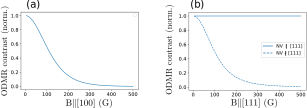
\includegraphics[width=0.9\textwidth]{chapter 2/Figures/contrast_OMDR_111_Vs_100}
\caption{Simulated ODMR contrast on all four classes of NV centers with a magnetic field a) along the [100] axis and b) along the [111] axis}
\label{121 vs 22 contrast}
\end{figure}

In order to optically detect CR between an NV center and a dark spin, two conditions must be met: the NV center must be polarized in order to have a population transfer between the NV and the dark spin, and there must be a difference in brightness between the two NV levels involved in order to have an optical signature of the CR.

These two conditions are in fact the same needed to observe an ODMR spectrum (REF chapter 1), and while the NV centers verifies both criteria in presence of a purely longitudinal magnetic field, this is not always the case anymore in presence of a transverse magnetic field (REF chapter 1).

Fig. \ref{121 vs 22 contrast} shows the simulated relative contrast of an ODMR spectrum, as computed from \citep{tetienne2012magnetic}, for a magnetic field aligned along [100] or [111]. When the NV center is aligned with the magnetic field, the constrats remains equals to 1 regardless of the magnetic field because there is no transverse field. When the NV is not aligned however, either in the [111] or [100] case, the ODMR contrast quickly drops down for B$>100\ \rm G$.

This tells us that we should not expect to observe a CR signal for B greater than a few hundreds G when B is scanned along the [100] axis. We could however observe CR for arbitrarily large magnetic field when scanned along the [111] axis, as long as the field is properly aligned with the NV axis.

\section{Dark spin spectroscopy with NV centers}

\subsection{Detection of P1 centers}

\begin{figure}[h]
\centering
\includegraphics[width=0.7\textwidth]{chapter 2/Figures/NV_P1_libreAcces}
\caption{Change in the PL of an ensemble of NV centers as a magnetic field is scanned along the [111] crystalline axis. Taken from \citep{armstrong2010nv}}
\label{CR P1 exp}
\end{figure}

Previously to our work, several studies \citep{van1989cross, holliday1989optical, epstein2005anisotropic, armstrong2010nv,   hall2016detection, wickenbrock2016microwave,  wood2016wide,  alfasi2019detection, lazda2021cross} had been done on the detection of dark spins through CR with NV centers, and to our knowledge, all this studies where done on the detection of P1 centers. Following the discussion in the last section, these studies were therefore all done with $\mathbf{B} \parallel [111]$.

An example of one of this study (\citep{armstrong2010nv}) is shown in Fig. \ref{CR P1 exp}. It shows the evolution of the NV PL with respect to a magnetic field scanned along the [111] crystalline axis. There are several information to gather from this graph:

First, there is the slowly decaying PL envelope, which stabilizes to a plateau for $B\sim 1000\ \rm G$. This change in PL is caused by the transverse magnetic field acting on the three NV classes that are not aligned with the magnetic field. For $B \gtrsim 1000\ \rm G$, these three classes are fully depolarized which explains the plateau observed.

Second, there are the three salient features denoted Ns-NV, NV-NV and NV-LAC. All these features come from cross-relaxations or level anti-crossing (LAC) from the NV class aligned with the magnetic field.

The first feature (Ns-NV) for $B\approx 512 \ \rm G$ is the signature of the CR between NV and P1 centers. Its relatively complicated shape comes from the hyper-fine coupling between the P1 electronic spin and the $^{14}$N nucleus \citep{lazda2021cross}. Excited state level anti-crossing (ESLAC) also occurs in this region, but its optical signature, if it exists, is expected to be much weaker than the NV-P1 CR \citep{zheng2017level}.

The second feature (NV-NV) for $B\approx 590 \ \rm G$ comes from the cross relaxation between NV centers aligned with the magnetic field and NV centers misaligned with the field (the co-resonance can be observed in Fig. \ref{121 vs 22 NV}-b)). This phenomenon will be further discussed in the next chapter.

Finally the third feature (LAC) for $B\approx 1024 \ \rm G$ correspond to the level anti-crossing between the $\ket{0}$ and $\ket{-1}$ states of the NV center aligned with B. When the two levels get close enough in energy, the Hamiltonian off-diagonal terms (coming from strain local electric field or residual transverse magnetic field) will mix the $\ket{0}$ and $\ket{-1}$ states and prevent an efficient polarization by the green laser. This result in a sharp drop in the PL that can be exploited to perform microwave-less magnetometry with NV centers \citep{wickenbrock2016microwave, zheng2017level, zheng2020microwave}.

\subsection{Detection of VH$^-$, War1 and $^{13}$C-NV$^-$}

\begin{figure}[h]
\centering
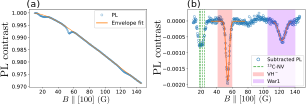
\includegraphics[width=\textwidth]{chapter 2/Figures/fig_VH_et_co}
\caption{a) Change in PL (normalized) of the ensemble of NV centers in sample CVD-pink as a magnetic field is scanned along the [100] axis. The orange line is a fit to the slowly decreasing envelope b) Subtraction of the PL signal by the envelope fit as a function of the magnetic field. The green lines and red and purple regions correspond to the predicted CR regions, as detailed in main text}
\label{CR VH exp}
\end{figure}

Our work \citep{pellet2021optical} focuses on the optical detection of VH$^-$, War1 and $^{13}$C-NV$^-$ through NV CR. This study was the first to detect VH$^-$ and War1 defects optically and the first CR experiment on a CVD diamond. It was also the first,to our knowledge, to use a [100] aligned magnetic field.

The diamond used for this study is the sample CVD-pink [REF appendix] whose fabrication was detailed in \citep{tallaire2020high}. It is a CVD diamond containing $[\rm NV ]\approx 4\ \rm ppm$ for $[\rm N ]\approx26\ \rm ppm$, and a natural abundance (1.1\%) of  $^{13}$C. Being a CVD diamond it is also likely to incorporate hydrogen defects, as discussed in \ref{other defects}.

Fig. \ref{CR VH exp}-a) shows the change in PL with respect to a magnetic field scanned along the diamond [100] axis. Similarly to fig. \ref{CR P1 exp}, we can see a slowly decaying envelope of the PL due to the transverse magnetic field (we don't see the plateau here since the magnetic field stops at 150 G). We can also see three deviations to the smooth decreasing curve at $\sim$ 20 G, 55 G and 120 G.

In order to better discern the three features, we fitted the envelope by using a polynomial fit of order 4 on the smooth part of the data. We previously tried to use a fit based on the expected PL rate of the NV centers, by using the model in \citep{tetienne2012magnetic}, but the results were not satisfying.

Fig. \ref{CR VH exp}-b) shows the subtraction of the PL data by the envelope fit. We can clearly see three dips in PL around the values 20 G, 56 G and 122 G. We then computed the expected value of the magnetic field for the expected CR line thanks to the simulations shown in sec. \ref{sec simu}. For the VH$^-$ and War1 lines, we took the ZFS $D$ values from \citep{cruddace2007magnetic} and included the error bars. For the $^{13}$C-NV$^-$ lines, the error bars given in \citep{simanovskaia2013sidebands} are much smaller and we only plotted the expected value. We can see that the dips in PL match relatively well the predicted CR lines of $^{13}$C-NV$^-$, VH$^-$ and War1 respectively.

The experimental setup used to obtain this data is the standard confocal microscopy setup shown in appendix REF. The magnetic field here is generated with an electromagnet (EM), aligned along the [100] diamond axis with a precision $<1^\circ$. 

The data shown here was acquired over 24 h. It should be noted however that a single-photon counting APD was used here, which considerably worsens the sensitivity of the measurement as discussed in [REF]. Using a photodiode and modulation of the magnetic field, we estimate that we could get similar signal to noise ratio within a few minutes.

To calibrate the magnetic field, we added a microwave field at a  fixed frequency $\nu > 2870\ \rm MHz$, and measured the EM voltage at which the PL dropped due to the $\ket{+1}$ state of the NV centers becoming resonant with the microwave tone. We could then use the values in Fig. \ref{121 vs 22 NV} to find the corresponding magnetic field. We varied the frequency in the range  $[2870,3150]\ \rm MHz$ by step of 2 MHz to get a calibration of the magnetic field in the $[0,150]\ \rm G$ region. Considering the uncertainty in the field angle, the NV ZFS $D$ value and the width of the PL drop, we estimate the final precision of the calibration to be within $\pm 1\ \rm G$.

\section{Attribution of the $^{13}$C-NV$^-$, VH$^-$ and War1 lines}

\subsection{The VH$^-$ and War1 lines}
\begin{table}[htbp]
\centering
\caption{\bf Zero-field splitting parameter $D$ for NV$^-$, VH$^-$ and War1}
\begin{tabular}{ccc}
\hline
$D_z$ estimation (MHz) & Cruddace's work\citep{cruddace2007magnetic} & Our work \\
\hline
NV$^-$ & 2872(7) & * \\
VH$^-$ & 2706(30) & 2694(5)  \\
WAR1 & 2466(60) & 2470(10) \\
\hline
\end{tabular}
  \label{table VH et War1}
\end{table}

The attribution of the PL dips at 56 and 122 G in Fig. \ref{CR VH exp} to CR between NV and respectively VH$^-$ and War1 comes from two main observations: the closeness in the ZFS values, and the CVD nature of the sample.

Table \ref{table VH et War1} shows the value and precision of the $D$ factor when measured through EPR \citep{cruddace2007magnetic}, and when computed from the data in Fig. \ref{CR VH exp}. In order to get to the $D$ value of VH$^-$ and War1, we had to assume that the spin structure was that of a spin 1 similar to the NV center, with a g-factor close to 2. Both of this assumptions are confirmed by the EPR measurements. We do find that that both $D$ measurement concord within their respective error bars.

The second reason comes from the nature of the sample used. We tried similar PL scans along the [100] axis on many samples with dense ensemble of NV centers. We found that the dip at 55 G was present on all CVD samples ($\sim$ 5 samples) used, and none of the HPHT samples ($\sim$ 20 samples). The same is true of the 122 G line, except that it did appear on some HPHT samples, as will be discussed below. We know that the VH$^-$ defect is much more likely to appear in a CVD sample due to the large quantity of hydrogen used in the process, and while we don't know the chemical nature of the War1 defect, the only time it was observed through EPR was on a CVD diamond.

Finally, the apparent larger linewidth of the War1 line compared to the VH$^-$ one is also corroborated by the EPR measurements.

For all of this reasons we attribute the 55 and 122 G dip to CR with VH$^-$ and War1 respectively, with a slightly stronger confidence for the VH$^-$ since more is known about it.

\subsection{The $^{13}$C-NV$^-$ lines}

\begin{figure}[h]
\centering
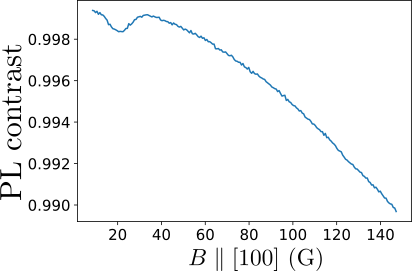
\includegraphics[width=.6\textwidth]{chapter 2/Figures/scan_100_Sumi4}
\caption{Change in PL as a function of a magnetic field scanned along the [100] axis for sample SUMI-4}
\label{scan sumi 4}
\end{figure}

The attribution of the $\sim 20\ \rm G$ dip to CR with $^{13}$C-NV$^-$ also come from two observations. First, the lines are present on every single sample with dense ensemble ($\gtrapprox 1$ ppm), regardless of the fabrication process. Fig. \ref{scan sumi 4} for example shows a PL scan along the [100] axis for sample Sumi-4, an HPHT sample with [NV]$\approx 5\ \rm ppm$ and natural abundance of $^{13}$C. I could unfortunately not try a sample isotopically enriched in $^{12}$C since those samples are generally reserved to low-nitrogen concentration ($< 10\ \rm ppm$), which does not yield enough NV centers to perform CR spectroscopy. 

The second reason is the shape of the PL dip. The two other dips seem be formed of a single line and are reasonably well fitted with Gaussian curves. The 20 G dip however has a flat bottom which would indicate the presence of several overlapping lines, and Fig. \ref{121 vs 22 13C-NV} indeed predicts that there would be 4 CR lines between 18 and 25 G.

For this two reasons, we attribute the 20 G line to CR between $^{13}$C-NV$^-$ and ``normal" NV centers.

\section{Quantitative estimates of the NV-Dark spins CR}

We can extract some quantitative information about the dark spins by exploiting the CR spectrum shown in Fig. \ref{CR VH exp}.

\subsection{Dark spin Hamiltonian parameters}

First, as discussed in the last section, we can estimate the dark spin ZFS $D$ value with greater precision than EPR. While it would be in theory possible to measure other properties of the dark spins Hamiltonian - such as the $g$-factor - by changing the angle of the magnetic field, this would here quickly become intractable due to the increase in co-resonance conditions and the relative closeness of each of these transitions. DEER might prove more useful in this regard as only one class of NV centers at a time is probed.

\subsection{Dark spin linewidth}

The second quantitative estimate we can make is of the dark spin inhomogeneous broadening $T_2^*$: if we assume the change in PL to be proportional to the change in the NV lifetime $T_1$, which is true for small enough changes, then the linewidth of the PL dips in Fig. \ref{CR VH exp} is the convolution of the NV and dark spin spectrum. By deconvoluting the data with the NV spectrum, known for example from ODMR, we can then recover the dark spin spectral response as was done in \citep{hall2016detection}. 

This procedure will be discussed in more details in the next chapter. We find here that the linewidth of VH$^-$ and War1 are respectively [REF] and [REF] MHz.

\subsection{Dark spin concentration}

Finally, the third tentative estimate we can make is that of the dark spins concentration. We can indeed calibrate the measurement by using the $^{13}$C-NV$^-$ line, of which we know the concentration in natural abundance diamond: [$^{13}$C-NV$^-$] $\approx$ 3.3 \% [NV]. We can then, knowing the NV concentration, try to estimate the concentration of the dark spins. There are several caveats though:

\begin{itemize}
\item Since the change in $T_1$ is proportional to the $T_2^*$ of the probed spins (eq. \ref{delta gamma 1}), we should compensate that by integrating over the entire feature, instead of simply looking at the maximum of the line.
\item We have to take into account the loss of contrast of the NV centers as the transverse magnetic field grows, as explained in sec. \ref{CR contrast}.
\item The $^{13}$C-NV$^-$ are not ``dark spins", and its CR feature cannot be \textit{a priori} compared to the one from VH$^-$ and War1. We will see however in the next chapter that we can consider a fraction of the NV centers as dark spins, and that this fraction can be estimated. \citep{choi2017depolarization} found a ratio of $\sim 1/4$ dark NV centers for $\sim 3/4$ bright ones.
\end{itemize}

With all this considerations, we can give an estimate of the concentrations of VH$^-$ and War1 based on the data on Fig. \ref{121 vs 22 VH}-b): 

For the VH$^-$ line we find that the area of the line is $\approx 1.4$ times bigger than that of the $^{13}$C-NV$^-$ one, from \ref{121 vs 22 contrast} we find that the expected CR contrast is $\approx 1.2$ times smaller at 55 G than at 20 G, and finally we chose the dark to bright NV ratio value from \citep{choi2017depolarization} at 0.25.

With an estimated NV concentration [NV] $\approx\ \rm 4.6 ppm$, giving us a concentration $[^{13}\rm{C-NV}^-]\approx \ \rm 130 ppb$, we then find $[\rm VH^-] \approx 58\ \rm ppb$. Similarly, we find $[\rm VH^-] \approx 68\ \rm ppb$. Given the large uncertainty on some parameters, in particular the dark to bright spin ratio, these estimates are probably only precise within an order of magnitude.

If we consider that the sampled volume in this experiment is $< 100 \mu \rm{m}^3$, the total number of dark spins detected here is then $< 10^6$. Even with very conservative estimates, the technique employed here is still more sensitive than EPR by several orders of magnitude.

\section{Temperature dependence of VH$^-$ and War1}


\subsection{Mofifications on CVD samples}
\begin{figure}[h]
\centering
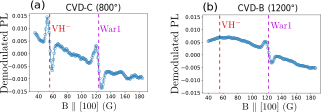
\includegraphics[width=\textwidth]{chapter 2/Figures/VH_CVD_chauffage}
\caption{Demodulated PL on samples CVD-C and CVD-B as a function of a magnetic field along the [100] axis. An additional oscillating magnetic field along the same direction was used to perform the lock-in detection. The VH$^-$ and War1 lines are taken from \ref{CR VH exp}}
\label{chauffage CVD}
\end{figure}

Given that the NV CR spectroscopy was both sensitive and relatively easy to setup, we decided in collaboration with the teams of Alexandre Tallaire at IRCP and Jocelyn Achard at LSPM to study the effect of annealing at high temperature on VH$^-$ and War1 \citep{ngambou2022improving}.

Fig. \ref{chauffage CVD} shows the results of this experiment. This time, a modulation of the magnetic field was used and the PL coming from the photodiode was demodulated through a lock-in amplifier, which explains the derivative shape of the lines. The fact that the background is not perfectly flat still comes from the transverse magnetic field. The same lock-in parameter were used on both plots so that the amplitudes should in theory be comparable.

Fig \ref{chauffage CVD}-a) shows the demodulated PL versus mganetic field amplitude along [100] on sample CVD-C, while \ref{chauffage CVD}-b) shows the same experiment on sample CVD-B. The fabrication and subsequent operations done on this two samples are detailed thoroughly in \citep{ngambou2022improving}, but the main difference between these two sample is that CVD-C was only annealed once after irradiation, for 2 hours at 800$^\circ$C, while CVD-B was annealed for 2 hours at 800$^\circ$C and then for 1 hour at 1000$^\circ$C and 1 hour at 1200$^\circ$C.

We can see that the VH$^-$ line in particular completely disappear on sample CVD-B, which we attribute to the additional annealing. This measurement also corroborate modifications in the infrared absorption spectrum, and an increase of the NV coherence time, associated with the annealing at higher temperature \citep{ngambou2022improving}.

The War1 line on the other hand is still present after the high temperature annealings, albeit slightly smaller. This information can give us some insights on the chemistry of the War1 defect. %Et en vrai je crois que c'était deja vu dans la thèse de Cruddace

\subsection{Modification on HPHT samples}

\begin{figure}[h]
\centering
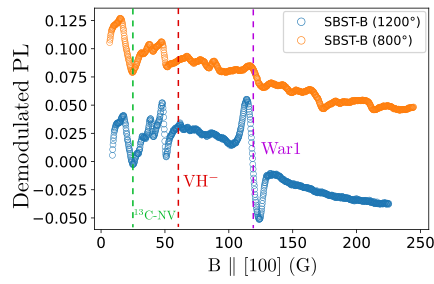
\includegraphics[width=.7\textwidth]{chapter 2/Figures/VH_HPHT_chauffage}
\caption{Demodulated PL on samples SBST-C and SBST-B as a function of a magnetic field along the [100] axis. The plot of SBST-C is offset for clarity}
\label{chauffage HPHT}
\end{figure}

An unexpected side-study was done on HPHT samples. Indeed, the CVD samples used previously are grown by homoepithaxy on top of a diamond substrate. In this case, the substrate was a type 1B HPHT diamond, which was irradiated and annealed along the CVD layer. We Will name SBST-C and SBST-B the respective HPHT substrate of CVD-C and CVD-B.

Fig. \ref{chauffage HPHT} shows demodulated PL scans with B $\parallel$ [100] on both samples. They both show a line at $B \approx 20\ \rm G$ corresponding to the $^{13}$C-NV$^-$ line, and none of them show a line at $B = 56\ \rm G$ corresponding to the VH$^-$ line. There is however a stark difference for the War1 line: SBST-C seems to show a weak line, while SBST-B shows a very clear line, with an amplitude more than 5 times greater than SBST-C. 

We can also see that many weak lines on SBST-B seems to have disappeared in SBST-C, while an unidentified line at $B = 48\ \rm G$ seems to have grown similarly to the War1 line.

We first suspected that some of the War1 defects had been migrating from the CVD layer to the HPHT substrate with the high-temperature annealing, but not only is it very unlikely with the annealing time (1 hour) and substrate thickness (several mm), We also could not find a dependence on the War1 concentration with the depth in the substrate, whereas a diffusion would have given a higher concentration near the CVD layer. The War1 defects seem to have been created by the annealing.

These results suggest that, while some defects are removed by the high temperature annealing, such as the VH$^-$ and several unidentified defects in the HPHT substrate, some seem to be created by the annealing process, such as the War1 or the one associated with the line at $B = 48\ \rm G$ in the HPHT substrate.

\section{Conclusion and perspectives}

To conclude this chapter, we have seen how NV centers can be used to detect dark spins via cross-relaxations. This detection can be way more sensitive than the usual EPR spectroscopy, and considerably cheaper to set up. It is however not as versatile and should be seen as a complimentary tool for diamonds with dense NV ensemble. 

We have also seen the importance of the magnetic field direction, and the underused aspect of the [100] magnetic field scan, much less noisy than the [111] scans for weak magnetic field.

Finally we have seen an application of the CR to detect optically two dark spins in CVD diamond, and to find out the response of these defects to high temperature annealing.

There still remains a lot of open questions and there are several experiments that could be build upon these results. I will list some of them here.

\subsection{Unidentified CR lines}

There are still a large number of lines in CR spectra that have not been identified. While not every line necessarily correspond to a new defect - for example \citep{wunderlich2021magnetic} recently found lines corresponding to co-resonance between the $\ket{0} \to \ket{-1}$ transition of an NV center and the $\ket{-1} \to \ket{+1}$ of another NV center - the more likely hypothesis for each of these unidentified lines is still the presence of a new defect.

Such unidentified lines can be seen in Fig. \ref{chauffage CVD} and \ref{chauffage HPHT}. In particular we can see a line at 160 G in Fig. \ref{chauffage CVD}-a) and a line at 48 G in Fig. \ref{chauffage HPHT} that detach clearly from the background. 

Further studies would be needed to find how common these lines are, and what could be there sources.

\subsection{Measuring the spin dynamics of VH$^-$}

We found that NV-VH$^-$ CR in CVD could produce a change in PL of $\sim 0.2 \%$. This kind of values are not too far from ODMR contrast with NV ensembles, which means that it would be reasonable to probe the dynamics ($T_1$, $T_2$) of the VH$^-$ spin. The main issue comes from the fact that in order to measure the VH$^-$ spin states, it needs to be resonant with the NV center. Therefore, resonant microwave pulses with VH$^-$ will also be resonant with the NV centers, which will create an unwanted optical signal.

There are two solution to circumvent this problem: the first is to use a fast switching magnetic field in order to bring the VH$^-$ and NV centers in resonance when you want to polarize or readout the VH$^-$ state, and out of resonance when you want to coherently manipulate the VH$^-$. This means that the magnetic field needs to be switched faster than the spin dynamics you want to probe. This might be doable for the population dynamics $T_1$ but this is probably too slow to probe the $T_2$ time.

The other solution consists in using the spin-1 nature of VH$^-$: when a NV$^-$-VH$^-$ CR occurs, only one of the transitions of VH$^-$ and NV$^-$ is brought to resonance. The other one ($\ket{0} \to \ket{-1}$ for the VH$^-$) is out of resonance. The idea would therefore be to keep the NV $\ket{0} \to \ket{-1}$ transition and VH $\ket{0} \to \ket{+1}$ transition resonant, and to coherently manipulate the VH $\ket{0} \to \ket{-1}$ transition. While the polarization on this transition, and the back-action it would produce on the NV centers, is not as strong as if you were manipulating the $\ket{0} \to \ket{+1}$ transition, it should still produce a measurable signal.

\subsection{Isolating a single VH$^-$}

We estimated the concentration of VH$^-$ in CVD-pink to be $\sim 60\ \rm ppb$. This concentration is too high by about two orders of magnitude to isolate a single emitter with a diffraction-limited microscope. We know however that we can reduce the VH$^-$ concentration arbitrarily by applying high temperature annealing. We could therefore reduce the VH$^-$ concentration to be in the $0.1 \sim 1\ \rm ppb$ range and optically isolate a single VH$^-$ center by scanning a confocal microscope with a fixed $B_{[100]}=56\ \rm G$ while monitoring the NV PL or $T_1$. It is however unclear to me whether this detection scheme would be sensitive enough to detect single dark spins.

\printbibliography
\end{refsection}
 \begin{refsection}

\chapter{NV-NV cross-relaxations : the fluctuator model}
In this chapter we will look at the phenomenon of cross-relaxations between NV centers, both from an experimental and theoretical point of view. 

The presence of strong NV-NV dipolar interaction in dense ensemble ([NV] $\gtrsim 1\ \rm ppm$) proved to be both an obstacle for ensemble magnetometry \citep{zhou2020quantum} and an opportunity to explore and use the many-body interaction resulting from it \citep{zhou2020quantum, choi2017observation, kucsko2018critical, zu2021emergent}.

We will see here how a model of fast and slow relaxing centers, the fluctuator model \citep{choi2017depolarization}, can explain most of the experimental observations, and we will see some limitations of the model.

\section{Experimental observation of NV-NV CR}
Before we discuss the theoretical implications of NV-NV cross-relaxations (CR), let us first show the unambiguous experimental proof of the presence of NV-NV CR in the samples with dense NV ensembles.
\subsection{NV-NV CR between nonequivalent NV centers}
\label{non_equi_valent_CR}
\begin{figure}[h]
\centering
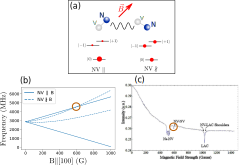
\includegraphics[width=\textwidth]{chapter 3/Figures/NV-NV_non_equivalent}
\caption{a) Representation of two non equivalent spins resonantly coupled. One spin is aligned with the magnetic field and therefore well polarized, while the second spin is not. b) Simulated frequencies for the $\ket{0} \to \ket{-1}$ and $\ket{0} \to \ket{+1}$ transitions when $\mathbf{B}\parallel [111]$ for the class aligned with B, and the 3 equivalent classes not aligned with B. c) Taken from \citep{armstrong2010nv}, PL change of an ensemble of NV centers as a magnetic field is scanned along the [111] axis.}
\label{non equivalent NV-NV}
\end{figure}
NV-NV CR was first observed more than thirty years ago \citep{holliday1989optical, van1989cross}. The first observations were between non-equivalent NV centers, meaning that the two NV centers involved in the dipole-dipole coupling were not polarized equally.

This scenario can happen for instance when two NV centers from different classes see a different transverse (and longitudinal) magnetic field. Fig \ref{non equivalent NV-NV} illustrates this in the case where the magnetic field is parallel with one of the four classes: $\mathbf{B} \parallel [111]$

When $\mathbf{B} \parallel [111]$, as we discussed in the last chapter, one class sees no transverse field and is therefore always polarized. The three other (equivalent) classes on the other hand get more and more depolarized as the magnetic field amplitude is increased. 

It turns out that there is a co-resonnance at B=592 G between the class parallel to $\mathbf{B}$ and the three other classes. This co-resonance is represented in Fig. \ref{non equivalent NV-NV}-b) by an orange circle.

Fig. \ref{non equivalent NV-NV}-c), which we already saw in the last chapter, shows the change in PL of an ensemble of NV centers as $\mathbf{B}$ is scanned along the [111] axis. For B=592 G, we can see a drop in PL also circled in orange. This drop is the result of the CR between NV centers from the class parallel to $\mathbf{B}$ and NV centers from the three other classes. 

While a difference in polarization is needed to observe a population transfer, it is not enough to explain the drop in PL. This PL drop is due to the difference in brightness between the $\ket{0}$ and $\ket{+1}$ from the different classes involved. The PL contrast between the two states is higher for the class parallel to $\mathbf{B}$ than for the three other ones, which is another consequence of the transverse field.

The co-resonance between two different classes of NV centers with different magnetic field projection is a relatively rare event: it can only occur for the $\ket{0} \to \ket{+1}$ transition, and only for magnetic fields greater than 592 G.

%techniquement y'a les resonances 0->-1 et -1/+1 mais c'est le delbor, j'ai pas envie d'embrouiller plus que ca.

\subsection{NV-NV CR between equivalent NV centers}

\begin{figure}[h]
\centering
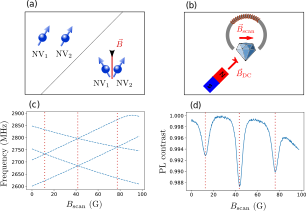
\includegraphics[width=\textwidth]{chapter 3/Figures/NV-NV_equivalent}
\caption{CR between equivalent NV centers for sample ADM-15-1. (a) Representation of equivalent NV centers: either two NVs from the same class, or two classes with the same projected magnetic field. (b) Magnetic setup used for the experiment: a permanent magnet is used to apply a bias magnetic field, and an electromagnet is used to add a variable magnetic field. (c) Simulation of the $\ket{0}\to\ket{-1}$ transition for the 4 classes of NV centers as a function of the scanned magnetic field. The transitions were computed based on several ODMR spectra. The red dotted lines correspond to inter-class resonance (d) Change in the PL of the NV centers ensemble as a function of the scanned magnetic field. The inter-class resonances are reported here.}
\label{equivalent NV-NV}
\end{figure}

More recently, experiments \citep{jarmola2012temperature, mrozek2015longitudinal, jarmola2015longitudinal, choi2017depolarization} on dense NV ensemble ($[\rm NV ] >1\ \rm ppm$) or at low temperature have shown that there were cross-relaxations even between equivalent NV centers.

I refer by equivalent NV centers to NV centers with the same spin Hamiltonian. This means either NV center from the same class, or NV centers from different classes with the same projection of the magnetic field along their axis. Equivalent NV centers are by nature resonant with each other, and therefore susceptible to CR.

Fig. \ref{equivalent NV-NV} shows an experimental observation of equivalent NV-NV CR. The key to observe NV-NV CR is to bring some NV centers in and out of resonance with other NV centers, which we can do with the different NV classes. To do so, we need to add an initial bias magnetic field in addition to the scanned magnetic field, as represented in Fig. \ref{equivalent NV-NV}-b). %When doing so, the magnetic field felt by the diamond won't have a fixed orientation during the scan, and when the magnetic field crosses certain crystalline planes (detailed below), its projection on two or more classes of NV centers will be the same.

Fig. \ref{equivalent NV-NV}-c) shows the transition frequencies of the $\ket{0}\to\ket{-1}$ transition for the 4 classes of NV centers on sample ADM-15-1, an HPHT micro-diamond with $[\rm NV]\sim 3\ \rm ppm$. There are three magnetic field values $B_{\rm scan} \approx$ 12, 42 and 77 G for which there is an inter-class resonance. Each of these resonances correspond to a ``geometric" resonance where the $B$ field is in a symmetry plane between the two classes, meaning that the two resonant NV classes are indeed equivalent.

Finally, Fig. \ref{equivalent NV-NV}-d) shows the PL contrast as the electromagnet field is scanned. There are 3 very clear dips when $B_{\rm scan} \approx$ 12, 42 and 77 G which coincide with inter-class resonances. We will see later that this PL dip is associated with a decrease of the NV centers spin $T_1$ time from both classes.

This observation, and similar ones done by many groups \citep{jarmola2012temperature, mrozek2015longitudinal, choi2017depolarization, akhmedzhanov2017microwave, giri2018coupled}, seem to indicate that there are CR between equivalent NV centers. This is however incompatible with our previous assumptions that equivalent NV centers are equally polarized and bright. To understand this phenomenon, we will need to introduce new hypotheses.

\section{NV inhomogeneity and the fluctuator model}

\subsection{CR in an inhomogeneous NV bath}
\begin{figure}[h]
\centering
\includegraphics[width=\textwidth]{chapter 3/Figures/inhomogene_2_spins}
\caption{a) Schematics of the model: we consider a four level system consisting of 2 levels of 2 NV centers resonantly coupled through the flip-flop rate $\Gamma_{\rm dd}$. These two NV centers are each pumped in their respective $\ket{0}$ state via the green laser with a rate $\Gamma_{\rm las}$, and have their own relaxation rate $\Gamma_1$ and $\Gamma_1^*$ respectively. b) Average population of the two NV centers in the $\ket{0}$ state in the steady state as a function of $\Gamma_{\rm dd}$ and $\Gamma_1^*$. The steady state was computed by solving a classical rate equation where I fixed $\Gamma_{\rm las}=1000\ \rm Hz$ and $\Gamma_1=300\ \rm Hz$.}
\label{inhomogene}
\end{figure}
A likely explanation to the observed NV-NV CR is that the NV centers are not all equivalents.

Indeed, if we assume that, for instance, the relaxation rate $\Gamma_1=1/T_1$ is not strictly the same for each NV centers, but instead follows a certain distribution $\rho(\Gamma_1)$, then CR between NV centers with different $\Gamma_1$ can explain the observations in Fig. \ref{equivalent NV-NV}.

Fig. \ref{inhomogene} illustrates this case. Our model here consists of two NV centers resonantly coupled with two separate relaxation rates $\Gamma_1$ and $\Gamma_1^*$. To complete the model, we add the rate $\Gamma_{\rm las}$ which represent the optical pumping rate from the $\ket{+1}$ to the $\ket{0}$ state of each spin, and $\Gamma_{\rm dd}$ the flip-flop rate between the two spins. We only consider here the incoherent dynamics of the population, modeled with rates. We also only consider the $\ket{0}$ and $\ket{+1}$ states as the results would be the same for the $\ket{0}$ and $\ket{-1}$ states. 

By finding the steady state of these rate equations, we can compute the final population in the $\ket{0}$ for both spins, which we will assume to be proportional to the total PL. Fig. \ref{inhomogene}-b) shows this $\ket{0}$ population as a function of the flip-flop rate $\Gamma_{\rm dd}$ for various values of $\Gamma_1^*$.

We can see that when $\Gamma_1^*=\Gamma_1$, as expected, the PL is not modified by the coupling of the two spins regardless of the coupling strength. When $\Gamma_1^*>\Gamma_1$ however, not only is the starting PL slightly lower since NV$_2$ is less polarized, but the PL now decreases as we increase the coupling strength. This effect, which is at the origin of the CR contrast, is stronger when the difference between $\Gamma_1$ and $\Gamma_1^*$ is important.

\subsection{Presentation of the fluctuator model}
Choi et al. in \citep{choi2017depolarization} take this approach a step further by separating the NV centers into two groups: ``normal" NV centers with a phonon-limited lifetime outside of dipole-dipole interaction, and ``fluctuators" which are NV centers with an intrinsic, extremely fast relaxation mechanism. We are assuming that the fluctuator relaxation rate, $\gamma_f$ is much greater than the optical pumping rate $\Gamma_{\rm las}$. The fluctuators are therefore unpolarized and effectively act as dark spins, similarly to what we discussed in the last chapter.

We should note here that, while this simplifications seem a bit extreme, the fluctuator model is more than a toy model. There are good evidence of the presence of these dark NV centers in dense NV ensemble, as will be discussed below.

We will consider the fluctuators act as a Markovian bath, meaning that the fluctuator density matrix will always read $\rho = \frac{1}{3} I$, regardless of its interaction with NV centers. With this assumption, we can compute the modification caused by the fluctuators on the rest of the NV lifetimes.

Other possibilities to explain the change in the relaxation rate were considered, such as spin diffusion to non-polarized NV centers (outside of the laser spot) or superradiance, but they were not considered to be viable explanations \citep{choi2017depolarization}.
%\begin{pmatrix}
%0.33&0&0 \\
%0&0.33&0 \\
%0&0&0.33
%\end{pmatrix}

\subsection{Single NV center coupled to a single fluctuator}
We will follow here the notations and calculation steps in \citep{choi2017depolarization}. To compute the depolarization induced by the fluctuator bath the NV centers, we should first consider the interaction between a single NV center and a fluctuator. Since we assume the fluctuators to be always depolarized, this step is similar to the coupling of an NV center to a dark spin done in the last chapter.

We will first decompose the dipole-dipole Hamiltonian in a radial and angular part:
\begin{equation}
\mathcal{H}_{\rm dd} \approx - \frac{J_0}{r^3} \left[(g+ih)(\ket{0,+1}\bra{+1,0}+\ket{0,-1}\bra{-1,0}+qS_z^1 S_z^2 \right] + h.c. ,
\end{equation}
where the expression of $J_0, g, h$ and $q$ is given in appendix [REF]. $g, h$ and $q$ are dimensionless factors that are function of the relative position and orientation of the two dipoles.

We then introduce the dimensionless number $\eta$ defined as:
\begin{equation}
\label{eq eta}
\eta^2=\frac{1}{3} (\abs{g}^2+\abs{h}^2)  \frac{4\gamma_f^2}{(\omega_f - \omega_{NV})^2+4\gamma_f^2},
\end{equation}
where $\gamma_f$ is the fluctuator decay rate for each possible channel between $\ket{0}, \ket{-1}$ and $\ket{+1}$. This number $\eta$ encapsulates both the geometry of the problem (through $g$ and $h$) and the resonance condition between the NV center and the fluctuator.

We can note that the spectral response of a single fluctuator, for which we only consider the broadening caused by the decay rate $\gamma_f$, is a Lorentzian of half width $2\gamma_f$. This is different from the usual lifetime limited optical spectra which are Lorentzian of half width $1/2T_1=\Gamma_1/2$. The difference comes here from the fact that we consider thermalization going both ways (i.e. $\ket{e} \to \ket{g}$ and $\ket{g} \to \ket{e}$ instead of only $\ket{e} \to \ket{g}$) and that each state of the fluctuator can decay into two other states.

Finally, the additional depolarization rate induced by the fluctuator on the NV center reads:
\begin{equation}
\gamma_s(\mathbf{r})=\left(\frac{J_0}{r^3}\right) \frac{\eta^2}{\gamma_f}.
\end{equation}
Compared to eq. [REF], the dependency on the inhomogeneous broadening of the spins $1/T_2^*$ is hidden in the $\eta$ factor, and we have the additional broadening $\gamma_f$ coming from the fluctuators very short lifetime.

\subsection{Ensemble of NV centers coupled to a bath of fluctuators}

We now need to compute the average depolarization caused by the ensemble of fluctuators on the ensemble of NV centers.

We consider each fluctuator as in independent depolarization source, therefore the depolarization on a single NV center reads: 
\begin{equation}
\gamma=\sum_i \gamma_s(\mathbf{r}_i).
\end{equation}
We then want to compute the distribution $\rho(\gamma)$ defined as:
\begin{equation}
\rho(\gamma)=\int d\{r_i\} \rho(\{r_i\})\, \delta \left( \sum_i \gamma_s(\mathbf{r}_i) - \gamma \right).
\end{equation}
To do so, we need to determine the distribution of the fluctuators positions and orientations$\{r_i\}$. Assuming that they are homogeneously distributed in the bulk of the material, we find:
\begin{equation}
\rho(\gamma)=\frac{e^{-1/(4\gamma T)}}{\sqrt{4\pi \gamma^3 T}},
\end{equation}
where the time constant $T$ was introduced and is defined as:
\begin{equation}
\frac{1}{T}=\left(\frac{4\pi n_fJ_0\bar \eta}{3}\right)^2 \frac{\pi}{\gamma_f},
\label{eq 1/T}
\end{equation}
with $n$ the fluctuator density and $\bar \eta$ the averaged value of $\abs{\eta}$: 

\begin{equation}
\bar \eta = \int \rm{Prob}(\eta) \abs{\eta} d\eta.
\end{equation}

Finally, the polarization dynamics from the ensemble of NV centers can be computed:
\begin{equation}
P(t)=\int_0^\infty \rho(\gamma)\, e^{-\gamma t}d\gamma= e^{-\sqrt{t/T}}.
\end{equation}

In conclusion, the fluctuators causes a depolarization on the NV ensembles with a timsecale $T$ given by \ref{eq 1/T}, and the dynamics of this depolarization is that of a stretched exponential, unlike the phonon-induced depolarization which is purely exponential. 

It should be noted that the stretched exponential nature of the decay is not proper to the fluctuator model. \citep{hall2016detection} came to the same conclusion by analyzing the resonant coupling of NV centers with a P1 bath. The stretched exponential is a result from localized noise sources, randomly distributed in the bulk (3D).

\subsection{Computation of $\bar \eta$}
\label{sec computation eta}
The parameter $\bar \eta$ in eq. \ref{eq 1/T} is of crucial importance since it encompass the dependence of $1/T$ in both the magnetic field and the inhomogeneous broadening $T_2^*$ of the NV centers and the fluctuators.

We will start by separating the factor $\eta$ given in eq. \ref{eq eta} into a a geometric and a spectral part:
\begin{align}
\eta^2&=G^2(\psi_{NV},\psi_f,\theta,\phi) R^2(\omega_f,\omega_{NV}), \\
G^2&=\frac{1}{3}\left(\abs{g}^2+\abs{h}^2 \right),  \\ 
R^2(\omega_f,\omega_{NV}) &= \frac{4\gamma_f^2}{(\omega_f - \omega_{NV})^2+4\gamma_f^2}.
\end{align}

$G$ is a function which depends purely on the various angles of the problem (angles of the relative position of the NV center and the fluctuator, angle of the NV and fluctuator $z$ axis), while $R$ represents the resonance condition between the NV and the fluctuator.

We will now average this $\eta$ factor for an ensemble of fluctuators and NV centers:
\begin{align*}
\bar \eta &= \int \rm{Prob}(\eta) \abs{\eta} d\eta, \\
&= \left(\int \rho(\psi_{NV},\psi_f,\theta,\phi) |G(\psi_{NV},\psi_f,\theta,\phi)| d\psi_{NV} d\psi_f d\theta d\phi \right) \\
&\, \times \left( \int \rho(\omega_{NV}) \rho(\omega_{f}) |R(\omega_f,\omega_{NV})| d\omega_{NV} d\omega_{f} \right), \\
&= \bar G \cdot \bar R,
\end{align*}
where we introduced $\bar G$ and $\bar R$, the averaging of $|G|$ and $|R|$.

The computation of $\bar G$ will be further discussed in sec. \ref{sec quantitative T1} and in appendix [REF]. We will focus here on $\bar R$.

To perform the computation, we need to know the distributions $\rho(\omega_{NV})$ and $\rho(\omega_{f})$. We can experimentally measure $\rho(\omega_{NV})$ though ODMR, and we can reasonably expect $\rho(\omega_{f})$ to follow the same probability.

We unfortunately cannot analytically solve $\bar R$ for standard distributions of $\rho(\omega_{f})$ and $\rho(\omega_{NV})$ (either Gaussians or Lorentzians). We can however solve $\overline{R^2}$, which is relatively close to $(\bar{R})^2$ as long as $2 \gamma_f \gg 1/T_2^*$.

For a Lorentzian profile of $\rho(\omega_{f})$ and $\rho(\omega_{NV})$ defined as:
\begin{align*}
\rho(\omega_{f})&=\frac{1}{\pi \Gamma_f} \frac{1}{1+ \left(\frac{\omega_f-\omega^0_f}{\Gamma_f}\right)^2} \\
\rho(\omega_{NV})&=\frac{1}{\pi \Gamma_{NV}} \frac{1}{1+ \left(\frac{\omega_{NV}-\omega^0_{NV}}{\Gamma_{NV}}\right)^2},
\end{align*}

where $\Gamma_{f}=1/T_2^*(\rm fluctuator)$ and $\Gamma_{NV}=1/T_2^*(\rm NV)$ are the inhomogeneous broadening of the NV and fluctuator ensemble, and $\omega^0_{NV}$ and $\omega^0_{f}$ are the central angular frequencies of the NV and fluctuator ensemble. We then find that:

\begin{align*}
\overline{R^2}&= \int \rho(\omega_{NV}) \rho(\omega_{f}) \frac{4\gamma_f^2}{(\omega_f - \omega_{NV})^2+4\gamma_f^2} d\omega_{NV} d\omega_{f} \\
&=\frac{2 \gamma_f}{2 \gamma_f + \Gamma_f + \Gamma_{NV}} \cdot \frac{1}{1+\left(\frac{\omega^0_{NV}-\omega^0_{f}}{2 \gamma_f + \Gamma_f + \Gamma_{NV}}\right)^2}.
\end{align*}

In the case where $\omega^0_{NV}=\omega^0_{f}$, meaning that either the considered NVs and fluctuators are from the same class, or from two classes perfectly resonant, by substituting $\overline{R ^2}$ for $(\bar{R})^2$ (which again is only approximately valid for $2 \gamma_f \gg 1/T_2^*$) in eq. \ref{eq 1/T}, we find that:
\begin{equation}
\label{eq 1/T avec T2*}
\frac{1}{T} \propto \frac{1}{2\gamma_f + \Gamma_f + \Gamma_{NV}}.
\end{equation}

If $\rho(\omega_{f})$ and $\rho(\omega_{NV})$ follow Gaussian profiles instead, $\overline{R^2}$ is the integral of a Voigt profile, the convolution of a Lorentzian ans a Gaussian, which does not have a clear analytic solution.

Eq. \ref{eq 1/T avec T2*} is subject to several approximations: the inhomogeneous distribution of the NV centers is generally not Lorentzian, and $\overline{R^2} \neq (\bar{R})^2$ in the general case. Nevertheless, it gives us a general idea of the evolution of $1/T$ with $T_2^*$.

 \subsection{Possible microscopic origin of the fluctuators}

We should note first that a similar problem of spin ensemble relaxation rate increasing with the spin concentration was observed more than six decades ago with phosphorus doped silicon \citep{feher1959electron,honig1960electron}. It was proposed that the cause of the relaxation was the presence of fast relaxing centers coupled to the slow relaxing centers through spin diffusion \citep{honig1960electron, sugihara1963spin, yang1968concentration, vugmeister1978spin, berman2005spin}. 

This conclusion was based on previous observations on the relaxation of nuclear spins \citep{bloembergen1949interaction, de1958relaxation, blumberg1960nuclear}, where some nuclear spins had a considerably reduced lifetime due to their proximity to paramagnetic ions, and also to the resonant energy transfer between molecules \citep{forster1949experimentelle, eisenthal1964influence, yokota1967effects}, where excited donor molecules are coupled through dipole-dipole interaction to non-excited acceptors, and where the stretched exponential dynamics of the donors was first observed \citep{forster1949experimentelle}.

In the case of P-doped Si, the origin of the fast relaxing centers is thought to be closely packed P impurities, so that the electronic wavefunctions of (at least) two P centers overlap. In that case two phenomena occur: the possibility of electron tunneling, and the apparition of a contact interaction term in the dipole-dipole Hamiltonian (see appendix [REF]). Both of these phenomena could lead to fast spin relaxation, the tunneling because the spin hopping can be accompanied by a spin reversal \citep{sugihara1963spin}, and the modulation of the contact interaction strength $J$ by the crystal phonons \citep{honig1960electron}. While the non-contact dipole-dipole interaction is also modulated by the phonons, this effect would be too small to account for the fast depolarization observed here.

Similarly, \citep{choi2017depolarization} suggests that the origin of fluctuators in NV centers are closely packed NV centers or NV-impurity pairs which undergo rapid electron hopping and spin depolarization. To prove their point, they look at the charge dynamics in their sample and find that there is charge recombination in the dark with a corresponding tunneling rate between neighboring sites of $\sim 10\ \rm ns$. In contrast to P-doped Si, the NV centers are not the most abundant electronic defects in the crystal, this is why the NV$^--$N$^+$ pair in particular is thought to be a likely candidate for the fluctuators \citep{manson2018nv}.

\section{Experimental investigation of the fluctuator model}
We will now show experimental results related to the predictions of the fluctuator model.
\subsection{The stretched exponential lifetime}
\begin{figure}[h]
\centering
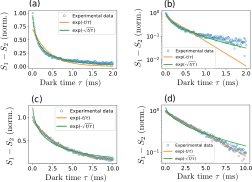
\includegraphics[width=\textwidth]{chapter 3/Figures/Stretch_vs_pas_stretch}
\caption{T1 measurement following the protocol described in [REF]. The best exponential and stretched exponential fits are given each time. a) Sample ADM-15-2 with B=0. The optimal $T_1$ values are $T_1^{\rm stretch}=150\ \mu \rm s$ and $T_1^{\rm exp}=410\ \mu \rm s$. b) Sample CVD-pink with B$\neq$0 and a single class probed. The optimal $T_1$ values are $T_1^{\rm stretch}=1.9\ \rm ms$ and $T_1^{\rm exp}=4.1\ \rm ms$}
\label{stretch_or_not_stretch}
\end{figure}
$T_1$ measurements with dense ensemble of NV centers and when many classes are resonant with each other (typically when B=0) indeed tend to show stretched exponential profiles.

Fig. \ref{stretch_or_not_stretch} shows an example of that: in Fig. \ref{stretch_or_not_stretch}-a) the $T_1$ measurement comes from sample ADM-15-2 at B=0. The profile is clearly better fitted by a stretched exponential than a regular exponential, and the timescale found $T_1^{\rm stretch}=150\ \mu \rm s$ is much shorter than the expected phonon limite lifetime of a few ms.

On the other hand, Fig. \ref{stretch_or_not_stretch}-b) shows a $T_1$ measurement coming from sample CVD-pink for B$\neq$0. This time the profile is more exponential, and the value $T_1^{\rm exp}=4.1\ \rm ms$ is coherent with a phonon-limited lifetime. Even though the sample CVD-pink shows some NV-NV CR feature, the spin dynamics in this sample is still dominated by the phonons, which explains the exponential profile.


\subsection{Fitting $T_1$ profile in the general case}

\begin{figure}[h]
\centering
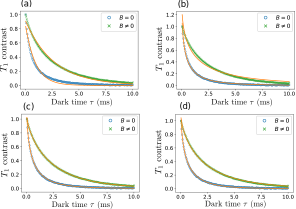
\includegraphics[width=\textwidth]{chapter 3/Figures/various_fit_formulae}
\caption{Different fitting procedure on two $T_1$ measurements done on sample ADM-150-1 for $B=0$ and $B\neq0$. \\ a) Exponential fit $S(\tau)=\exp (-\tau/T_1^{\rm ph})$. \\ b) Stretched exponential fit $S(\tau)=\exp (-\sqrt{\tau/T_1^{\rm dd}})$. \\ c) Bi-exponential fit $S(\tau)=\exp (-\tau/T_1^{\rm ph} -\sqrt{\tau/T_1^{\rm dd}})$. \\ d) Bi-exponential fit with fixed $T_1^{\rm ph}=5\ \rm ms$: $S(\tau)=\exp (-\tau/5 -\sqrt{\tau/T_1^{\rm dd}})$.}
\label{various_fit_formulae}
\end{figure}

\begin{table}[htbp]
\centering
\caption{Fitting parameters for Fig.
 \ref{various_fit_formulae}}
 \label{fitting table}
\begin{tabular}{c|cc|cc}
\toprule
Figure &  \multicolumn{2}{c}{$B=0$} & \multicolumn{2}{c}{$B\neq0$}\\
\midrule
{} &  $T_1^{\rm ph}$ (ms)& $T_1^{\rm dd}$ (ms)&  $T_1^{\rm ph}$ (ms)& $T_1^{\rm dd}$(ms)\\
Fig. a) & 0.95 & * & 2.64 & * \\
Fig. b) & * & 0.32 & * & 1.03  \\
Fig. c) & 6.75 & 0.44 & 4.22 & 7.19 \\
Fig. d) & \textbf{5} & 0.51 & \textbf{5} & 4.65 \\
\bottomrule
\end{tabular}

Bold characters indicate parameters that were arbitrarily fixed.
\end{table}

For many samples however, the $T_1$ profile is neither fully exponential nor fully stretched exponential, because the relaxation time associated with CR, which we will call $T_1^{\rm dd}$ is of the same order as the phonon limited lifetime $T_1^{\rm ph}$. Sometimes the same sample can go from mostly exponential to mostly stretched exponential depending on the number of NV-NV co-resonances, forcing us to include both aspects if we want a unique fitting formula.

Fig. \ref{various_fit_formulae} shows four different fitting procedure on the two same experimental data. The data here are two $T_1$ measurements done on the same sample ADM-150-1, following the protocol described in [REF], with and without an external magnetic field ($\sim 50 G$). The magnetic field was strong enough to split the four classes and only one class was probed in the case $B\neq0$ , whereas all 4 classes were resonant in the case $B=0$, which strongly increases the NV-NV CR. 

The fits used here are either purely exponential or purely stretched exponential, or a combination of both where the exponential lifetime $T_1^{\rm ph}$ was either left as a free parameter or fixed at a value $T_1^{\rm ph}=5\ \rm ms$. The values of the different fitting parameters used is reported in Table \ref{fitting table}.

We can see that neither the purely exponential nor stretched exponential fits can be satisfying for both measurements: the $B=0$ curve is poorly fitted by the exponential fit and the $B \neq 0$ curve is poorly fitted by the stretched exponential. The protocols that include both exponential and stretched lifetimes correctly fit both curves. In the case of Fig. \ref{various_fit_formulae}-d), we arbitrarily fixed $T_1^{\rm ph}=5\ \rm ms$ since this is the value we typically measure on samples with low NV density, and we expect that the phonon-limited exponential lifetime is not modified by the NV concentration.

Since the protocol where $T_1^{\rm ph}$ was fixed and the one where it wasn't both correctly fit our data, we decided to use the protocol where $T_1^{\rm ph}$ was fixed because there is one less free parameter in the fitting function, and the values we obtain on $T_1^{\rm dd}$ can be directly compared. 

We should note however that the values of $T_1^{\rm dd}$ we obtain are not absolute. Indeed, in the case of Fig. \ref{various_fit_formulae}, the value of $T_1^{\rm ph}$ can be somewhat arbitrarily fixed between 3 and 6 ms with satisfying fits, and the resulting values $T_1^{\rm dd}$ can vary by almost an order of magnitude in the case of $B\neq0$. While this technique of measuring $T_1^{\rm dd}$ is useful to compare different cases, because it is fairly sensitive, it is not an exact measurement of the dipole-dipole induced lifetime.

\begin{figure}[h]
\centering
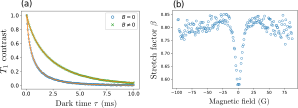
\includegraphics[width=\textwidth]{chapter 3/Figures/betas}
\caption{a) Same two measurements as Fig. \ref{various_fit_formulae} with the fitting formula $S(\tau)=\exp ((-\tau/T_1)^{\beta})$. The fitting parameters are $\beta=0.58$ and $T_1=0.46\ \rm ms$ for $B=0$, and $\beta=0.80$ and $T_1=2.15\ \rm ms$ for $B\neq0$. b) Optimal $\beta$ parameter found for each $T_1$ measurement as a function of the external magnetic field (still on sample ADM-150-1).}
\label{betas}
\end{figure}

Finally, another fitting procedure is shown in Fig. \ref{betas}. This time we are using a single stretched exponential with an arbitrary stretch factor $\beta$. Fig. \ref{betas}-b) shows the optimal $\beta$ parameter as a function of the external magnetic field. We can then confirm that the $T_1$ profile gets closer to a stretched exponential ($\beta=0.5$) when $B$ goes to 0. 

Even though this method also yields satisfying fits, it needs two free parameters to work ($\beta$ and $T_1$), so we decided to go with the method of Fig. \ref{various_fit_formulae}-d) instead.

\subsection{The fluctuators linewidth}

\subsubsection{The fluctuators spectral response}
\begin{figure}[h]
\centering
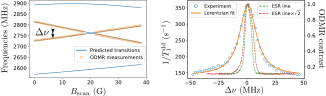
\includegraphics[width=\textwidth]{chapter 3/Figures/fluctuator linewidth}
\caption{Measurement of the fluctuators linewidth on sample ADM-150-2 using the same setup as in Fig. \ref{equivalent NV-NV}. a) Simulation of the $\ket{0} \to \ket{-1}$ transition frequency for the four classes of NV centers and actual frequencies of the two central classes from ODMR measurements. b) Measurement of $T_1^{\rm dd}$ as a function of the splitting $\Delta \nu$ between the two central classes, fitted with a Lorentzian of half-width $\sigma=8.78\ \rm MHz$. The green dashed line correspond to the ODMR spectrum of a single class of NV centers, and the red dashed one to the same line scaled up by a factor $\sqrt{2}$}
\label{fluct linewidth}
\end{figure}



One of the main arguments in favor of the fluctuator model is the measurement of the fluctuators spectral response. Indeed, as we will see, the fluctuator lifetime is so short that it significantly broadens the fluctuators spectral response compared to standard NV centers.

The fluctuator are effectively dark to ODMR measurement since they are not polarized, but we can measure their linewidth through CR the same way we would do for a dark spin, as detailed in \citep{hall2016detection}.

Fig. \ref{fluct linewidth} shows an experiment similar to the one presented in Fig. \ref{equivalent NV-NV}. A variable magnetic $B_{\rm scan}$ in addition to an offset magnetic field $B_{\rm DC} \sim 100\ \rm G$ are used in order to create a crossing between two classes of NV centers, but this time measuring the spin decay rate instead of the PL.

Fig. \ref{fluct linewidth}-a) shows the simulated transitions of the four classes of NV centers as a function of the magnetic field, and the experimentally measured central frequencies of the two classes of interest when the two lines can be clearly separated. Having a precise measurement of the detuning between the two classes $\Delta \nu$ is key in this experiment to get a precise value of the fluctuator linewidth.
%Because the $T_1$ measurement protocol described in [REF] requires a resonant microwave pulse with the NV probed, we specifically record ODMR spectra of their two central lines to get a precise measurement of the Larmor frequency. In the region where the two ODMR lines overlap we have to use a linear regression to get the Larmor frequency of each class.

Fig. \ref{fluct linewidth}-b) shows the dipole-dipole induced relaxation rate $\Gamma_1^{\rm dd}=1/T_1^{\rm dd}$ as a function of the detuning $\Delta \nu$ between the two central classes. For each magnetic field value, a $T_1$ profile was recorded and fitted following the procedure described in Fig. \ref{various_fit_formulae}-d) where we again fixed $T_1^{\rm ph}=5\ \rm ms$. We also show the ODMR spectrum of a single NV class for comparison.

We can clearly see that the $\Gamma^{\rm dd}$ profile is much broader than the ODMR line of the NV centers, whereas in a standard CR process, we expect the decay rate to be proportional to the spectral overlap of the two classes \citep{hall2016detection}. If we assume that both NV classes spectral response are gaussians of same width $\sigma$, then the spectral overlap between the two classes is also a gaussian of width $\sqrt{2} \sigma$. Fig. \ref{fluct linewidth}-b) also shows the ODMR line scaled by a factor $\sqrt{2}$, which is still much narrower than the $1/T_1^{\rm dd}$ line.

We attribute this broadening to the fluctuators lifetime. Another potential explanation for the broadening could be the interaction strength between the NV center and the fluctuator, but for [NV] $\sim$ 5 ppm, the average dipole-dipole coupling strength between closest NV neighbor is $\expval{\mathcal{H}_{\rm dd}} \sim 46\ \rm kHz$, which cannot explain the $\sim 4\ \rm MHz$ broadening that we observe.

\subsubsection{The fluctuators lifetime}
\begin{figure}[h]
\centering
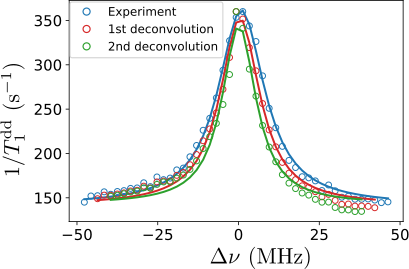
\includegraphics[width=0.6\textwidth]{chapter 3/Figures/deconvolution}
\caption{Blue curve $1/T_1^{\rm dd}$ data presented in Fig. \ref{fluct linewidth}. Red curve: deconvolution of the blue curve the  by the ODMR line shown on the same figure. Green curve: deconvolution of the red curve the  by the ODMR line. All three curves are fitted with Lorentzian of respective half widths 8.78, 7.49 and 6.38 MHz}
\label{deconvolution}
\end{figure}

We now want to extract the fluctuators lifetime $T_1^f=1/\gamma_f$ to get further information on their potential nature. 

To do this we first assume that the dipole induced decay rate is proportional to the overlap of the spectral responses of the NV centers and fluctuators $S_{NV}$ and $S_f$. We will take $S_{NV}( \omega)$ and $S_{f}( \omega)$ as functions centered in $\omega=0$, and consider that the spectral responses are shifted by $\omega^0_{NV}$ and $\omega^0_{f}$ respectively, the central frequencies of each group. We then have:
\begin{align*}
\frac{1}{T_1^{\rm dd}} &\propto \int S_{NV} (\omega-\omega_{NV}^0) S_f (\omega-\omega_{f}^0) d\omega \\
&= \int S_{NV} (\omega-\Delta \omega) S_f (\omega)
 d\omega \\
 &= (S_{NV}*S_{f})(\Delta \omega),
\end{align*}

where $\Delta \omega=\omega_{NV}^0-\omega_{f}^0$.

Using the approximation $\bar {R ^2} \approx (\bar{R})^2$ detailed in sec. \ref{sec computation eta}, we can then decompose the fluctuator spectral response between the lifetime contribution and the inhomogeneous broadening:
\begin{equation}
S_{f}(\omega)=\left(S_f^*(\omega)\right)*\left(\frac{1}{1+\left(\frac{\omega}{2 \gamma_f}\right)^2} \right),
\end{equation}

where $S_f^*$ is the spectral broadening caused by the inhomogeneous distribution of the fluctuators, which we will suppose to be equal to $S_{NV}$. With these assumptions, we are now ready to extract $\gamma_f$ from the data of Fig. \ref{fluct linewidth}.

The first way to do this, as was done for NV-P1 CR in \citep{hall2016detection}, is to deconvolve the $1/T_1^{\rm dd}$ data by the ODMR spectrum using a Wiener deconvolution algorithm. The result of the deconvolution is shown in Fig. \ref{deconvolution}: the data is deconvolved once to get the spectral response of the fluctuator (red curve), and a second time to get only the lifetime contribution of the fluctuator (green curve). Fitting with Lorentzians, we find a final value $\Gamma_2 =2\gamma_f= (2\pi) 6.38\ \rm MHz$ which corresponds to a fluctuator lifetime $T_1^f=\frac{1}{\gamma_f}=49.9\ \rm ns$.

Another, simpler alternative is to consider that the $1/T_1^{\rm dd}$ profile is a Voigt profile given by the convolution of two Gaussians of half width at half maximum (HWHM) $f_G=\frac{\sqrt{\ln (2)}}{\pi T_2^*}$ and a Lorentzian of HWHM $f_L=\frac{2 \gamma_f}{2 \pi}$:
\begin{align*}
\Gamma_1^{\rm dd}&\propto \mathcal{G}(f_G)*(\mathcal{L}(f_L)*\mathcal{G}(f_G)) \\
&\propto \mathcal{L}(f_L)*\mathcal{G}(\sqrt{2} f_G),
\end{align*}
where $\mathcal{G}(f_G)$ and $\mathcal{L}(f_L)$ denote Gaussian and Lorentzian functions of HWHM $f_G$ and $f_L$ respectively.
We can then use the formula of a pseudo-Voigt profile which gives an approximation of the Voigt profile's HWHM $f$ as a function of $f_G$ and $f_L$ \citep{ida2000extended}:
\begin{equation}
f = [f_G^5 + 2.69269 f_G^4 f_L + 2.42843 f_G^3 f_L^2 + 4.47163 f_G^2 f_L^3 + 0.07842 f_G f_L^4 + f_L^5]^{1/5}.
\end{equation}

With $f=8.78\ \rm MHz$ and $\sqrt{2}f_G=4.33\ \rm MHz$, we find $f_L=6.54\ \rm MHz$ for a final lifetime value $T_1^f = 48.7\ \rm ns$, a value consistent with the one found with the deconvolution method.

Doing similar calculations, \citep{choi2017depolarization} found $\gamma_f=1/T_1^f=(2\pi) 3.3\ \rm MHz$ which gives them a fluctuator lifetime value $T_1^f = 48.2\ \rm ns$, a value surprisingly similar to the one we got.


\section{Resonance between several NV classes}

The main tool to probe NV-NV CR is to use the co-resonances between the NV classes. While it is not possible to completely shut down the CR, because the NV centers from the same class are always resonant with each other, we can tune the density of resonant NV centers (and supposedly resonant fluctuators) by a factor of 4 by playing with the inter-class co-resonances. We will discuss here the various scenarios where NV classes overlap, and the quantitative impact it has on the centers' spin $T_1$.

\subsection{Geometric conditions for inter-class resonance}

\begin{figure}[h!]
\centering
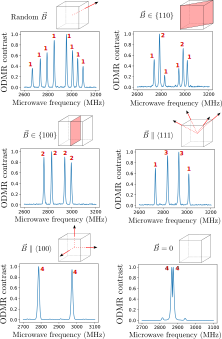
\includegraphics[width=0.8\textwidth]{chapter 3/Figures/Resonance_geometries}
\caption{ODMR spectra on sample ADM-15-3 as a function of the magnetic field orientation. The field amplitude is $\sim 60\ \rm G$. Red numbers represent the number of resonant classes for each ODMR line. The cubes represent the diamond unit cell, and the red planes/arrow the possible orientations of the magnetic field}
\label{ODMR_geometries}
\end{figure}

There are four possibilities to obtain inter-class resonance (outside of the non-equivalent CR discussed in sec. \ref{non_equi_valent_CR}). These possibilities are:
\begin{itemize}
\item $\mathbf{B} \in \{110\}$. We refer by $\{110\}$ as any plane orthogonal to a $\langle 110 \rangle$ or equivalent direction. In this magnetic configuration, two classes are at resonance and the two other ones are spectrally isolated.
\item $\mathbf{B} \in \{100\}$. In this magnetic configuration, the four classes form two pairs of co-resonance.
\item $\mathbf{B} \parallel \langle 111 \rangle$. In this configuration discussed in the last chapter, one class is aligned with the magnetic field and is spectrally isolated while the three other form a resonant triplet.
\item $\mathbf{B} \parallel \langle 100 \rangle$. In this configuration also discussed in the last chapter, the four classes are resonant.
\end{itemize}
We should add to this list the case $\mathbf{B}=0$ where all four classes are also resonant, and any other possibility (which I will call random $\mathbf{B}$) where all four classes are spectrally separated. 

An ODMR spectrum and a representation of the magnetic field in the diamond unit cell for each of these six possibilities is shown in Fig. \ref{ODMR_geometries}.

\begin{figure}[h]
\centering
\includegraphics[width=\textwidth]{chapter 3/Figures/carte}
\caption{PL contrast as a function of the magnetic field polar and azimuthal angle with respect to the [100] axis on sample CVD-pink. The field amplitude is $\abs{B} \sim 115 G$. The locus of the magnetic field in specific planes is noted by red dashed lines.}
\label{Carte}
\end{figure}

This relation between NV-NV class resonances and the magnetic field being in specific crystalline planes or directions means that we can determine the crystal main axes simply by PL experiments.

Fig. \ref{Carte} shows a map where we simply monitored the PL of sample CVD-pink while scanning the magnetic field angle around the [001] axis, thanks to a permanent magnet on a motorized goniometer. We have also reported the locus of $\mathbf{B}$ being in the planes [100], [010], [110] and [$1\bar 1 0$].

We know that when $\mathbf{B}$ belongs to any of these four planes, there is a co-resonance between at least two NV classes. This co-resonance leads to an increase in NV-NV CR and a faster depolarization of the spins involved, which ultimately leads to a drop in PL. We can indeed see in fig. \ref{Carte} that there is clear correlation between the loci of $\mathbf{B}$ and drops in PL. We can also see that the PL is at its lowest when $\mathbf{B}\parallel [001]$, which corresponds to a four class degeneracy.

\subsection{Quantitative modification of $T_1$}
\label{sec quantitative T1}
\begin{table}[htbp]
\centering
\caption{Theoretical and experimental values of $\Gamma_1^{\rm dd}=1/T_1^{\rm dd}$ for various magnetic field configurations, expressed as a function of the value found for an isolated class. The experimental values were measured on sample ADM-15-3 using the protocol of Fig. \ref{various_fit_formulae}-d) with $T_1^{\rm ph}= 5\ \rm ms$.}
 \label{T1 champ mag}
\begin{tabular}{c|cc}
\toprule
$\Gamma_1^{\rm dd} (\mathbf{B})$ &  Theory & Experimental \\
\midrule
random $\mathbf{B}$ (1 class) & $\Gamma_0^{\rm th}$ & 1.53 ms$^{-1} \equiv \Gamma_0^{\rm exp}$ \\
$\mathbf{B} \in \{110\}$ (2 classes) & 10.0 $\Gamma_0^{\rm th}$ & 5.20 $\Gamma_0^{\rm exp}$ \\
$\mathbf{B} \in \{100\}$ (2 classes) & 7.24 $\Gamma_0^{\rm th}$ & 4.22 $\Gamma_0^{\rm exp}$ \\
$\mathbf{B} \parallel \langle 111 \rangle$ (3 classes) & 28.4 $\Gamma_0^{\rm th}$ & 9.07 $\Gamma_0^{\rm exp}$ \\
$\mathbf{B} \parallel \langle 100 \rangle$ (4 classes) & 42.8 $\Gamma_0^{\rm th}$ & 11.3 $\Gamma_0^{\rm exp}$ \\
$\mathbf{B}=0$ (4 classes) & 51+($^*$) $\Gamma_0^{\rm th}$ & 15.4 $\Gamma_0^{\rm exp}$ \\
\bottomrule
\end{tabular}

($^*$) The case $\mathbf{B}=0$ will be detailed in the next chapter. The theoretical value is a lower bond.
\end{table}

The fluctuator model allows quantitative predictions of the change in the spin lifetime, thanks to eq. \ref{eq 1/T}. There are however several unknown in this equation, such as the fluctuator density and lifetime which can be hard to estimate. It is however relatively easy to compare the predictions of eq. \ref{eq 1/T} for various magnetic field configurations.

What we decided to do was to take the case of an isolated class, where we consider that NV centers from said class or only affected by fluctuators of the same class, as the baseline value for the dipole-dipole decay rate $\Gamma_0$, and to express the decay rates when 2,3 or 4 classes are co-resonant as a function of $\Gamma_0$. Doing so allows to normalize $n_f$ and $\gamma_f$ in eq. \ref{eq 1/T} and to keep $\bar G$ the geometrical part of $\bar \eta$ as the only unknown.

$\bar G$ can be analytically or numerically computed for each of the magnetic configurations listed before, as detailed in appendix [REF]. This allows us to predict the value of the spin decay rate in every situations as a function of the decay rate of an isolated class.

Table \ref{T1 champ mag} shows these predicted values, along with experimental ones on sample ADM-15-3. The experimental values were obtained with the protocol described in Fig. \ref{various_fit_formulae}-d) with a double exponential fit where we fixed again $T_1^{\rm dd}=5\ \rm ms$.

The theoretical values are in a good qualitative agreement with the experimental ones, both ranking the different scenarios in the same order. The quantitative predictions of the theory however are rather poor, being off by more than a factor of 3 for the shortest lifetimes.

It should be noted that the experimental values were heavily influenced by the choice of the parameter $T_1^{\rm ph}$. Using for example $T_1^{\rm ph}=2.5\ \rm ms$ gave results closer to the theoretical ones. Nevertheless, the fluctuator model generally tends to overestimate the depolarization rates.The authors of \citep{choi2017depolarization} for instance found that a 2-class degeneracy (the authors did not precise whether this was a $\mathbf{B} \in \{110\}$ or $\mathbf{B} \in \{100\}$ configuration) yielded an increased depolarization rate by a factor $\sim 4$, a value comparable to the one we found in table \ref{T1 champ mag}, and two times smaller than the predicted one. We can also see in Fig. \ref{fluct linewidth} that a $\mathbf{B} \in \{110\}$ configuration leads to a $\sim 2.5$ times increase in $\Gamma_1^{\rm dd}$, 4 times smaller than the predicted factor of 10.

The failure of the fluctuator model to accurately predict the changes in $T_1$ is one of the reasons that led us to believe that the model is incomplete.

\section{Conclusion and perspectives}

In conclusion, we have seen in this chapter that dense NV ensemble present ``anormal" CR between the NV centers, and we have shown how the fluctuator model developed by Choi et al. in \citep{choi2017depolarization} can explain this behavior. The fluctuator model not only explains the NV-NV CR, but also correctly predicts the stretched exponential lifetime profile. It also correctly predicts that the fluctuators have a broader spectral response than the other NV centers. Nevertheless, the model does not describe perfectly every aspects of NV-NV relaxation, and there still are many aspects of this problem, both theoretical and experimental, to explore.

In what follows I will describe what I think would be interesting investigation points to further understand the NV-NV relaxation and the fluctuator model.

\subsection{Limitations of the fluctuator model}
\begin{figure}[h]
\centering
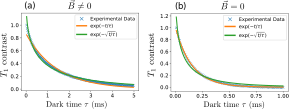
\includegraphics[width=\textwidth]{chapter 3/Figures/Anormal_T1}
\caption{$T_1$ measurements on sample ADM-15-4, fitted with pure exponential or stretched exponential. a) $T_1$ of a single isolated class when $\mathbf{B} \neq 0$. The optimal fit parameters are respectively $T_1^{\rm exp}=1.43\ \rm ms$ and $T_1^{\rm stretch}=0.56\ \rm ms$. b) $T_1$ of the four degenerate classes when $\mathbf{B}=0$. The optimal fit parameters are respectively $T_1^{\rm exp}=0.15\ \rm ms$ and $T_1^{\rm stretch}=0.05\ \rm ms$.}
\label{anormal T1}
\end{figure}

I already mentioned that the discrepancy between the theoretical and experimental $T_1$  values were an issue of the current fluctuator model, although the difference could come in part from the $T_1$ fitting procedure. Another, more glaring problem is the fact that some $T_1$ profile are not stretched exponential.

Fig. \ref{anormal T1} shows $T_1$ measurement on sample ADM-15-4, either on a single isolated class ,where the dipole-dipole interactions are at their weakest, or on all four resonant classes at $\mathbf{B}=0$, where the interactions are at their strongest.

For the single isolated class, the $T_1$ profile seems to be closer to a stretch exponential, which is coherent with the fact that the lifetime $T_1 \sim 1\ \rm ms$ is already smaller than the expected phonon limited lifetime $T_1^{\rm ph} \sim 5\ \rm ms$. However when $\mathbf{B}=0$, although the lifetime gets $\sim$ 10 times shorter, the profile becomes clearly exponential. 

The spin dynamics in this sample is still dominated by resonant dipole-dipole interactions: the more classes are brought to resonance, the shorter the spin $T_1$. But here, the profile gets closer to a pure exponential when $T_1$ decreases, which is in complete contradiction with the fluctuator model.

This particular sample was a 15 $\mu$m micro-diamond, which could have a role in this observation since we know that spins near the surface have a reduced $T_1$ \citep{rosskopf2014investigation}, and micro-diamonds have proportionally more near surface spins. But other diamonds from the same batch, such as the one measured in Fig. \ref{stretch_or_not_stretch}, show clearly stretched exponential profile in the same conditions, and meanwhile some bulk diamonds show very short non-stretched exponential lifetimes, similar to the present sample.

It seems therefore that the current fluctuator model does not correctly describe the spin dynamics of every NV-dense samples. Looking at what was previously done for P-doped SI \citep{vugmeister1978spin} or for resonant energy transfer between molecules \citep{yokota1967effects}, the fluctuator model could probably be improved by taking into account the finite lifetime of the fluctuators (i.e. the saturation of the NV-fluctuator CR), and the spin diffusion between NV centers (the fluctuator model only considers NV-fluctator interactions and not NV-NV interactions).

\subsection{Investigation of the fluctuators nature}
While the hypothesis of fluctuators being clusters of NV centers or NV-other spins is solidified by the precedents in P-doped Si \citep{honig1960electron} or F centers in KCl \citep{warren1964spin}, there are still many unknowns on the exact nature of the fluctuators. There are at least two aspects that I think merit to be investigated.

The first one would be to study the fluctuator spectral profile on various samples showing NV-NV CR. In particular it would be interesting to know whether this profile is always Lorentzian, and what its linewidth is. In the sample I studied on Fig. \ref{fluct linewidth}, I found a value for $\gamma_f$ surprisingly similar to the one found in \citep{choi2017depolarization}, even tough my sample only had $[\rm NV] \sim 3 ppm$ compared to the $[\rm NV] \sim 45 ppm$ sample used in \citep{choi2017depolarization}. If $\gamma_f$ was found to be somewhat of a constant among all samples showing NV-NV CR, this would give us a lot of information on the potential nature of the fluctuators. Studying the temperature dependency of $\gamma_f$ could also give us information on whether the depolarization mechanism is due to tunneling or modulation of the $J-$coupling by the phonons.

The other aspect would be to identify potential defects that could form fluctuators when paired with NV centers. The main candidate for this would be substitutional nitrogen (P1 or P1$^+$ centers) since they are the most abundant electronic spin species in the diamond we use. The ideal way to confirm this hypothesis would be to compare the spin $T_1$ for  different samples with the same [NV] concentration, but different [P1] concentration. If indeed P1 centers play a role in the presence of fluctuators, we would expect a shorter NV $T_1$ time in the sample with high P1 concentration.


\printbibliography
\end{refsection}
 \begin{refsection}

\chapter{NV-NV CR under transverse or low fields: application to magnetometry}

In the last chapter we saw how dense ensemble of NV centers have an intrinsic depolarization mechanism mediated by the NV-NV dipole interaction. In this chapter we will see how this feature can be exploited to perform magnetometry. 

Using NV-NV CR for magnetometry in non-zero magnetic field has already been proposed \citep{akhmedzhanov2017microwave, akhmedzhanov2019magnetometry}. We will focus here on the low to zero magnetic field region, which presents practical advantages as the relative orientation of the diamond with the magnetic field does not need to be controlled, but theoretical complications due to the more complex physics of the NV centers under low magnetic field.

This chapter is constructed as follows: We will first describe the physics of NV centers under low or transverse magnetic field (the physics is similar in both cases), we will then show both theoretically and experimentally that the NV-NV CR is modified for low and transverse magnetic field. We will identify different mechanisms by which the relaxation is modified and we will try to quantify their relative importance.

We will then focus on the low field depolarization magnetometry (LFDM) protocol which exploits the previously studied NV-NV CR at low magnetic field. We will start by giving a short overview of NV ensemble magnetometry before characterizing the LFDM protocol and comparing it to other magnetometry protocols. Finally we will give some perspectives on how to improve LFDM and on potential applications.

The results presented in this chapter are based in large part on the article \citep{pellet2022spin}.

\section{NV spin Hamiltonian under low and transverse fields}

Before looking at the NV-NV CR in the low or transverse field regime, we first need to consider how the general NV physics is modified under those regimes, and in particular we need to look at the modifications of the spin Hamiltonian and the change in the eigenstates compared to the high magnetic field regime.

\subsection{NV spin Hamiltonian in zero external magnetic field}
\begin{figure}[h]
\centering
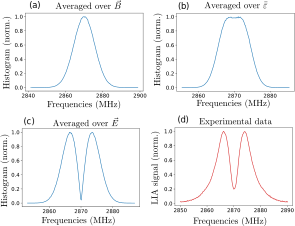
\includegraphics[width=\textwidth]{chapter 4/Figures/ESR_simus}
\caption{Simulations of inhomogeneous zero field ODMR when sampling various parameters. a) Simulation when sampling each components of the magnetic field over a Gaussian of deviation $\sigma=2\ \rm G$. b) Simulation when sampling each components of the strain tensor $\bar{\bar{\varepsilon}}$ over a Gaussian of deviation $\sigma=2\cdot 10^{-4}$. c) Simulation when sampling each components of the electric field over a Gaussian of deviation $\sigma=2\cdot 10^{5}\ \rm{V/cm}$. d) Experimental ODMR spectrum in zero external field taken on sample ADM-150-2}
\label{simus ESR}
\end{figure}

In the absence of external magnetic field, we have to take into account other elements which would otherwise be of second order in the spin Hamiltonian. These elements are: the random local magnetic fields caused by paramagnetic impurities, the local electric field caused by charged impurities, and the crystal strain \citep{doherty2012theory, udvarhelyi2018spin, mittiga2018imaging}. The hyperfine splitting due to nearby nuclei will be considered separately, although to a large extent it behaves like a local magnetic field.

Due to the large zero field splitting $D=2870\ \rm MHz$ between the $\ket{0}$ and $\ket{\pm 1}$ states, we will consider the $\ket{0}$ state to always be an eigenstate of the spin Hamiltonian under zero external field (which is equivalent to say that we neglect the terms in $\ket{0}\bra{\pm 1}$ in the spin Hamiltonian). The problem is then reduced to the $\{ \ket{-1}, \ket{+1} \}$ subsystem.

The NV$^-$spin Hamiltonian in the $\{ \ket{-1}, \ket{+1} \}$ basis can be written as \citep{udvarhelyi2018spin}:
\begin{equation}
\mathcal{H}=\begin{pmatrix}
D-\gamma_e B_\parallel + f_\parallel(\mathbf{E}) + g_\parallel(\bar{\bar{\varepsilon}}) & f_\perp(\mathbf{E}) + g_\perp(\bar{\bar{\varepsilon}})\\
f^*_\perp(\mathbf{E}) + g^*_\perp(\bar{\bar{\varepsilon}})&D+\gamma_e B_\parallel + f_\parallel(\mathbf{E}) + g_\parallel(\bar{\bar{\varepsilon}})
\end{pmatrix},
\label{Hamiltonien pm1}
\end{equation}
where $B_\parallel$ is the component of the magnetic field along the NV axis, and $f_\parallel, f_\perp, g_\perp$, and $g_\parallel$ are functions of the electric field $\mathbf{E}$ and the strain tensor $\bar{\bar{\varepsilon}}$, whose expressions are:

\begin{align}
f_\parallel(\mathbf{E})&=d_\parallel E_z, \\
f_\perp(\mathbf{E})&=d_\perp ( E_x + i E_y), \\
g_\parallel(\bar{\bar{\varepsilon}})&= h_{41}(\varepsilon_{xx}+\varepsilon_{yy})+h_{43} \varepsilon_{zz}, \\
g_\perp(\bar{\bar{\varepsilon}}) &= \frac{1}{2} \left[ h_{16}(\varepsilon_{zx}+i \varepsilon_{zy}) + h_{15}\left(\frac{\varepsilon_{yy}-\varepsilon_{xx}}{2}+i\varepsilon_{xy}\right) \right],
\end{align}
where $d_\parallel=0.35 \ \rm{Hz\, cm/V}$ and $d_\perp=17\ \rm{Hz\, cm/V}$ have been measured experimentally \citep{van1990electric}, and $h_{43}=2300\ \rm{MHz}$, $h_{41}=-6420\ \rm{MHz}$, $h_{15}=5700\ \rm{MHz}$ and $h_{16}=19660\ \rm{MHz}$ were computed through DFT \citep{udvarhelyi2018spin} and show reasonable agreement with experiments \citep{barson2017nanomechanical}.

Importantly, as pointed in \citep{mittiga2018imaging} we notice that both the electric field and the strain have a \textit{shifting} component ($f_\parallel$ and $g_\parallel$) which shifts equally both eigenstates of the Hamiltonian, and a \textit{splitting} component ($f_\perp$ and $g_\perp$) which splits in energy the two eigenstates. 

The main difference between the electric field and the strain is in the numerical prefactors of these components: for the electric field, the splitting parameter $d_\perp$ is $\sim 50$ times higher than the shifting parameter $d_\parallel$, which will result on average to a strong energy split without much shifting. For the strain however, the splitting parameters $h_{15}$ and $h_{16}$ are only $\sim 3$ times higher than the shifting parameters $h_{43}$ and $h_{41}$. The shift in energy will therefore tend to blur the energy split when averaging over a large number of spins.

Fig. \ref{simus ESR} shows a simulation of how each parameters of the spin Hamiltonian - local magnetic field, local electric field and strain - affects the zero external field ODMR profile. To do these simulations, I sampled each parameters separately $10^6$ times and plotted the histogram of the two eigenvalues of the Hamiltonian written in eq. \ref{Hamiltonien pm1}. Fig. \ref{simus ESR}-d) shows an experimental zero field ODMR spectrum, typical of what we observe with dense NV ensembles. 

Experimentally, almost all our samples show the characteristic two bumps in zero external field ODMR. Given the simulation results, the only parameter that can give rise to this shape is the local electric field. 

We should note that another potential explanation for the splitting of the $\ket{\pm 1}$ states could be the presence of a residual magnetic field, not randomly distributed among all the spins but homogeneous on the whole sample. In particular, we do not shield for the earth magnetic field in our experiment. The splitting caused by the earth magnetic field however has a value $\gamma B_{\rm earth} \approx 1\ \rm MHz$, which is $\sim 4$ times weaker than the splitting we typically observe. 

We will therefore consider that the low external magnetic field spin Hamiltonian of our samples is dominated by the local electric field, and more specifically by the transverse electric field $E_\perp\equiv E_x + i E_y$ given the ratio between $d_\perp$ and $d_\parallel$.

We will then adopt the following simplified Hamiltonian for the zero external field regime:
\begin{equation}
\mathcal{H}=\begin{pmatrix}
D&0&d_\perp E_\perp^* \\
0&0&0 \\
d_\perp E_\perp &0&D
\end{pmatrix},
\end{equation}
whose eigenvectors are $\ket{0}$ and$\ket{\pm}$ of eigenvalues 0 and $D\pm d_\perp \abs{E_\perp}$, where $\ket{\pm}$ are defined as:
\begin{equation}
\ket{\pm}=\frac{\ket{+1}\pm e^{-i\phi_E}\ket{-1}}{\sqrt{2}},
\end{equation}
where $\tan(\phi_E)=E_y/E_x$.

\subsection{NV spin Hamiltonian under purely transverse magnetic field}
\label{sec B transverse}
%\begin{figure}[h]
%\centering
%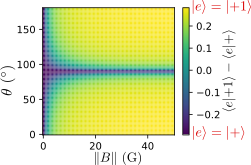
\includegraphics[width=0.7\textwidth]{chapter 4/Figures/map_etats_propres}
%\caption{Closeness of the Hamiltonian most excited state $\ket{3}$ with either $\ket{+1}$ or $\ket{+}$ as a function of the external magnetic field amplitude and angle $\theta$ with respect to the NV axis.}
%\label{map champ transverse}
%\end{figure}

We now turn to the case of purely transverse magnetic field with respect to the NV axis, i.e. $\mathbf{B}=B_x \hat{e}_x + B_y \hat e_y$, and more specifically to the regime where $d_\perp E_\perp < \frac{(\gamma_e B_\perp)^2}{D} << D$. In practice, this generally corresponds to $20\ \rm G \lesssim B_\perp \lesssim 200\ \rm G$.

In this regime, the NV Hamiltonian eigenstates are similar to the case where it is dominated by the transverse electric field and can be written $\approx \ket{0}, \ket{-}, \ket{+}$\citep{qiu2021nuclear, qiu2022nanoscale}, of respective eigenvalues $\approx -\frac{(\gamma_e B_\perp)^2}{D},D,D+\frac{(\gamma_e B_\perp)^2}{D}$,  where:
\begin{equation}
\ket{\pm}=\frac{\ket{+1}\pm e^{-2i\phi_B}\ket{-1}}{\sqrt{2}},
\end{equation}
and $\tan(\phi_B)=B_y/B_x$.

For the case where $d_\perp E_\perp \sim \frac{(\gamma_e B_\perp)^2}{D}$ and $\phi_E \neq 2\phi_B$, the eigenstates of the Hamiltonian are still of the form $\ket{0},\ket{\pm}$ with a relative angle $\phi$ in between $\phi_E$ and $2\phi_B$.

In conclusion, whenever the spin Hamiltonian is dominated by a transverse field, either electric or magnetic, we can consider that the eigenstates of the spin Hamiltonian to be $\ket{0}, \ket{-}$ and $\ket{+}$, whereas when the Hamiltonian is dominated by the longitudinal magnetic field, its eigenstates are $\ket{0}, \ket{-1}$ and $\ket{+1}$.

\subsection{Hyperfine coupling and inhomogeneous broadening}
\label{sec modif T2*}
\begin{figure}[h]
\centering
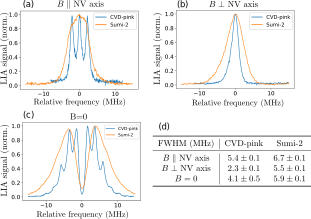
\includegraphics[width=\textwidth]{chapter 4/Figures/Comparaison_ESR_T2}
\caption{ODMR lineshapes for longitudinal, transverse and low magnetic fields on samples CVD-pink and Sumi-2. a) ODMR spectrum of a single class of NV centers for a longitudinal magnetic field ($B_\parallel \sim 100\ \rm G$). The microwave frequency is given with respect to the ODMR line central frequency. b) ODMR spectrum of a single class for a purely transverse magnetic field ($B_\perp \sim 100\ \rm G$). c) ODMR of all 4 classes for 0 external magnetic field. d) Table reporting the full width at half maximum of each ODMR line.}
\label{ESR for T2*}
\end{figure}

We will now look at the modification in the ODMR linewidths caused by the different magnetic field regimes. These change are relevant to our study of NV-NV CR due to the relation between the dipole-induced relaxation rate and $T_2^*$ detailed in sec. [REF].

A consequence of the change in the Hamiltonian eigenstates from the $\{ \ket{0}, \ket{\pm 1} \}$ to the $\{ \ket{0}, \ket{\pm} \}$ basis is that the Hamiltonian eigenvalues are sensitive to different part of the environment. In the $\{ \ket{0}, \ket{\pm 1} \}$, the eigen energies are linearly sensitive to (longitudinal) magnetic field, and only sensitive to electric fields at the second order, and vice versa for the $\{ \ket{0}, \ket{\pm} \}$ basis.

These different sensitivities affect both the inhomogeneous broadening, due to the local electric and magnetic noise, and the hyper-fine coupling to the various surrounding nuclei. These effects can drastically modify the ODMR lineshape in zero external magnetic field \citep{jamonneau2016competition} or purely transverse magnetic field \citep{qiu2021nuclear,qiu2022nanoscale}.

We will only consider here the hyper-fine splitting caused by the $^{14}$N nuclei of the nitrogen atom forming the NV center. $^{14}$N represents 99.6 \% of natural abundance nitrogen atoms, and it has an $I=1$ nuclear spin. The full $3\times 3$ Hamiltonian of the NV center in these conditions can be written:
\begin{equation}
\mathcal{H}=\mathcal{H}_e + \mathcal{H}_n + \mathbf{S} \bar{\bar{A}} \mathbf{I},
\end{equation}

where $\mathbf{S}$ is the electronic spin operator, $\mathbf{I}$ the nuclear spin operator, $\mathcal{H}_e$ the previously described electronic spin Hamiltonian, $\mathcal{H}_n$ the nuclear spin Hamiltonian and $\bar{\bar{A}}$ the hyper fine tensor. $\mathcal{H}_n$ and $\bar{\bar{A}}$ can be written:

\begin{equation}
\mathcal{H}_n = \gamma_N \mathbf{I} \cdot \mathbf{B} + Q I_z^2,
\end{equation}

and
\begin{equation}
\bar{\bar{A}} = \begin{pmatrix}
A_{xx} & 0 & 0 \\
0 & A_{yy} & 0 \\
0 & 0 & A_{zz}
\end{pmatrix},
\end{equation}


where $\gamma_N=0.308\ \rm kHz/G$, $Q=-4.945\ \rm MHz$, $A_{zz}=-2.162\ \rm MHz$ and $A_{xx}=A_{yy}=-2.62\ \rm MHz$ \citep{smeltzer2009robust}.

Fig. \ref{ESR for T2*} shows ODMR spectra for two samples, CVD-pink and Sumi-2, in three magnetic configuration: for a strong longitudinal magnetic field, where the NV eigenbasis is $\{ \ket{0}, \ket{\pm 1} \}$, and for a strong transverse magnetic field or no magnetic field, where the NV eigenbasis is $\{ \ket{0}, \ket{\pm} \}$. 

While both samples are relatively equivalent in term of NV concentration ([NV]=$3 \sim 5$ ppm), sample Sumi-2 contains significantly more impurities besides NV centers, most likely P1 centers. These impurities cause both magnetic (because of paramagnetic impurities) and electric (because of charged impurities) field noise.

Fig. \ref{ESR for T2*}-a) allows us to evaluate the magnetic field noise in both samples, since the $\ket{\pm 1}$ states are not sensitive to weak electric fields. We indeed find that the Sumi-2 sample has much more magnetic noise, to the point where the hyper-fine structure is no longer resolved. The total width of the line however is mostly dominated by the hyper-fine splitting, which result in a similar total linewidth in both cases

We should note that the usual practice in magnetometry is to consider the linewidth only of the three hyper-fine lines when they are resolved. This is because magnetometry protocol usually relies on a microwave field with a very well defined frequency, which can effectively select only one of the lines. In our case however, we have to consider the spectral overlap between NV centers and fluctuators, which have an additional broadening of $2\gamma_f \approx 6\ \rm MHz$ [REF] that completely obscures the hyper-fine structure. We therefore have to consider the full linewidth, even when the hyper-fine structure is resolved.

Fig. \ref{ESR for T2*}-b) allows us to evaluate the electric field noise in both samples, since the $\ket{\pm}$ states are not sensitive to weak magnetic fields. Similarly, the hyper-fine structure is hidden in this configuration since all three hyper-fine levels are nearly-degenerate, provided that $\frac{(\gamma_e B_\perp)^2}{D} > A_{xx},A_{zz},Q$ which is typically the case for $B_\perp > 40\ \rm G$. We can note that the electric field noise is significantly stronger in sample Sumi-2, which leads to an ODMR linewidth more than twice as big.

Finally, \ref{ESR for T2*}-c) shows the linewidth of both samples for zero external magnetic field. For sample Sumi-2, the profile and linewidth is similar to the case of the purely transverse magnetic field, which is consistent with the fact that the electric field noise is stronger than the residual magnetic fields (earth magnetic field and hyper-fine interaction). For sample CVD-pink however, the electric field noise is smaller than the hyper-fine interaction, meaning that only the $\ket{m_s=-1,m_I=+1}$ and $\ket{m_s=+1,m_I=-1}$ states (the ones closest to the central dip) will be dominated by the electronic noise, and be in the electronic states $\ket{m_e=\pm}$. The $\ket{m_I=\pm 1}$ states are dominated by the hyper-fine field and are in the electronic $\ket{m_e=\pm 1}$ basis.

The table in Fig. \ref{ESR for T2*}-d) reports the linewidths measured on both sample for the various magnetic field configurations. We can see that the linewidth of sample CVD-pink varies by more than a factor of 2, while the ones from sample Sumi-2 varied by less than 20 \%. We should note that  almost all samples used in this chapter are HPHT type 1b diamond, similar to sample Sumi-2 and unlike sample CVD-pink. We should therefore expect the modification of $T_2^*$ to have a moderate impact on the depolarization dynamics.

\medskip

To summarize this section, we have seen that (for the samples used in this chapter) the NV centers spin Hamiltonian is dominated by transverse electric field for low external magnetic field, and that it causes a change of the Hamiltonian eigenstates from $\{ \ket{0}, \ket{\pm 1} \}$ to $\{ \ket{0}, \ket{\pm} \}$. We have seen that the Hamiltonian has the same eigenstates for a purely transverse magnetic field, and finally we have seen that this change of eigenstates occasion a modification of the spins $T_2^*$, although this modification is slight for samples with a high impurity density.

\section{NV-NV CR in the low magnetic field regime}
In this part, we will study the cross-relaxation between NV centers under low magnetic field, whose spin Hamiltonian is dominated by a transverse electric field. Understanding the various mechanisms operating in this regime will be important for the magnetometry protocol presented after.

\subsection{Experimental observations}
\begin{figure}[h]
\centering
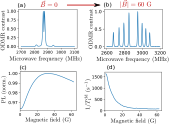
\includegraphics[width=0.9\textwidth]{chapter 4/Figures/scan_1x1x1x1}
\caption{Low field depolarization on sample ADM-150-1 for $\mathbf{B}$ in an arbitrary direction. a) ODMR spectrum for B=0. b) ODMR spectrum for B=60 G. c) PL contrast as a function of the external magnetic field. d) $1/T_1^{\rm dd}$ as a function of the external magnetic field. A $T_1$ measurement was recorded for each magnetic field value and fitted accorded to the protocol described in [REF] with $T_1^{\rm ph}=5\ \rm ms$}
\label{scan 1x1x1x1}
\end{figure}
We will start by showing that NV-NV CR behaves differently in the low magnetic field regime compared to the longitudinal field dominated regime which we studied in the last chapter.

The main issue with studying NV-NV CR in low to zero magnetic field is that there are many competing effects happening simultaneously, with few buttons to adjust in order to isolate each effects.

Fig. \ref{scan 1x1x1x1}-c) and d) show the evolution of the NV PL and stretched lifetime $T_1^{\rm dd}$, defined in the last chapter [REF], as the magnetic field is scanned from 0 to 60 G. The ODMR at the initial and final magnetic fields are shown in Fig. \ref{scan 1x1x1x1}-a) and b).

While it is clear that the spin lifetime as well as the PL increases with the magnetic field, there is no clear indication that this is because of the specificity of the low field region. Indeed, the most likely explanation in this case is that the four classes of NV centers get split apart as the magnetic field increases, which reduces the density of resonant fluctuators for each NV centers. 

We can note however that the PL is not an exact mirror of the spin dynamics: while the low field drop in PL is indeed associated with a reduced spin lifetime, the drop in PL at higher magnetic field comes from the states mixing induced by the transverse magnetic field, and is not associated with a modification of the spin dynamics (to the first order).

\begin{figure}[h]
\centering
\includegraphics[width=0.9\textwidth]{chapter 4/Figures/scan_100}
\caption{Same measurements as Fig. \ref{scan 1x1x1x1}, still on sample ADM-150-1, but with $\mathbf{B}$ along the [100] axis.}
\label{scan 100}
\end{figure}

Fig. \ref{scan 100} presents a way to circumvent this issue: by applying the magnetic field along the [100] crystalline axis, we can make sure that the four classes of NV centers always stay resonant regardless of the magnetic field amplitude.

We can notice that there still is a decrease of both the PL and $T_1^{\rm dd}$ in low field, although considerably smaller than the previous case: in Fig. \ref{scan 1x1x1x1}, $T_1^{\rm dd}$ was reduced by a factor of $\sim$ 8 in zero field, whereas in Fig. \ref{scan 100}, it was only reduced by a factor of $\sim$ 1.2. The main reason for the PL and $T_1$ drop in Fig. \ref{scan 1x1x1x1} was indeed the co-resonance between the four classes.

Nevertheless, the fact that there is a drop in zero field when $\mathbf{B} \parallel [100]$ cannot be explained if we consider only the inter-class resonances. This means that there are some additional depolarization mechanisms which are proper to the zero field region. We should also note that, while the zero-field PL contrast is bigger in Fig. \ref{scan 1x1x1x1}-c) than in Fig. \ref{scan 100}-c), the PL slope, which is the limiting factor for sensing ability, is actually similar in both cases.

We can also note a drop in PL and a corresponding increase of $1/T_1^{\rm dd}$ for $B \sim 20\ \rm G$ which corresponds to the NV$-^{13}$C-NV cross-relaxation discussed in [REF]

\subsection{Theory of the low field depolarization}
\label{sec causes zero field}
We have identified three possible reasons for the zero field depolarization observed in Fig. \ref{scan 100}. Once presented, we will try to hierarchized the contribution of each of these effects.

\subsubsection{Eigenstates modification}
The first explanation is the modification of the dipole-dipole interaction caused by the change of the NV Hamiltonian eigenbasis from $\{ \ket{0}, \ket{\pm 1} \}$ when $\mathbf{B} \neq 0$ to $\{ \ket{0}, \ket{\pm} \}$ when $\mathbf{B} = 0$.

This modification arise from the new form of the dipole-dipole Hamiltonian in the $\{ \ket{0}, \ket{+}, \ket{-} \} \times \{ \ket{0}, \ket{+}, \ket{-} \}$ basis. We justify this change of basis, where we only considered the single NV Hamiltonian instead of the full two-spins Hamiltonian, by the fact that we are in the weak coupling regime, where $\expval{\mathcal{H}_{dd}} \approx 50\ \rm kHz \ll \frac{1}{2\pi T_2^*} \approx 5\ \rm MHz$ meaning that we can treat the dipole-dipole interaction perturbatively. To compute the decay rate with these new eigenstates, we now need to consider the $\mel{0,\pm}{\mathcal{H}_{dd}}{\pm ,0}$ matrix elements instead of the $\mel{0,\pm 1}{\mathcal{H}_{dd}}{\pm 1,0}$ ones.

The computation of the decay rates in the new eigenbasis involve the averaging of these matrix elements which is detailed in appendix [REF]. The computation in this case is complicated by the fact that the transverse field (either $\mathbf{E}$ or $\mathbf{B}$) responsible for the splitting of the $\ket{\pm}$ levels breaks the Hamiltonian symmetry in the $(xy)$ plane. This means that the dipole-dipole coupling between two spins will depend on their relative $x$ and $y$ axis, defined by the local transverse field, on top of the relative $z$ axis defined by the NV axis. 

We therefore need to make an assumption on the distribution of the transverse field in the sample. In zero external magnetic field where the dominant transverse field comes from randomly spaced charged impurities, we can expect the $x$ and $y$ axes to be randomly sampled in their respective $(xy)$ plane. However, since the NV-fluctuator CR is dominated by the closest neighbor of each spin (due to the $1/r^6$ scaling in eq. [REF]), there could still be local correlations in the transverse field felt by the NV and its nearest fluctuator.

We then computed the decay rates for the two extreme cases: first, we consider that the $x$ and $y$ axis of each spin is randomly sampled, which correspond to a correlation length of the transverse field $l_c=0$, and secondly we considered the case where the dominant transverse field as a fixed orientation in the whole sample corresponding to $l_c=\infty$.

We found for $\mathbf{B}=0$ that the expected decay rate was $\Gamma_1=51.4 \Gamma_0^{\rm th}$ if $l_c=0$ and $\Gamma_1=55.0 \Gamma_0^{\rm th}$ if $l_c=\infty$. $\Gamma_0^{\rm th}$ has the same definition as in table [REF], it is the expected decay rate for an isolated class in the $\{ \ket{0}, \ket{\pm 1} \}$ basis.

In both cases, this is a moderate ($\sim 20 \%$) increase compared to $\Gamma_1=42.8 \Gamma_0^{\rm th}$ which we previously found for $\mathbf{B} \parallel [100]$, where all four classes were degenerate but the Hamiltonian eignebasis was $\{ \ket{0}, \ket{\pm 1} \}$. The change in the Hamiltonian eigenbasis for low field is therefore a possible candidate to explain the low field depolarization in Fig. \ref{scan 100}

\subsubsection{Double flips}

\begin{table}[htbp]
\centering
\caption{Simulated depolarization rate for flip-flops and double flips in zero magnetic field}
 \label{table double flips}
\begin{tabular}{c|cc}
%\toprule
{} & $l_c=0$ & $l_c=\infty$ \\
\midrule
$\bar{R}^2=1$ & $126.8 \Gamma_0^{\rm th}$ & $126.8 \Gamma_0^{\rm th}$ \\
$\bar{R}^2=0.5$ & $93.7 \Gamma_0^{\rm th}$ & $95.4 \Gamma_0^{\rm th}$ \\
$\bar{R}^2=0$ & $51.4 \Gamma_0^{\rm th}$ & $55 \Gamma_0^{\rm th}$ \\
%\bottomrule
\end{tabular}
\end{table}

Another effect which happens only at low magnetic field is the possibility of double flip between the NV center and the fluctuator, which is the simultaneous flip of both spins in the same directions, for example going from $\ket{0,-1}$ to $\ket{+1,0}$. The processes $\ket{0, \pm 1}\bra{\mp 1,0}$ are resonant for $B=0$ and not anymore when the degeneracy between the $\ket{\pm 1}$ states is lifted by the magnetic field.

We have seen however that for weak magnetic fields the eigenstates of each NV Hamiltonian are $\ket{\pm}$ and not $\ket{\pm 1}$, due to the transverse electric field. And the $\ket{+}$ and $\ket{-}$ states are not resonant in zero magnetic field. But we can see from Fig. \ref{simus ESR}-d) or \ref{ESR for T2*}-c) that the splitting $2 d_\perp E_\perp \approx 8\ \rm MHz$ is of the same order than the $1/T_1^{\rm dd}$ profile of linewidth $\Gamma^{\rm dd} \approx 8.8\ \rm MHz$ measured on Fig. [REF]. In zero external magnetic field, the $\ket{+}$ and $\ket{-}$ states are therefore close enough in energy that double flip can take place.

To compute the depolarization induced by the double flips, we need to add another decay channel in the fluctuator model, on top of the flip-flop one. We also need to take into account the fact that the $\ket{+}$ and $\ket{-}$ states are not fully resonant, which will modify the $\bar{R}$ factor defined in [REF]. Finally, the question about the correlation  length of the electric field also needs to be asked.

The results are summed up in Table \ref{table double flips}. We again give the results for the two extreme cases regarding the correlations in the electric field, and we show three possible scenario regarding the pseudo-resonance of the $\ket{+}$ and $\ket{-}$ states, represented by the $\bar{R}^2$ factor: $\bar{R}^2=1$ means that the states are fully resonant ($\omega_+-\omega_- \ll \Gamma^{\rm dd} $), this would be the maximum possible decay rate involving the double flips. $\bar{R}^2=0.5$ represents the case where the splitting between the states is equal to the fluctuator linewidth ($\omega_+-\omega_- \approx \Gamma^{\rm dd}$). This is close to the the experimental values we have. Finally $\bar{R}^2=0$ correspond to the case where the states are too far detuned for the double flips ($\omega_+-\omega_- \gg \Gamma^{\rm dd} $). We come back to the results of the last section where only considered the flip-flops.


\subsubsection{$T_2^*$ modification}

The last aspect we considered was the change in $T_2^*$ (we include the change in the hyper-fine interaction in the $T_2^*$) for weak magnetic field, as discussed in sec. \ref{sec modif T2*}.

To quantify its impact in the depolarization rate, we employ eq. [REF], where we use the values $2\gamma_f = 6.5\ \rm MHz$ estimated in the last chapter and we take for $\Gamma_f=\Gamma_{\rm NV}$ the values of half width at half maximum found in Fig. \ref{ESR for T2*}. 

We then find that the modification of $T_2^*$ should increase the decay rate in zero field by $\sim 9 \%$ for sample Sumi-2, and by $\sim 24 \%$ for sample CVD-pink. 


\subsubsection{Summary}
\begin{figure}[h]
\centering
\includegraphics[width=\textwidth]{chapter 4/Figures/Shema_summary_theory}
\caption{Visual summary of the different depolarization effects in low magnetic field and their predicted depolarization rate}
\label{summary_theory}
\end{figure}

Fig. \ref{summary_theory} recapitulate the various mechanisms at play in the low field depolarization of NV ensemble. 

We start from from the simplest case where every classes are sepctrally isolated and the only dipole-induced relaxation coms from the flip-flop between NV and fluctuators from the same class. We then consider the case where all four classes are resonant ($B\parallel [100]$) and finally the case B=0.

The three extra depolarization mechanisms in zero field are then detailed, with the predicted increase of depolarization rate for each step. The predicted rates in zero field depend on several parameters, we chose the following ones to compute the different numerical values: $l_c=0$, $\bar{G}^2=0.5$, $2\gamma_f = 6.5\ \rm MHz$ and $2/T_2^*=5.9\ \rm MHz$ (corresponding to sample Sumi-2 if we assume a Lorentzian ODMR profile).

\subsection{Other potential causes for zero field depolarization}
We have also considered two other potential causes that we have ultimately ruled out in this case.

\subsubsection{Magnetic field alignment}
\begin{figure}[h]
\centering
\includegraphics[width=.7\textwidth]{chapter 4/Figures/alignement_rose}
\caption{PL of sample CVD-pink as a function of the magnetic field for various misalignment of the field direction with the [100] axis}
\label{alignement rose}
\end{figure}

The first is a potential misalignment of the magnetic field with the [100] axis, which would cause a splitting of the 4 classes as the magnetic field increases. This hypothesis is not consistent with the observations in Fig. \ref{scan 100}-d): we would expect a small  misalignment to cause a slow but steady decrease of $1/T_1^{\rm dd}$ as the magnetic field is increased. Instead we observe a sharp decrease followed by a pseudo-plateau.

We still estimated how sensitive the PL dip was with respect to the field alignment. Fig. \ref{alignement rose} shows PL scans on sample CVD-pink for various alignment of the magnetic field around the [100] axis. We estimate our alignments to be precise within $\pm 1^\circ$. We can see that the central feature is almost unaffected by the orientation within [$-3^\circ$:$+3^\circ$] which confirms that the low field depolarization does not come from a field misalignment.

\subsubsection{Laser polarization}
\begin{figure}[h]
\centering
\includegraphics[width=.7\textwidth]{chapter 4/Figures/pola_laser}
\caption{PL of sample ADM-150-3 with respect to the magnetic field for various laser polarization angle. The magnetic field orientation was chosen arbitrarily in the plane of polarization of the laser field}
\label{pola laser}
\end{figure}

Other studies \citep{anishchik2015low, filimonenko2020weak} previously saw a correlation between the zero magnetic field PL dip and the polarization angle of the laser with respect to the magnetic field. 

Fig. \ref{pola laser} shows PL scans on sample ADM-150-3 for various polarization angle of the incident laser. We chose to apply the magnetic field in the laser polarization plane, in a direction that did not match any particular crystalline planes.

We can see no clear differences between the different polarization angles used, whereas \citep{anishchik2015low} and \citep{filimonenko2020weak} saw an antiline growing inside the PL dip when $B \perp E_{\rm las}$. We think that the difference between our experiments come from the fact that we are using denser NV ensembles, and that any effects tied to the laser polarization are hidden by the stronger effects discussed previously.


\section{NV-NV CR under purely transverse magnetic field}
We have seen in the last part that there was a spontaneous spin depolarization specifically in zero external magnetic field, and we have identified three potential mechanisms which are the double-flips, the change in the Hamiltonian eigenstates and the modification of $T_2^*$. We now want to experimentally discriminate the contribution of each of these mechanisms and to see how close the actual decay rates are to the predicted ones. 

One of the reason we want to separate these contributions is that they scale differently with the different variables of the sample ($T_2^*$, $\gamma_f$ , magnetic and electric noise ...). Understanding which of these effect dominates the zero field dynamics might give us insight on which parameter to optimize if one wants to avoid the zero field depolarization, or on the contrary to increase it.

The ideal way to isolate each contributions would be to apply an electric field strong enough to split the transition of the 4 classes, and to measure the decay rate of a single class dominated by the transverse electric field. Such an electric field would need to be of the order of $\sim 10^6\ \rm{V/cm}$, which is several order of magnitudes greater than the breakdown voltage of air and out of our experimental reach.

Instead of an electric field, we will use a transverse magnetic field, which as described in sec. \ref{sec B transverse} leads to a spin Hamiltonian similar to the one where the transverse electric field dominates, or at least to similar eigenstates.

\subsection{Principle of the experiment}
\begin{figure}[h]
\centering
\includegraphics[width=\textwidth]{chapter 4/Figures/transis_transverse_field}
\caption{Simulation of the eigenstates of the NV Hamiltonian for  a purely transverse magnetic field $B_\perp$. In addition to the transverse magnetic field, we consider a fixed transverse electric field of value $d_\perp E_\perp=4\ \rm MHz$. (a) Eigenvalues for the spin Hamiltonian as a function of $B_\perp$. The three states are labeled $\ket{1}$, $\ket{2}$ and $\ket{3}$. (b) Splitting between the $\ket{2}$ and $\ket{3}$ states (blue curve) and closeness factor $\abs{\bra{3}\ket{+}}^2$ between the $\ket{3}$ and $\ket{+}$ (red curve)}
\label{eigenstates transverse field}
\end{figure}

Fig. \ref{eigenstates transverse field} shows a simulation of the eigenstates and eigenenergies for a NV Hamiltonian subject to transverse electric field and magnetic field. For convenience we chose to take $E_\perp = E_x$ and $B_\perp = B_x$, taking other geometric configuration alters only slightly the results. We labeled the eigenstates of the Hamiltonian $\ket{1}$, $\ket{2}$ and $\ket{3}$ in ascending order of energy.

Fig. \ref{eigenstates transverse field}-b) shows both the splitting $\Delta \nu$ between the $\ket{2}$ and $\ket{3}$ states, and how close the $\ket{3}$ state is to the $\ket{+}=\frac{\ket{+1}+\ket{-1}}{\sqrt{2}}$ state via the factor $\abs{\bra{3}\ket{+}}^2$. We look at the $\ket{3}$ state since $\ket{2}=\ket{-}=\frac{\ket{+1}-\ket{-1}}{\sqrt{2}}$ in this case.

These two metrics, $\Delta \nu$ and $\abs{\bra{3}\ket{+}}^2$ are what we are interested in: we want to increase $\Delta \nu$ to the point where the double flips are completely quenched, but we want $\abs{\bra{3}\ket{+}}^2$ to remain close to 1 since we wanted to observe the modification caused by the eigenbasis $\{\ket{0},\ket{\pm}\}$. This way we can isolate the $T_1^{\rm dd}$ contribution coming from the change of eigenstates to the one coming from the double flips. Based on the plots in Fig.\ref{eigenstates transverse field}-b), the region with $B_\perp \in$ [100,200] G seems to satisfy both these criteria.

\subsection{Experimental data}

\begin{figure}[h!]
\centering
\includegraphics[width=.8\textwidth]{chapter 4/Figures/scan_T1_perp}
\caption{Experimental data for the depolarization under purely transverse magnetic field on sample ADM-150-2. a) ODMR spectrum for $|\mathbf{B}|=20\ \rm G$. The transitions of the class orthogonal to the magnetic field are labeled $\nu_+$ and $\nu_-$. b) Dependency of $\nu_+$ and $\nu_-$ with the magnetic field, as measured through ODMR. c) Measurement of $T_1^{\rm dd}$ as a function of the transverse magnetic field. The corresponding energy splittings $\Delta \nu=\nu_+-\nu_-$ are written on top. We divided the plot between the A region where $1/T_1^{\rm dd}$ decreases, and the B region where it reaches a plateau with a value $1/T_1^{\rm dd}=185 \pm 5\ \rm s^{-1}$ indicated by a red line. We also indicate in green the value found for a purely longitudinal magnetic field $1/T_1^{\rm dd}=126 \pm 10\ \rm s^{-1}$}
\label{champ tranverse exp}
\end{figure}

We perform here a $T_1^{\rm dd}$ measurement similar to the one presented in Fig. [REF], on the same sample and with the same fitting parameters, but this time probing a class orthogonal to the magnetic field.

Fig. \ref{champ tranverse exp}-a) and b) show the evolution of the transition frequencies $\nu_+=\frac{E_{\ket{3}}-E_{\ket{1}}}{h}$ and $\nu_-=\frac{E_{\ket{2}}-E_{\ket{1}}}{h}$ where $\ket{1}$, $\ket{2}$ and $\ket{3}$ are the states described in Fig. \ref{eigenstates transverse field}. The magnetic field was scanned between 20 and 130 G by increment of $\sim 0.5\ \rm G$.

Fig. \ref{champ tranverse exp}-c) shows the evolution of $1/T_1^{\rm dd}$ with the magnetic field. We have denoted two region: in region A, $1/T_1^{\rm dd}$ decreases with the magnetic field, from a value of $350\ \rm s^{-1}$ to a value of $185\ \rm s^{-1}$. In region B, the value of $1/T_1^{\rm dd}$ is stable and does not decrease further when $B_\perp$ is increased.

\subsubsection{Region A}

We attribute the decrease in region A to the double flips: as the magnetic field increases, so does $\Delta \nu$ and the double flips become less and less resonant to the point where they become completely quenched for $B_\perp \approx 90\ \rm G$ or $\Delta \nu \approx 30\ \rm MHz$. This value is coherent with the previously measured fluctuator linewidth. We can then estimate the part of the double flips in the total depolarization rate for the low field regime (20 G here) and find that they amount for $\sim 50\%$ in this case.

Another possibility to explain this drop could be that the class orthogonal to $\mathbf{B}$ still exerts flip-flops with the other classes at low magnetic field, as we can see in Fig. \ref{champ tranverse exp}-a) that they are not very far detuned. However we have to consider that the detuning between the two states $\nu_+-\nu_-= 9\ \rm MHz$ is significantly lower, even at $B_\perp=20\ \rm G$, than the detuning with the closest class $\nu_\pm-\nu_{\rm other}= 22\ \rm MHz$; and also that there seem to be a small plateau for $1/T_1^{\rm dd}$ at the beginning of region A which is consistent with the double flip hypothesis since  $\nu_+-\nu_-$ is almost flat in this region while $\nu_\pm-\nu_{\rm other}$ increases linearly with the magnetic field.

\subsubsection{Region B}

We now turn to region B. Even tough the double flips are completely quenched, the effects of the eigenbasis modification and the $T_2^*$ reduction are still present, because we can see on Fig. \ref{eigenstates transverse field}-b) that the eigenstates of the spin Hamiltonian are still very close to $\{ \ket{0}, \ket{\pm} \}$ for these magnetic field values.

To evaluate the contribution of the eigenbasis and $T_2^*$, we measure the same class of NV centers, but this time with a longitudinal magnetic field ($B_\parallel \sim 100 G$) to get a baseline value of $1/T_1^{\rm dd}$ in the $\ket{\pm 1}$ basis. We found a value of $1/T_1^{\rm dd}=126 \pm 10\ \rm s^{-1}$ in this case, reported on Fig. \ref{champ tranverse exp}-c) as a green line. 

We do find that the decay rate is higher in the $\ket{\pm}$ basis by $\sim 50\% $ which corroborates our predictions, as both the change of eigenbasis from $\ket{\pm 1}$ to $\ket{\pm}$ and the increase of $T_2^*$ in the $\ket{\pm}$ basis are predicted to increase the depolarization rate. The theoretical increase however overestimates once again the actual increase: for the change of eigenbasis alone we predicted an increase of the decay rate by a factor of 4 (see appendix [REF]), over 8 times more than the actual increase.

We unfortunately cannot experimentally discriminate the depolarization coming from the eigenbasis change or the $T_2^*$ while using the same sample, since both of this properties are tied to the Hamiltonian eigenstates. But we do know that in this scenario, for a single isolated class, the contribution of both the change of eigenbasis and $T_2^*$ amounts for $\sim 3$ times less than the double flips. 

\subsubsection{Conclusion of the experimental observation}

We have here quantitatively measured different depolarization contributions for a single class submitted to purely transverse magnetic field, and we expect that the depolarization for low magnetic fields behave similarly. We therefore claim that the difference in NV polarization between the $\mathbf{B}=0$ region and $\mathbf{B} \neq 0$ region is caused by (in order of importance):
\begin{enumerate}
\item The lift of degeneracy between the four classes caused by the projection of the magnetic field on the different NV axis.
\item The double flips between the nearly resonant $\ket{+}$ and $\ket{-}$ states at low magnetic field.
\item The change of the Hamiltonian eigenbasis from $\{\ket{0}, \ket{\pm} \}$ in the electric field dominated region to $\{\ket{0}, \ket{\pm 1} \}$ in the magnetic field dominated region, and the incident change in $T_2^*$.
\end{enumerate}

\section{Introduction to ensemble NV magnetometry}

Before we explore the application of low field depolarization to magnetometry, we must discuss the general field of NV magnetometry. 

NV magnetometry is generally decomposed between single NV and ensemble magnetometry. Single NVs,often associated with scanning probes, offer a spatial resolution limited only by how far the magnetic source can be from the NV center (typically $\sim 10\ \rm nm$), but at the cost of a relatively low sensitivity (typically $\sim \mu \rm{T} / \sqrt{\rm Hz}$ \citep{pelliccione2016scanned}).

Ensemble NV centers center on the other hand offer sensitivities as low as $1\ \rm pT / \sqrt{\rm Hz}$ \citep{wolf2015subpicotesla}, at the cost of working with samples of sizes up to several mm.

We will only focus here on NV ensemble magnetometry since we want to give elements of comparisons with our technique based on NV-NV CR. We will not try to give a complete overview of this field, but only of the elements close to the technique we present. For a general overview on NV magnetometry, we recommend the excellent reviews  \citep{rondin2014magnetometry, degen2017quantum, barry2020sensitivity}.

\subsection{AC and DC magnetometry}
The most sensitive NV magnetometry protocols use the free precession of the spins to map a small change in the Zeeman energy into the phase of the spins, which is then converted into spin population. These protocols are generally distinguished between DC-broadband and AC-narrow band.

For DC-broadband magnetometry, the general technique consist of a Ramsey interferometry experiment, presented in chapter 1, which is limited by the spin inhomogeneous coherence time $T_2^* \lesssim 1\ \rm{\mu s}$ for NV ensembles. The bandwidth of the protocol is limited by the repetition rate of the experiment, generally up to $\sim 100\ \rm kHz$. Although less sensitive in theory, continuous-wave (CW) ODMR and pulsed ODMR are also often employed for DC magnetometry. The state of the art in term of DC ensemble magnetometry is a sensitivity of $\sim 20\ \rm pT/ \sqrt{\rm Hz}$ \citep{barry2016optical, chatzidrosos2017miniature}.

For AC magnetometry, the basic protocol consist of a spin echo measurement, also presented in chapter 1, which extends the coherence time $T_2^*$ to $T_2 = 10 \sim 100 \rm{\mu s}$, and which can be extended even further to $\sim \rm ms$ times with dynamical decoupling \citep{pham2012enhanced}. Due to the longer ``free" precession time, a larger phase can be imprinted on the spin for a similar magnetic field. The AC magnetic field however has to be in phase with the rephasing pulses, which limits the AC sensing to a relatively narrow band. The state of the art in term of AC sensing is $\sim 1\ \rm pT/\sqrt{\rm Hz}$ \citep{wolf2015subpicotesla}.

Recently, \citep{xie2021hybrid} have achieved new records in both DC ($\sim 200\ \rm fT/\sqrt{\rm Hz}$) and AC ($\sim 10\ \rm fT/\sqrt{\rm Hz}$) NV magnetometry by using flux concentrators which are ferromagnets concentrating the magnetic field in a small volume, similarly to an electromagnet. Because the gain from the flux concentrators is not tied to a specific magnetometry protocol, we will focus on the results obtained without flux concentrators.
\subsection{Low field magnetometry}
Magnetometry for low magnetic field ($\gamma B < d_\perp E_\perp$) is challenging since in this regime the NV eigenstates and eigenenergies do not depend on the magnetic field in the first order. This complication is often lifted  by simply using a bias magnetic field, typically from a permanent magnet. 

Some systems however need to be kept under low to zero external magnetic fields, for example to study the J-coupling between spins \citep{sutter2012computational}, or the phase of skyrmions \citep{zazvorka2020skyrmion}. To study these systems with NV centers, we need to find new protocols for low field NV magnetometry.

The main technique for low field magnetometry consist in using circularly polarized microwaves, which can only excite the $\ket{0} \to \ket{-1}$ and $\ket{0} \to \ket{+1}$ transitions, even when these states are not the Hamiltonian's eigenstates \citep{mrozek2015circularly, zheng2019zero, lenz2021magnetic, vetter2022zero}. The best sensitivity achieved with this technique was $250\ \rm pT/\sqrt{\rm Hz}$ \citep{zheng2019zero}.

Another technique consist in using the $^{13}\rm{C}-$NV complex we discussed in sec. [REF] which because of the magnetic field offset caused by the $^{13}\rm{C}$ nucleus are frist order sensitive to the magnetic field even in zero external magnetic field \citep{wang2022zero}. With natural abundance $^{13}\rm{C}$ however, this means that only $\sim 3\%$ of the NV centers are used, and increasing the $^{13}\rm{C}$ concentration can lower the coherence of the NV centers. This technique is more suited for a carefully chosen single NV center.

\subsection{Microwave-free magnetometry}
All the precedent magnetemetry protocols described relied on the use of a controllable magnetic field, to coherently manipulate the NV spin state and to measure the phase imprinted by the magnetic field in the rotating frame.

There are other protocols which correlate the magnetic field with the spin $T_1$ time (relaxometry). These protocols can operate without microwave field and work for either DC or high frequency AC sensing.

\subsubsection{microwave-less DC magnetometry}
The DC microwave-free protocols rely on sharp feature in the PL for specific magnetic fields around certain cross-relaxations processes or level anti-crossing. Fig. [REF] in chapter 2 show such PL features, in particular the ground state level anti-crossing (GSLAC, simply labeled LAC on the figure), the sharpest of these features.

The GSLAC occurs for a purely longitudinal magnetic field where $\gamma B_z = D$, which corresponds to $B=1024\ \rm G$. In these conditions, the normally bright $\ket{0}$ state and the dark $\ket{-1}$ state become resonant and any residual mixing between these two states (coming from the electric field, the strain or the residual transverse magnetic field) will cause a drop in the NV polarization, and in the PL \citep{broadway2016anticrossing}. 

A protocol based on the GSLAC line has been implemented, first only for longitudinal magnetic field measurement \citep{wickenbrock2016microwave} and then for 3D vector measurement \citep{zheng2020microwave} with a sensitivity $\sim 300\ \rm pT/\sqrt{\rm Hz}$.

Another DC microwave-less protocol was proposed based on NV-NV CR \citep{akhmedzhanov2017microwave, akhmedzhanov2019magnetometry}. This technique reconstructs the external magnetic field by scanning an other magnetic field, similar to Fig. [REF] in chapter 3, and by measuring the position of the NV-NV CR lines. By scanning the magnetic field in different directions, one can then recover the initial 3D magnetic field. The author of this paper did not measure the sensitivity of this protocol, but they predict a shot noise limited sensitivity of $24.7\ \rm nT/\sqrt{\rm Hz}$.

\subsubsection{microwave-less AC magnetometry}
The AC microwave-less protocols rely on a direct excitation of the $\ket{0} \to \ket{-1}$ or $\ket{0} \to \ket{+1}$ transitions by the magnetic field probed. The detection bandwidth is adjusted with an external DC magnetic field to bring the NV transitions in resonance with the field probed, which has been implemented from $\sim 10\ \rm MHz$ to $27\ \rm GHz$ \citep{magaletti2022quantum}.

Sensitivities as low as a few $\rm pT/\sqrt{\rm Hz}$ have been recorded near 2.87 GHz \citep{wang2022picotesla, alsid2022solid}, but both protocols are not microwave-free as they rely on a secondary controllable microwave field (either for an heterodyne detection or to add additional pulses).

\subsection{Orientation-free magnetometry}
Every protocol described so far requires a precise knowledge  of the Larmor frequency between the $\ket{0}$ and $\ket{\pm 1}$ states as a function of the magnetic field. This knowledge implies that the direction of each NV axis in the frame of the magnetic field is known, because of the strong anisotropy in the NV Hamiltonian. 

For a single crystal, these axes can always be calibrated through ODMR. However, for a polycrystalline diamond, diamond powder or even a single diamond with an erratic motion, the knowledge of these axes is not possible. New protocols need to be found if one wants to perform magnetometry with these materials.

To our knowledge, the only known orientation-free protocol for DC magnetometry is to use the change in PL caused by the transverse field, which is a property that depends only weakly on the field orientation, especially with an ensemble of NV centers with multiple axes. This protocol however has an very low sensitivity and only had marginal use so far\citep{rondin2012nanoscale, tetienne2012magnetic, maletinsky2012robust, chapman2013background, jones2020selective}.

Orientation-free magnetometry can also be performed for noise sensing, provided that that the noise is sufficiently broadband to directly excite the NV transitions regardless of their Larmor frequencies. The noise can be probed either by measuring the spin $T_1$ time \citep{kolkowitz2015probing, andersen2019electron} (which does not require a knowledge of the Larmor frequency), or via the PL \citep{finco2021imaging}.

\section{Low field depolarization magnetometry}
\label{sec LFDM}
We will now present and characterize the low field depolarization magnetometry (LFDM) protocol which rely on the spontaneous depolarization of dense NV ensemble at low magnetic field. This protocol works for DC or slowly varying ($\lesssim 10\ \rm kHz$) magnetic field, is microwave-free, orientation-free, and operates at low magnetic field, although a small additional field is required to improve performances.

We will first describe its operation and characterize it before comparing it to the previously mentioned NV magnetometry protocols.

\subsection{Principle of the experiment}

\begin{figure}[h!]
\centering
\includegraphics[width=\textwidth]{chapter 4/Figures/setup_magneto}
\caption{Principle of the LFDM protocol a) Experimental setup. The confocal microscopy setup is similar to the one described in [REF], the lock-in amplifier (LIA) is used here to add a modulation on the magnetic field, instead of the microwave. Both the PL and the LIA signal are monitored. b) example of LIA signal on sample ADM-15-4 when scanning the magnetic field $B_0$ between -150 and 150 G. c) PL signal corresponding to the LIA signal}
\label{setup magneto}
\end{figure}

Fig. \ref{setup magneto} shows the principle of the LFDM protocol. The experimental setup is similar to the one presented in Fig. [REF] with the exception that there are no microwaves, and that the magnetic field generated by the electro-magnet contains both a DC or slowly variable component $B_0$ and an oscillating component $\tilde{B}_{\rm AC}$ used for the modulation. We typically use a modulation frequency $f_{\rm mod} \approx 1\ \rm kHz$, the same value we use for ODMR measurements. The main voltage $V_0$ responsible for the DC field and the oscillating voltage $\tilde{V}_{\rm AC}$ responsible for the AC field are summed via a homemade bias tee.

Fig. \ref{setup magneto}-b) and c) show respectively the PL measured directly on the photodiode and the lock-in signal when the DC magnetic field is slowly varied ($f_{\rm scan}<1\ \rm Hz$) from -150 to +150 G. For this configuration, the magnetic field was randomly oriented with respect to the NV axes and did not match any particular crystalline axis.

Both AC (up to $\sim$ 10 kHz) and DC-magnetometry are possible with this setup. To improve the sensitivity however, an AC field needs to be added for the DC sensing, and inversely a DC field needs to be added for the AC sensing. Both of these added fields are typically of a few G for optimal performances, which limits the ultra-low field applications.

\begin{figure}[h!]
\centering
\includegraphics[width=0.9\textwidth]{chapter 4/Figures/AC_and_DC_sensing}
\caption{DC and AC LFDM sensing protocols on sample ADM-15-5. The magnetic field is scanned in an arbitrary direction. a) DC sensing: $B_0$ is scanned between $-$80 and +80 G while an AC field of amplitude 10 G is used for the lock-in detection. b) AC sensing: $B_0$ scans are performed for 5 different $|\tilde B_{\rm AC}|$ values between 2 and 10 G. The best AC sensitivity is achieved for $B_0\approx 5\ \rm G$.}
\label{AC and DC sensing}
\end{figure}

Fig. \ref{AC and DC sensing} shows how the AC and DC sensing work for LFDM: for DC sensing the LIA signal around $B_0=0$ provide a sharp linear slope to convert the LIA voltage into a magnetic field. For AC sensing, the LIA signal is directly proportional to the amplitude of the field. The optimal AC field amplitude for DC sensing has to match the width of the PL dip $|\tilde{B}_{\rm AC}| = \sigma \approx 10\ \rm G$ in order to maximize the slope of the lock-in signal around $B_0=0$. the optimal DC field to use for AC sensing is $B_0= \sigma/2$ corresponding to the region where the lock-in signal is most sensitive to AC field. 

\subsection{Sensitivity of the LFDM protocol}
\begin{figure}[h!]
\centering
\includegraphics[width=\textwidth]{chapter 4/Figures/sensi_alternee}
\caption{Sensitivity measurement of the LFDM on sample ADM-15-4. a) Temporal trace of the LIA signal when applying an alternating external magnetic field of amplitude 35 $\mu$T and frequency $f=1\ \rm Hz$. b) Histogram of the DC measurement over 50 s. The data is fitted with Gaussians of width $1.6\ \rm{\mu T}$.}
\label{sensei alternee}
\end{figure}

We will now look at the performances of the LFDM protocol before comparing it to the other magnetometry protocols. The characterization was only done for DC sensing. The samples used for the characterization were 15 $\mu$m micro-diamond bought as is from Adamas nanodiamond (see the sample section [REF] for more information).

We characterize the DC sensitivity by looking at the noise floor on the LIA signal when sitting on the steepest slope, around $B_0=0$. The following parameters were used in the case presented: the AC field for the modulation had an amplitude $|\tilde{B}_{\rm AC}|\approx 10\ \rm G$ and a frequency $f_{mod} \approx 1\ \rm kHz$, the laser power was $\approx 1\ \rm mW$ and the collected PL power $\approx 1\ \rm{\mu W}$, and the lock-in low-pass filter time constant was set to $\tau=3\ \rm ms$.

Fig. \ref{sensei alternee} shows the sensitivity measurement protocol. First, the applied magnetic field is calibrated with ODMR spectra, then an alternating DC field of known amplitude (here $\Delta B_0=35\ \rm{\mu T}$) is applied on the sample. Fig. \ref{sensei alternee}-a) shows the temporal trace of the LIA signal in response to this alternating DC field. Knowing the amplitude of the alternating field, we can then convert the voltage signal into a magnetic field amplitude, with in this case a ratio $45 \pm 3\ \rm{\mu T /V}$.

Fig. \ref{sensei alternee}-b) shows an histogram of the measured magnetic field amplitude for both the high and low value of the applied magnetic field. The total acquisition time was 50 s with the external field being alternated every second. The histograms are nicely fitted with Gaussian profiles of width $\sigma=1.5\pm 0.1\ \rm{\mu T}$ which allows us to estimate the DC sensitivity of the protocol:
\begin{equation}
\eta = \frac{\sigma}{\sqrt{2 \tau}}= 116 \pm 10\ \rm{nT} / \sqrt{\rm Hz},
\end{equation}

where $\tau=3\ \rm ms$ is the LIA low-pass filter time constant. 

We estimate that the sensitivity is mostly shot-noise limited because the same LIA voltage noise ($\delta V \approx 35\ \rm mV$) was observed on a magnetic insensitive region (for $B_0 \approx 100\ \rm G$), and is far above the electrical noise measured when no optical signal is sent to the photodiode ($\delta V < 1\ \rm mV$). Laser fluctuations could also play a role but the noise seem to grow as the square root of the optical power and not linearly with it.

\subsection{Angular dependence of the sensitivity}
\label{sec angular sensi}
\begin{figure}[h!]
\centering
\includegraphics[width=\textwidth]{chapter 4/Figures/sensi_angulaire}
\caption{Angular dependence of the sensitivity. a) LIA signal for $B_0$ scanned between $-$150 and +150 G along the [100] axis, or along a direction 20$^\circ$ off the [100] axis. b) Zoom-in of the LIA signal on the zero-field slopes. c) Measured sensitivity as a function of the magnetic field angle with the [100] axis.}
\label{angular sensi}
\end{figure}

We will now look at the dependence of the sensitivity with respect to the magnetic field angle. In particular, we are interested in comparing the sensitivity when $\mathbf{B}\parallel [100]$, where there is no lift of degeneracy between the four classes as $\mathbf{B}$ increases; and a case where $\mathbf{B}\nparallel [100]$ and where there is a lift of degeneracy between the four classes. We previously saw in Fig. \ref{scan 1x1x1x1} and \ref{scan 100} that the PL and $T_1$ contrast was much smaller when $\mathbf{B}\parallel [100]$, but we now focus on the sensitivity which is related to the slope of the PL change, and not directly to the contrast.

Fig. \ref{angular sensi}-a) and b) show the LIA signal when the DC field $B_0$ is scanned from $-150$ G to +150 G on the same sample ADM-15-4, but for two different angle of $B_0$. For the blue curve, the field was scanned along the [100] axis, for the orange curve, it was scanned with an angle of $\sim 20\ ^\circ$ compared to the [100] axis. We can see that the maximum amplitude of the lock-in signal (relevant for AC sensing) is of the same order of magnitude for both case, and the slope around $B_0$ (relevant for DC sensing) is almost identical. Fig. \ref{angular sensi}-c) shows the sensitivity, measured with the protocol described in Fig. \ref{sensei alternee}, with respect to the angle between the magnetic field and the [100] axis. We can notice that the sensitivity depends only weakly on the magnetic field angle. 

The fact that the sensitivity is similar when $\mathbf{B}\parallel [100]$ or $\mathbf{B}\nparallel [100]$ means that the inter-class co-resonances plays a lower role in the sensitivity than the zero-field specific depolarization mechanisms, previously detailed in Sec. \ref{sec causes zero field}. We cannot be sure which of the three zero-field mechanism is the dominant one, but based on the experimental results shown in Fig. \ref{champ tranverse exp}, we can assume that the double-flips are the dominant factor in the LFDM sensitivity.

It should be noted that this low angular dependence was particularly marked on sample ADM-15-4. Other samples, including from the same batch, showed a higher angular dependence with typically a sensitivity $2 \sim 3$ times worse for $B\parallel [100]$ than for the other directions.

\subsection{Temporal stability}
\begin{figure}[h!]
\centering
\includegraphics[width=\textwidth]{chapter 4/Figures/Temporal_just_0B}
\caption{Temporal stability of DC-LFDM as measured on sample ADM-15-5. a) Temporal trace of the LIA signal for $B_0 \approx 0$. The Lock-in signal was converted to a measured magnetic field with the previously described protocol. b) Estimated signal to noise ratio for a signal of 100 nT as a function of the total acquisition time $T$. The noise value is computed by averaging the variance of the temporal trace over each time duration $T$. A curve $y=0.5\, T^{1/2}$ is added for comparison}
\label{temporal 0B}
\end{figure}

An important aspect of sensors is their stability in time. The sensitivity being expressed in $\rm{nT} / \sqrt{\rm Hz}$ suggests that the signal to noise ratio (SNR) given by repeating the measurement increases as $\sqrt{T}$ where $T$ is the total acquisition time. This is true for an ideal system, but in practice drifts and low frequency noise mean that the actual SNR for long acquisition time will be worse than the SNR at short time scaled by a factor $\sqrt{T}$.

One of the main source of drift for NV magnetometry based on spin resonance is the crystal lattice temperature change: the $D$ factor in the NV Hamiltonian (eq. [REF]) is sensitive to the lattice temperature because of the thermal dilatation of the crystal, which is the basis for NV thermometry \citep{kucsko2013nanometre}. This means that thermal fluctuations will impact the Larmor frequency of the spins and may cause a detuning with the initial measured frequency for long acquisition times. The LFDM protocol however does not rely on a specific resonance frequency, but rather on a co-resonnance condition between neighboring spins, which does not depend directly on the crystal temperature.

Fig. \ref{temporal 0B} shows the temporal stability of the LFDM protocol over an acquisition time of 100 s. Fig. \ref{temporal 0B}-a) shows a temporal trace of the LIA signal where we have converted the signal into a measured magnetic field. Fig. \ref{temporal 0B}-b) shows the estimated SNR for a signal of 100 nT as a function of the total acquisition time and was computed from the temporal trace.

We can see that the SNR does not deviate from the $\sqrt{T}$ scaling for times up to 50 s, and could probably be extended for longer times. The non-linearity for shorter times comes from the LIA low-pass filter.

\section{Comparison between LFDM and other magnetometry protocol}
Now that we have characterized the LFDM protocol, we can compare its performances with the previously mentioned magnetometry protocols. We should start by mentioning that the best sensitivity achieved with the LFDM ($\sim 100 \rm{nT} / \sqrt{\rm Hz}$) is about $10^5$ times worse than the best NV ensemble sensitivity. This discrepancy however come in large part to the smaller sensor volume used in the characterization, and to a relatively low PL collection efficiency compared to the other experiments.

\subsection{Comparison with microwave based protocols}

\begin{table}[htbp]
\centering
\caption{Comparison of the volume-normalized sensitivity of the best AC and DC protocols with LFDM}
 \label{table sensi volumiques}
\begin{tabular}{c|ccc}
\toprule
{} & Zhou et al. \citep{zhou2020quantum} (AC) & Barry et al.\citep{barry2016optical} (DC) & LFDM (DC) \\
\midrule
$\eta\ (\rm{nT} / \sqrt{\rm Hz})$ & 92&0.015& 116 \\
$V\ (\mu \rm{m}^3)$ &$8.1 \cdot 10^{-3}$ &$5.2 \cdot 10^{6}$& $3.3 \cdot 10^{3}$ \\
$\eta_v\ (\rm{nT}\mu \rm{m}^{3/2} \rm{Hz}^{-1/2})$ &8.3&34&6700 \\
\bottomrule
\end{tabular}
\end{table}

We will first compare the LFDM protocol with the best microwave-based NV magnetometry protocols. A better metric than the sensitivity to compare different protocols is the volume-normalized sensitivity defined in \citep{zhou2020quantum} as $\eta_v=\eta\cdot \sqrt{V}$ where $\eta$ is the sensitivity and $V$ the effective volume of the sensor. This scaling assumes that each NV center in an ensemble is an independent magnetic field probe, and as the total number of NV centers is proportional to $V$, the sensitivity should scale as $1/\sqrt{V}$.

Table \ref{table sensi volumiques} reports the best AC and DC volume-normalized sensitivities found in the literature. The LFDM protocol performs $\sim 200$ times worse than the best DC magnetometer. It should be noted however that the PL collection in our measurement, where we use a confocal microscope with a numerical aperture NA=0.65, is estimated to be $\sim 1 \%$ \citep{le2012efficient}, while the best collection schemes \citep{le2012efficient,wolf2015subpicotesla,wang2022picotesla, alsid2022solid} achieve a collection efficiency above 50 \%.

\begin{figure}[h!]
\centering
\includegraphics[width=\textwidth]{chapter 4/Figures/compariason_0B_MW}
\caption{Comparison between LFDM and microwave-based magnetometry on the same experimental setup. The sample used is ADM-15-5 and the magnetic field is aligned close to a [111] axis. a) Schematics of the experiment: the setup is the same as the one described in Fig. \ref{setup magneto} with the addition of a continuous microwave tone at the frequency $\nu=2600\ \rm MHz$. b) LIA signal as $B_0$ is scanned from $-$150 to +150 G. The two lines at $\pm 100\ \rm G$ are caused by the microwave. c) Temporal trace of the measured B field for $B_0 \approx 0$ (on the middle of the zero field slope) and $B_0 \approx 100\ \rm G$ (on the middle of the microwave slope). The orange curve is shifted by $\approx 100\ \rm G$ to sit on the same scale as the blue curve. d) Estimated SNR fo a signal of 100 nT for $B_0 \approx 0$ and $B_0 \approx 100\ \rm G$ as a function of the total acquisition time}
\label{comparaison 0B MW}
\end{figure}

Fig. \ref{comparaison 0B MW} shows a comparison between LFDM and microwave-based magnetometry using our setup. A fixed microwave tone (here at 2600 MHz) is sent to the diamond and a magnetic field $B_0$ close to the [111] axis is scanned along an oscillating field $\delta B$ to perform a lock-in detection. 

Fig. \ref{comparaison 0B MW}-b) shows the LIA signal over a $B_0$ scan: the profile is similar to the one in Fig. \ref{setup magneto}-b) with the addition to two sharp lines for $|B_0| \approx 100\ \rm G$. These two lines correspond to the transition $\ket{0} \to \ket{-1}$ (or $\ket{0} \to \ket{+1}$ for the negative fields) of the class aligned with the magnetic field when it comes to resonance with the 2600 MHz microwave tone. The microwave power used here correspond to a Rabi frequency $\Omega \approx (2\pi) 3\ \rm MHz$ and the slope on the steepest part of the microwave line is $\sim 2.5$ times higher than the slope in zero field.

Fig. \ref{comparaison 0B MW}-c) and d) show the temporal stability of the sensor similarly to Fig. \ref{temporal 0B}, on both the zero field line and the microwave line. While we can see that the microwave signal is more sensitive thanks to the higher slope, it is also more prone to drift, most likely because of the shift of the Larmor frequency caused by temperature fluctuations. We can even see that the LFDM becomes more sensitive for acquisition times beyond 10 s.

We should acknowledge that this microwave-based detection is not optimal: we are using a technique analogous to CW ODMR which is not as sensitive as Ramsey interference (although CW ODMR was also the technique used in \citep{barry2016optical}), we were limited in the available microwave power (although in this case $\Omega_{\rm Rabi} \sim 1/T_2^*$ which is supposed to be optimal), and the sample used here had a relatively poor $T_2^* \approx 68\ \rm ns$. Nevertheless, this shows that the LFDM protocol is not that far from basic microwave-based magnetometry with the samples and the optical setup used here.

\subsection{Comparison with microwave-less protocols}
The only microwave-less protocols to have measured a sensitivity are the GSLAC protocols described previously \citep{wickenbrock2016microwave, zheng2020microwave}. Unfortunately the sensing volume in this studies is not known, however due to the similarity in our approaches, we should be able to directly compare the physical origin of both protocols, i.e. comparing the zero field PL dip and the GSLAC PL dip.

In Fig. \ref{setup magneto}-c) we can observe a PL dip with a contrast $C=4.7\pm 1 \% $ for a full width at half maximum $\Gamma=20 \pm 1\ \rm G$. In comparison, in \citep{wickenbrock2016microwave} the authors observe a GSLAC PL dip with a contrast $C=4.5 \%$ for a full width of $12 \ \rm G$ with a type Ib irradiated diamond, similar to the ones we use. In \citep{zheng2020microwave} they manage to keep a contrast of 4.5 \% while reducing the GSLAC linewidth to $0.38\ \rm G$ by using a CVD sample isotopically enriched in $^{12}$C with a lower [NV] and [N] density.

The zero field technique is therefore comparable with the GSLAC technique for samples with high NV and impurity concentration, but unlike the GSLAC magnetometry, it is still unclear what kind of material engineering would improve its sensitivity.

%Je parle pas de la dépendence en puissance ou du champ transverse, je laisse ça pour plus tard.
\section{Conclusion and perspectives}
We have seen in this chapter that dense ensemble of NV centers spontaneously depolarize at low magnetic field, and wee have seen that the depolarization is mediated by dipole-dipole coupling between the NV centers. We have identified three mechanisms by which the depolarization is increased in zero-field: the inter-class flip-flops, the double flips, and the change in the NV eigenstates (which includes the change in $T_2^*$).We have then quantified both theoretically and experimentally the contribution of each of these mechanisms to the zero-field depolarization.

Finally, we have seen how this low-field depolarization can be applied to perform magnetometry experiments, and what advantages and disadvantages this technique offers compared to the established NV magnetometry protocols.

I will now describe what could be interesting investigation points to further improve the LFDM performance, as well as potential applications.

\subsection{LFDM optimization}

Given the few parameters involved in the LFDM protocol, the main path for LFDM optimization seem to be the material optimization of the samples.

Most magnetometry protocols have a relatively clear material optimization path: DC protocols want to improve the figure of merit $\rho T_2^*$ and AC protocols want to improve $\rho T_2$, where $\rho=[\rm NV]$ is the NV concentration. The reason is that the number of NV centers for a given volume scales as $\rho$, and therefore the sensitivity scale as $\sqrt{\rho}$. Meanwhile increasing the density of defects tend to decrease the spin coherence times $T_2$ and $T_2^*$, and the AC and DC sensitivities scale respectively as $1/\sqrt{T_2}$ and $1/\sqrt{T_2^*}$.

For the LFDM protocol however, the material optimization is far from obvious. Indeed, while increasing $T_2^*$ would improve the sensitivity, the gain might not be as interesting as for other protocols due to the broadening caused by the fluctuator lifetime. On the other hand, increasing the NV density not only increases the number of sensor per volume, but also increases the dipole-dipole strength between NV centers. If we assume that fluctuators are constituted of closely packed impurities, then increasing the NV density should also increase the fluctuator proportion.

It seems then that increasing the NV density would be the obvious path to improve the LFDM performances. In practice however, I observed that the relationship between NV density, fluctuators, and LFDM performances was generally not straightforward. The two following examples will illustrate that.

\begin{figure}[h!]
\centering
\includegraphics[width=\textwidth]{chapter 4/Figures/substrat}
\caption{Measurements on sample SBST-C for two different regions A and B. a) PL contrast as a function of a magnetic field scanned in an aribitrary direction (same direction for both regions). b) PL contrast as a function of a magnetic field scanned in the [100] direction. c) $T_1$ measurement on a single class when $B\neq 0$. d) $T_1$ measurement on all  four classes when $B=0$ }
\label{substrat chelou}
\end{figure}

Fig. \ref{substrat chelou} shows various measurements on the same sample SBST-C, a HPHT bulk sample containing [NV]$\sim  \rm ppm$, on two spatially distinct regions A and B. These two regions most likely correspond to two distinct growth sectors of the diamond, meaning that these regions were not grown in the same exact environment, which can impact among other things the creation of impurities. Both region showed a similar PL which would indicate a similar density of NV centers.

The metric we are interested in to evaluate the LFDM performance are the PL contrast when $\mathbf{B}$ is scanned in an arbitrary direction, which mainly represents the inter-class flip flop and which I will refer to as FF-contrast; and the PL contrast when B is scanned $\mathbf{B}$ is scanned along the [100] direction, which mainly represents the double flips and which I will refer to as DF-contrast. We are interested in the DF-contrast since we have seen in sec. \ref{sec angular sensi} that it could be the main contribution to the LFDM sensitivity.

Fig. \ref{substrat chelou}-a) and b) indicate that region B shows a higher FF-contrast, but a smaller DF-contrast than region A. Looking at the $T_1$ measurements for both regions, region B shows a shorter $T_1$ in both zero field and non-zero field, which would indicate a larger fluctuator density in region B. If this is true, than the fluctuator density is not directly correlated to the DF-contrast.

\begin{figure}[h!]
\centering
\includegraphics[width=\textwidth]{chapter 4/Figures/double_adamas}
\caption{Same measurements as Fig. \ref{substrat chelou} on two distinct samples ADM-15-4 and ADM-15-1. Every parameters (laser power,optical setup , AC magnetic field) was kept identical for the two samples.}
\label{double dragon}
\end{figure}

We now turn to Fig. \ref{double dragon}. This figure shows the same 4 measurements but this time on two distinct samples, ADM-15-1 and ADM-15-4, which came from the same batch. Both samples showed relatively similar PL which could again indicate a similar NV density.

We can first notice the disparity in the  zero field PL contrasts: the FF-contrast is twice as big in sample ADM-15-4 as in sample ADM-15-1, and the DF-contrast is almost 5 times bigger. When looking at the $T_1$, we can notice that the lifetime for non-zero field is slightly longer for sample ADM-15-4 than for ADM-15-1, but its lifetime in zero-field is shorter (it is also exponential and not stretched-exponential as discussed in the last chapter [REF], which could have an influence on the PL contrast). From the $T_1$ measurements we can not determine which sample contains the most fluctuators, and therefore correlate the fluctuator or NV density with the DF and FF-contrasts.

These two examples illustrate the complexity of finding the sample-dependent parameters that governs the PL contrasts in zero field. We have noticed a large variability in PL contrasts among sample grown in similar condition, which would indicate that those parameters are quite sensitive. If these parameters were to be identified, samples with dedicated fabrication process could then substantially improve the LFDM sensitivity.

Other non-material parameters in the LFDM protocols should also be investigated. This includes the temperature of the sample, the intensity and wavelength of the laser, the frequency and amplitude of the AC magnetic field. For the results presented in sec. \ref{sec LFDM}, we chose the parameters which we found optimal within our available experimental range.


\subsection{Potential applications for LFDM}

\begin{figure}[h!]
\centering
\includegraphics[width=\textwidth]{chapter 4/Figures/Applications}
\caption{Schematics of two potential application for LFDM. The working of each application is detailed in the main text}
\label{applications}
\end{figure}

We will now turn to potential applications for LFDM, which could be useful even without material optimization.

Fig. \ref{applications} illustrates two potential applications for LFDM. The first one is to to perform wide-field magnetic imaging on a surface with micron-sized irregularities. The current leading technology for wide field imaging is to use a bulk CVD diamond with a very well polished surface in direct contact with the probed sample \citep{levine2019principles, scholten2021widefield}. While the diamond surface can be controlled within a few nm, the same is not always true for the sample, especially for paleomagnetism or biomagnetism samples. Furthermore, controlling the angle between the diamond and the sample can be challenging even for two perfectly flat surface. 

Instead we propose to deposit a thin layer of 1 $\mu$m diamonds on top of the sample in order to always always have a sensor within $\sim$ 1 $\mu$m of the sample. Going below 1 $\mu$m may not prove useful as the spatial resolution is ultimately limited by the diffraction limit of the lens. One advantage of this method is that commercially available samples (Adamas Nano 1 $\mu$m red fluorescent diamond) are well suited for this task. I have measured the sensitivity on some of these samples and found the same volumetric sensitivity $\eta_v \sim 6 \ \rm{\mu T}\mu \rm{m}^{3/2} \rm{Hz}^{-1/2}$ than for the 15 $\mu$m samples. This sensitivity is already better than some previous applications of wide field imaging at $20  \ \rm{\mu T}\mu \rm{m} \rm{Hz}^{-1/2}$ \citep{glenn2017micrometer}. Another potential advantage of LFDM is that a homogeneous magnetic field or microwave intensity along the sample is not required. Only a $\sim 10 \ \rm G$ AC magnetic field is required, and the sensitivity does not depend critically on the AC field homogeneity.

Another potential application for LFDM is shown in Fig. \ref{applications}-b. It consists in the detection of magnetic field gradient thanks to a nano-diamond probe attached to a nano-resonator. The resonator motion transform the DC gradient in an AC field which can then be probed following the protocol described in Fig. \ref{AC and DC sensing}-b). This idea is based on previous work with NV centers \citep{arcizet2011single} and magnetic resonance force microscopy (MRFM) \citep{rugar2004single}. A very similar protocol was recently developed with microwave based AC sensing \citep{huxter2022scanning}. 

In order to use AC LFDM with a scanning probe setup, one would need to have a nano-diamond with at least one NV center and one fluctuator. This may not be such a rare event: a (20 nm)$^{3}$ nanodimaond with [NV]=5 ppm contains on average $\approx 4$ NV centers. If we take a fluctuator proportion of 30 \% as measured in \citep{choi2017depolarization}, then finding a nanodiamond with at least one NV and one fluctuator  seems feasible. I have not studied the regime with few or single NV and fluctuator, which is in itself an interesting prospect, and I therefore cannot estimate the sensitivity of such a probe. 

Other potential applications for LFDM includes the possibility to use polycrystalline diamond, potentially grown through heteroepitaxy on top of a surface of interest, or to follow individual diamonds flowing in liquid or living organism, similar to what was done in \citep{feng2021association}, but without having to constantly calibrate the diamond axes through ODMR which significantly hinders the temporal resolution of microwave-based technique.

Finally, LFDM could be a good candidate to be scaled up since the protocol is not sensitive to strain or thermal variations and does not require a homogeneous magnetic field or microwave field along the sample.


\printbibliography
\end{refsection}
 \end{document}
